\documentclass{article}
\usepackage[paperwidth=14in,paperheight=7.9in,margin=0.22in]{geometry}
\usepackage{amsmath,amssymb,booktabs,array}
\usepackage{tikz}
\usetikzlibrary{arrows.meta,calc,decorations.pathreplacing,positioning}
\pagestyle{empty}
\setlength{\parindent}{0pt}

\AddToHook{shipout/foreground}{%
  \begin{tikzpicture}[remember picture,overlay]
    \node[anchor=south east,font=\small,text=black!55]
      at ([xshift=-5mm,yshift=3mm]current page.south east) {\thepage};
  \end{tikzpicture}%
}

\newcommand{\ket}[1]{\left\lvert #1\right\rangle}
\newcommand{\F}{\mathbb F}
\definecolor{gateblue}{RGB}{239,246,253}
\definecolor{lookorange}{RGB}{255,245,231}
\definecolor{invviolet}{RGB}{245,241,252}
\definecolor{outgreen}{RGB}{238,248,241}
\definecolor{warnred}{RGB}{252,240,239}

\tikzset{
  wire/.style={black,line width=0.9pt},
  omitted/.style={black,line width=0.9pt,dashed},
  flow/.style={-{Latex[length=2mm,width=1.2mm]},line width=0.8pt},
  gate/.style={draw=black,line width=0.9pt,fill=gateblue,rounded corners=1pt,
               minimum height=10mm,inner sep=4pt,align=center,font=\normalsize},
  classical/.style={gate,fill=lookorange},
  inversion/.style={gate,fill=invviolet},
  result/.style={gate,fill=outgreen},
  warning/.style={gate,fill=warnred},
  stage/.style={gate,text width=48mm,minimum height=38mm,font=\small},
  detail/.style={gate,text width=75mm,minimum height=30mm,font=\normalsize},
  detailwide/.style={gate,text width=135mm,minimum height=30mm,font=\normalsize},
  lab/.style={font=\large},
  note/.style={font=\small,text=black!72},
}

\begin{document}

% ============================================================================
% Page 1
% ============================================================================
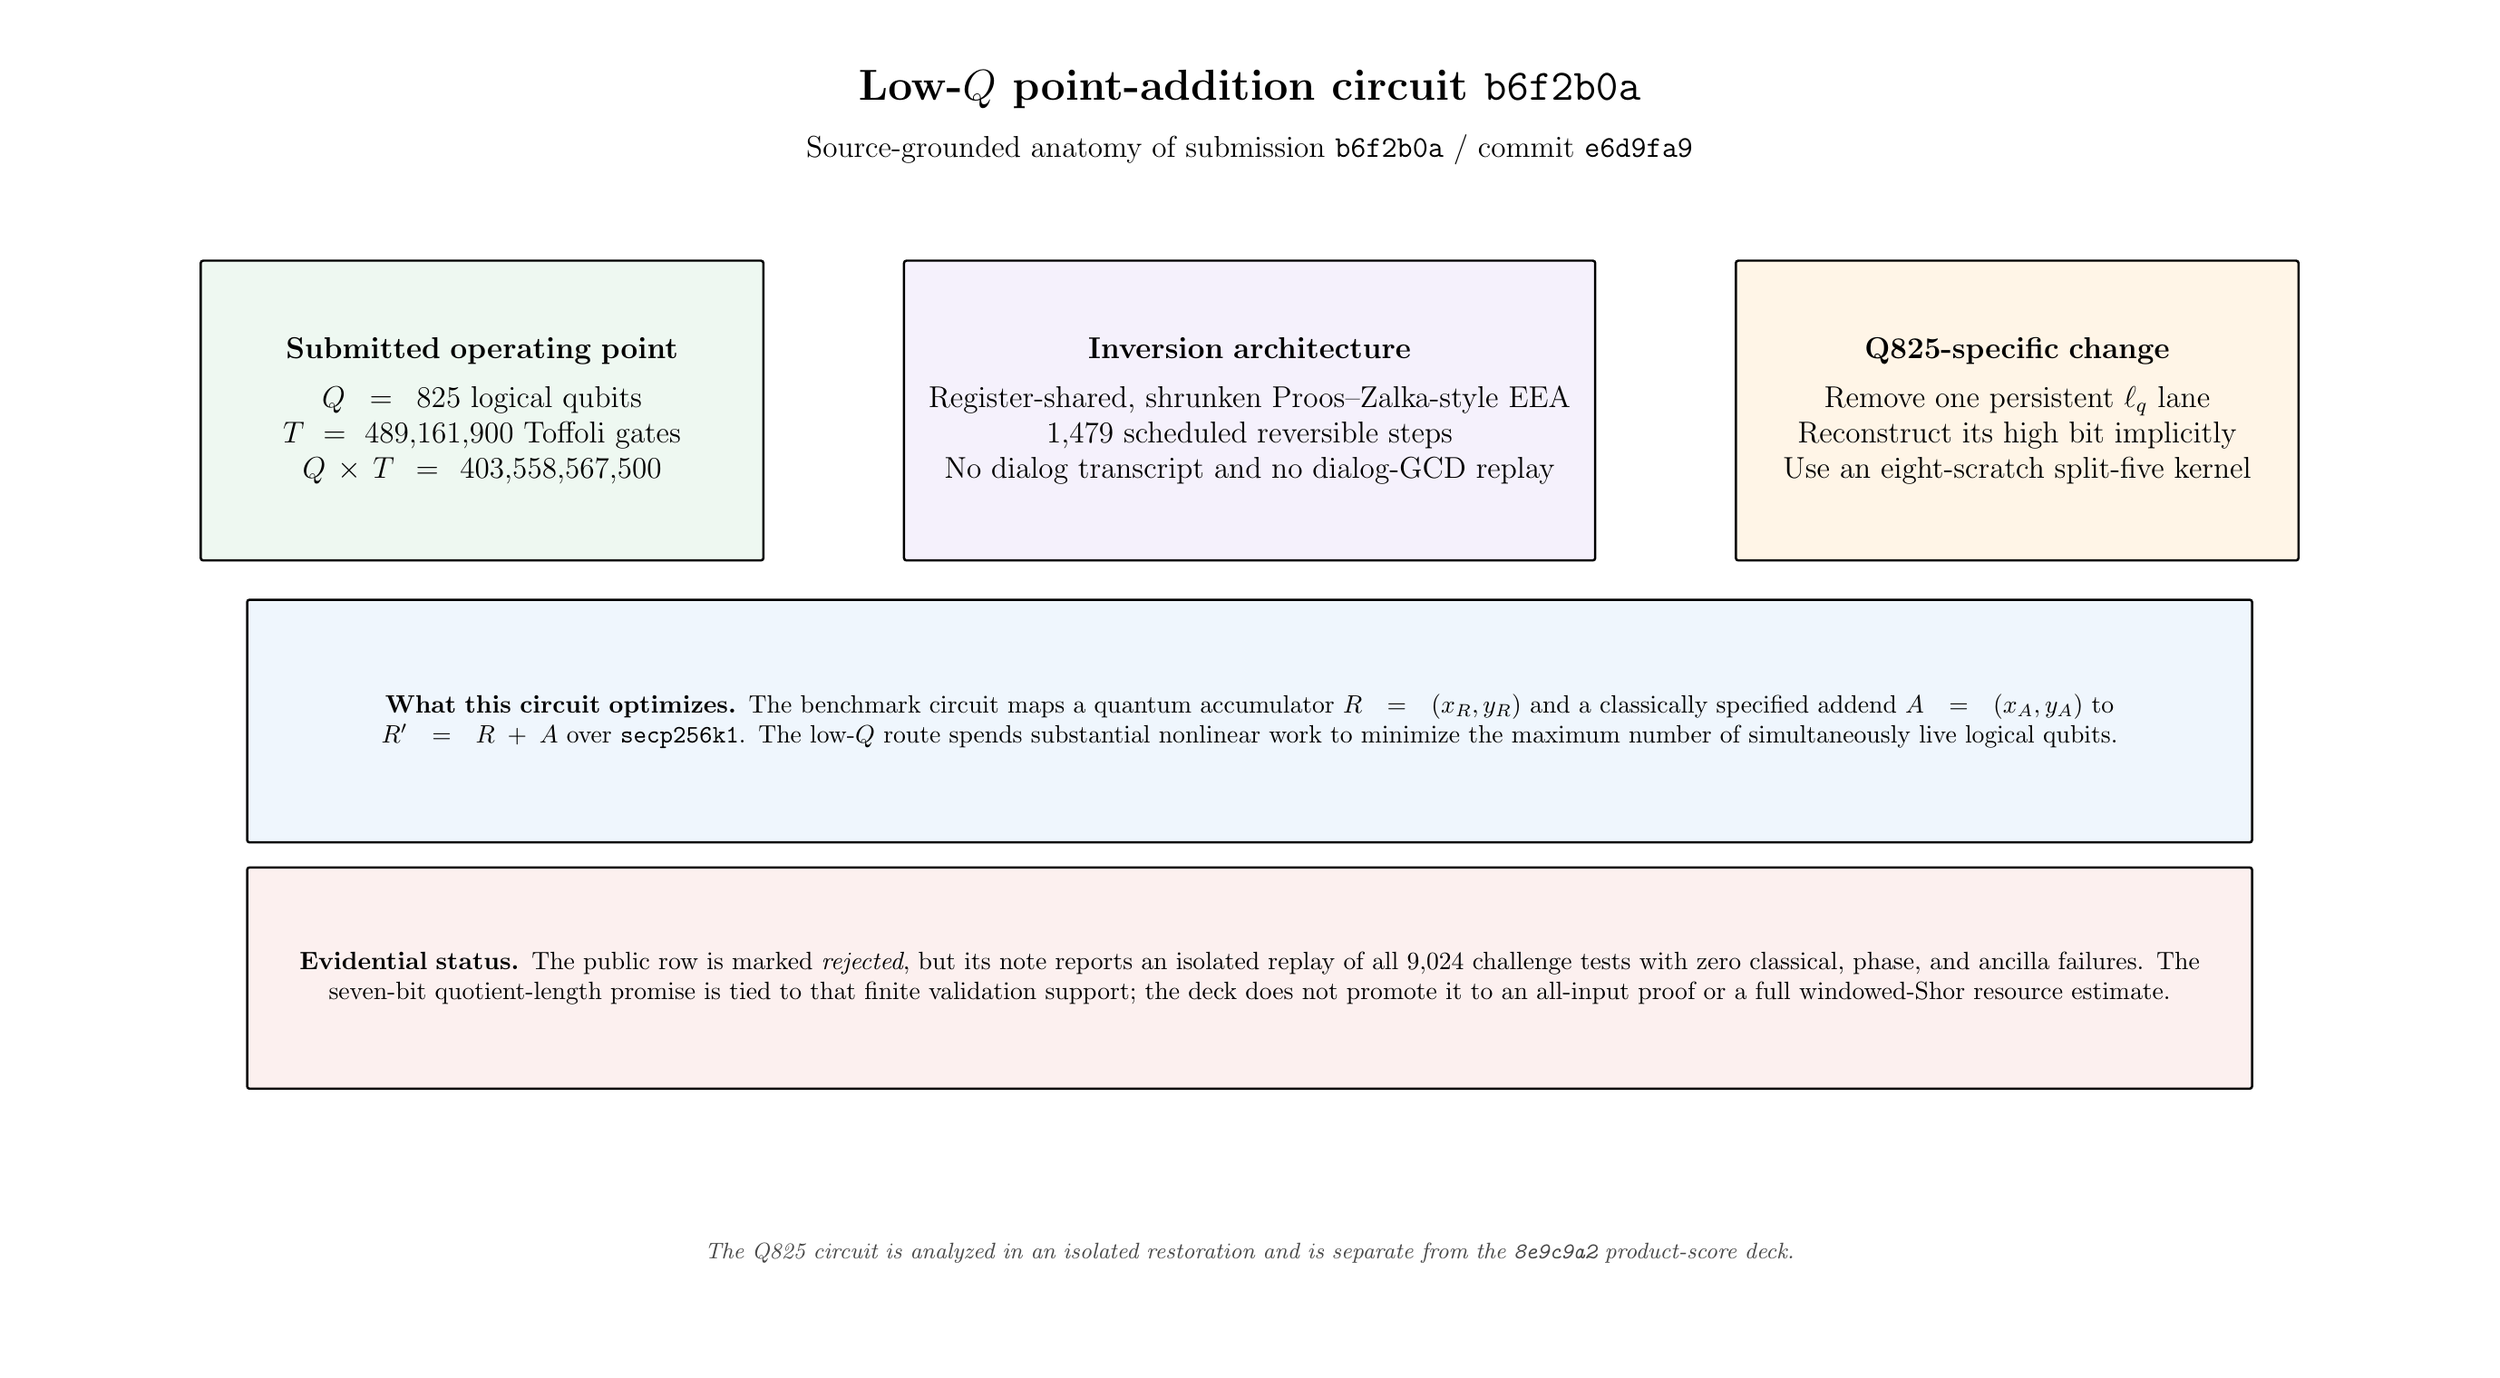
\begin{tikzpicture}[x=1cm,y=1cm]
  \path[use as bounding box] (0,0) rectangle (34.3,18.6);
  \node[font=\LARGE\bfseries] at (17.15,17.7)
    {Low-$Q$ point-addition circuit \texttt{b6f2b0a}};
  \node[font=\large] at (17.15,16.85)
    {Source-grounded anatomy of submission \texttt{b6f2b0a} / commit \texttt{e6d9fa9}};

  \node[result,text width=76mm,minimum height=42mm,font=\large] at (6.4,13.2)
    {\textbf{Submitted operating point}\\[2mm]
     $Q=825$ logical qubits\\
     $T=489{,}161{,}900$ Toffoli gates\\
     $Q\times T=403{,}558{,}567{,}500$};
  \node[inversion,text width=94mm,minimum height=42mm,font=\large] at (17.15,13.2)
    {\textbf{Inversion architecture}\\[2mm]
     Register-shared, shrunken Proos--Zalka-style EEA\\
     $1{,}479$ scheduled reversible steps\\
     No dialog transcript and no dialog-GCD replay};
  \node[classical,text width=76mm,minimum height=42mm,font=\large] at (27.9,13.2)
    {\textbf{Q825-specific change}\\[2mm]
     Remove one persistent $\ell_q$ lane\\
     Reconstruct its high bit implicitly\\
     Use an eight-scratch split-five kernel};

  \node[detailwide,text width=278mm,minimum height=34mm] at (17.15,8.85)
    {\textbf{What this circuit optimizes.} The benchmark circuit maps a quantum accumulator
     $R=(x_R,y_R)$ and a classically specified addend $A=(x_A,y_A)$ to $R'=R+A$ over
     \texttt{secp256k1}. The low-$Q$ route spends substantial nonlinear work to minimize the
     maximum number of simultaneously live logical qubits.};

  \node[warning,text width=278mm,minimum height=31mm] at (17.15,5.25)
    {\textbf{Evidential status.} The public row is marked \emph{rejected}, but its note reports an
     isolated replay of all $9{,}024$ challenge tests with zero classical, phase, and ancilla
     failures. The seven-bit quotient-length promise is tied to that finite validation support;
     the deck does not promote it to an all-input proof or a full windowed-Shor resource estimate.};

  \node[note,text width=29cm,align=center,font=\small\itshape] at (17.15,1.4)
    {The Q825 circuit is analyzed in an isolated restoration and is separate from the
     \texttt{8e9c9a2} product-score deck.};
\end{tikzpicture}
\newpage

% ============================================================================
% Page 2
% ============================================================================
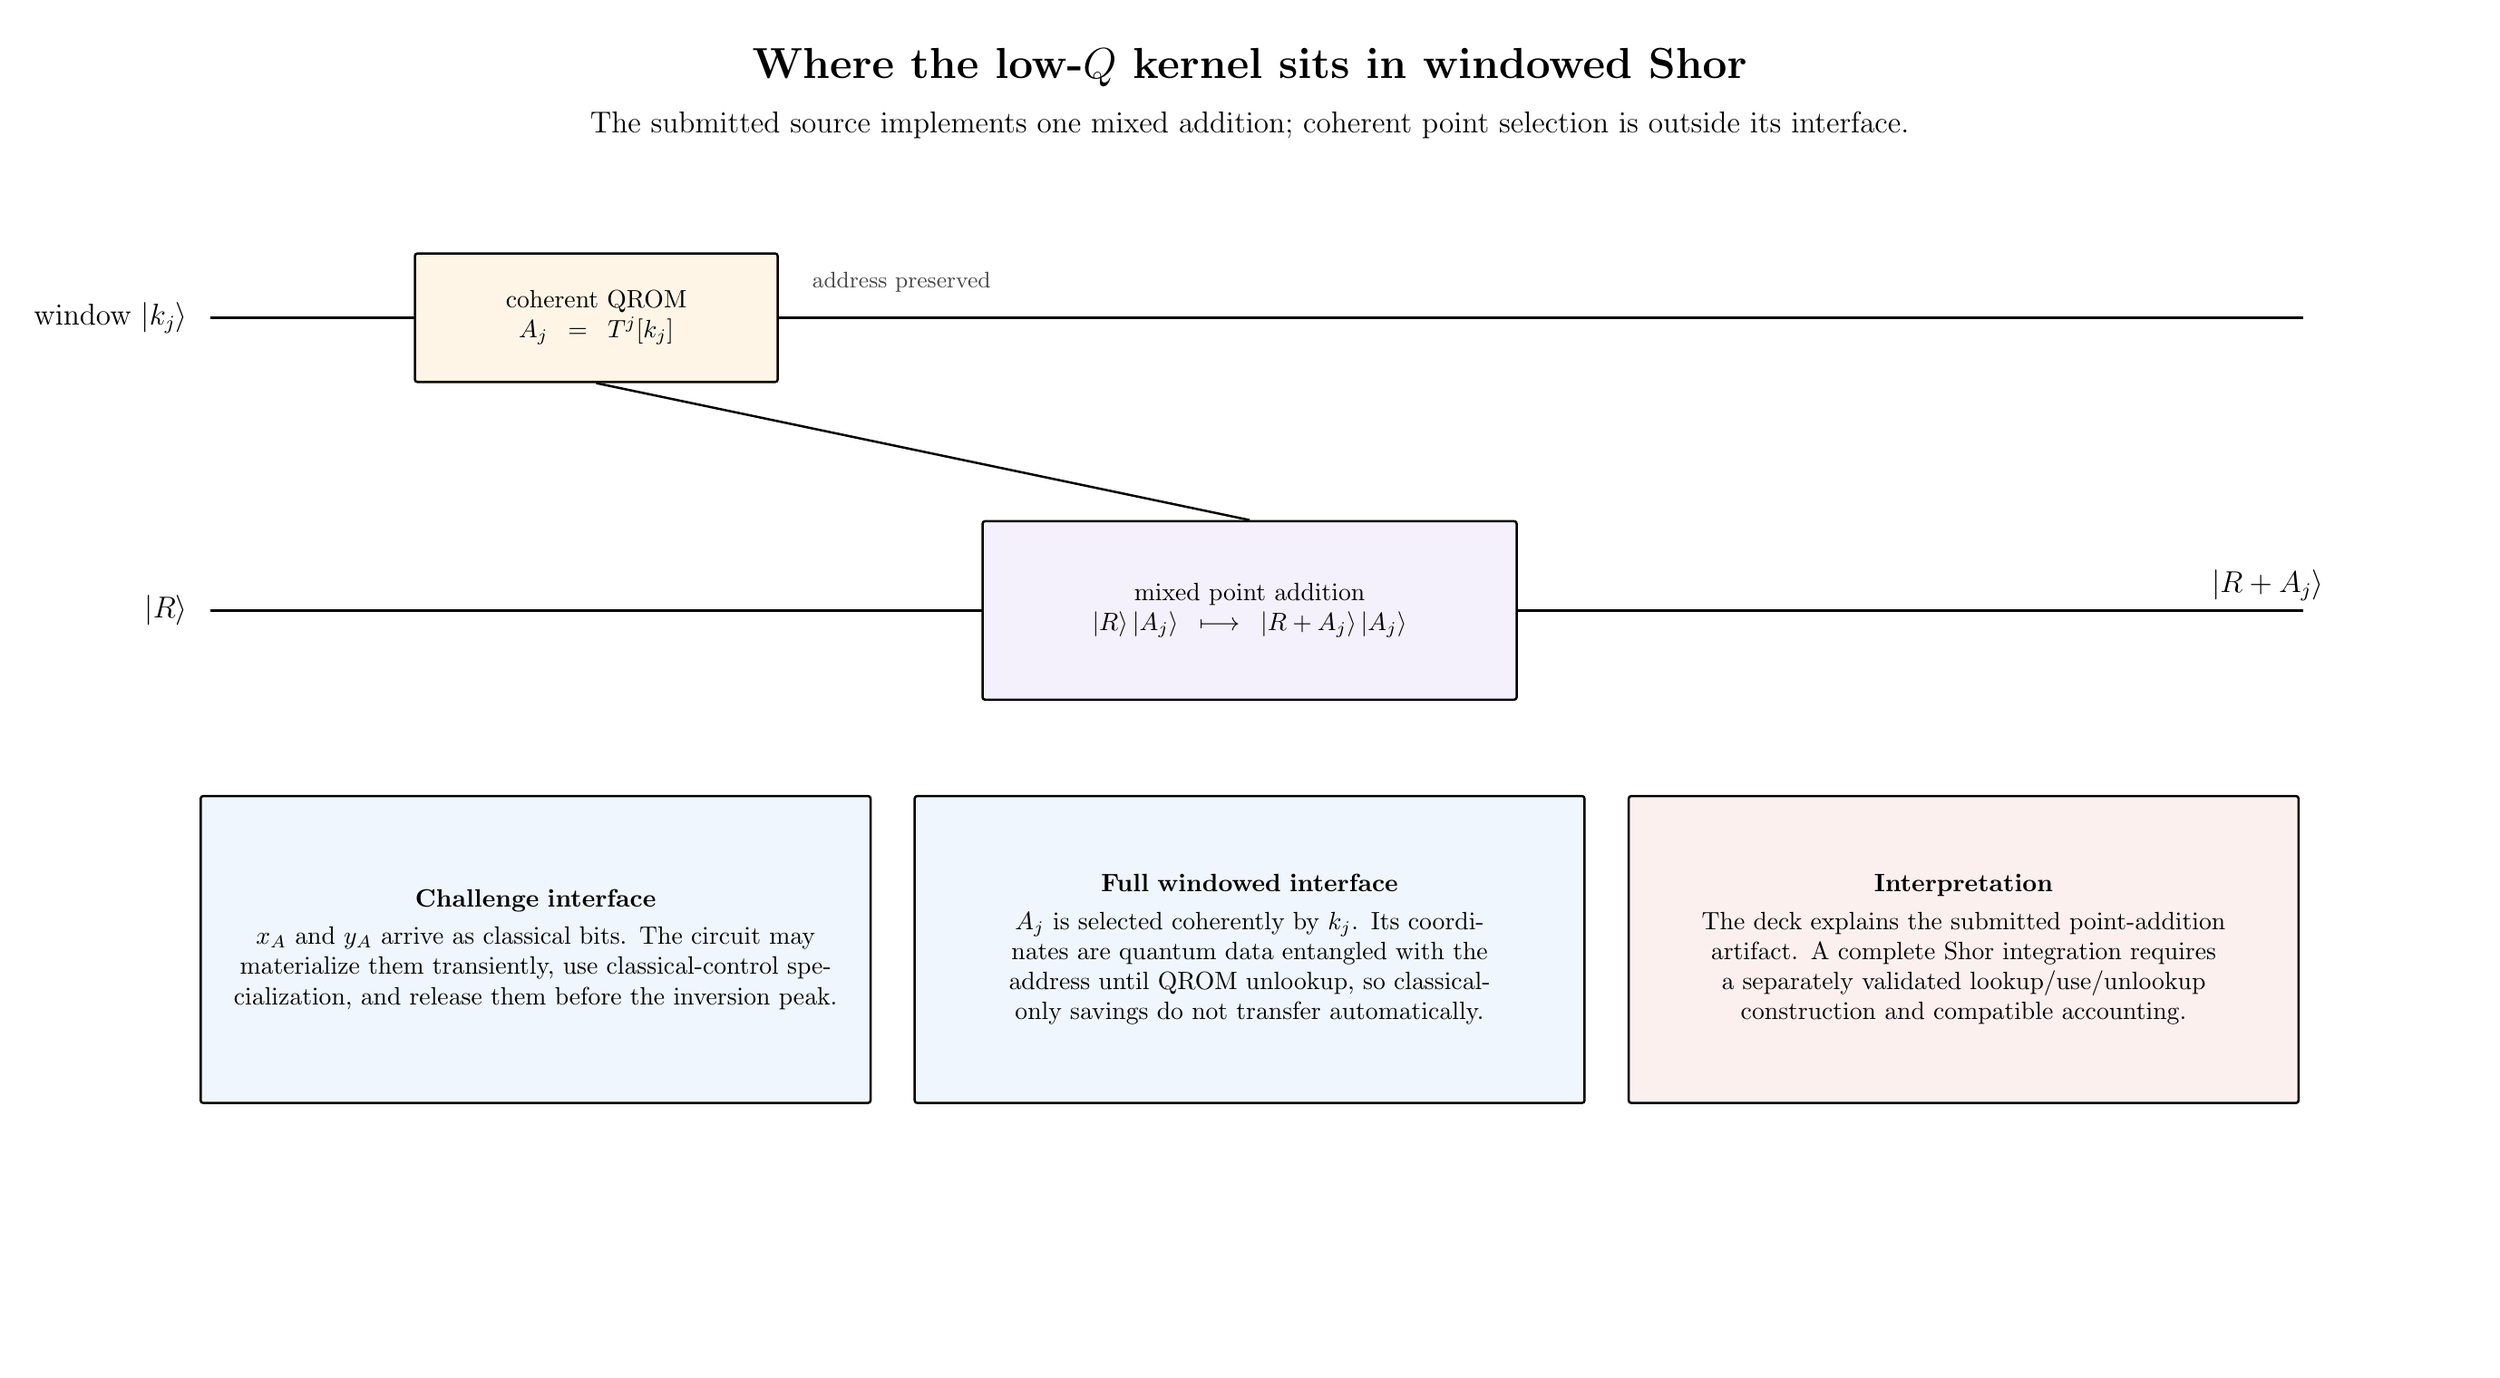
\begin{tikzpicture}[x=1cm,y=1cm]
  \path[use as bounding box] (0,0) rectangle (34.3,18.6);
  \node[font=\LARGE\bfseries] at (17.15,18.0)
    {Where the low-$Q$ kernel sits in windowed Shor};
  \node[font=\large] at (17.15,17.2)
    {The submitted source implements one mixed addition; coherent point selection is outside its interface.};

  \node[lab,anchor=east] at (2.4,14.5) {window $\ket{k_j}$};
  \draw[wire] (2.6,14.5) -- (31.9,14.5);
  \node[classical,text width=48mm,minimum height=18mm] (QROM) at (8.0,14.5)
    {coherent QROM\\$A_j=T^j[k_j]$};
  \node[note,anchor=west] at (10.9,15.0) {address preserved};

  \node[lab,anchor=east] at (2.4,10.4) {$\ket{R}$};
  \draw[wire] (2.6,10.4) -- (31.9,10.4);
  \node[inversion,text width=72mm,minimum height=25mm] (ADD) at (17.15,10.4)
    {mixed point addition\\$\ket{R}\ket{A_j}\longmapsto\ket{R+A_j}\ket{A_j}$};
  \draw[wire] (QROM.south) -- (ADD.north);
  \node[lab,anchor=west] at (30.5,10.75) {$\ket{R+A_j}$};

  \node[detail,text width=91mm,minimum height=43mm] at (7.15,5.65)
    {\textbf{Challenge interface}\\[1mm]
     $x_A$ and $y_A$ arrive as classical bits. The circuit may materialize them transiently,
     use classical-control specialization, and release them before the inversion peak.};
  \node[detail,text width=91mm,minimum height=43mm] at (17.15,5.65)
    {\textbf{Full windowed interface}\\[1mm]
     $A_j$ is selected coherently by $k_j$. Its coordinates are quantum data entangled with
     the address until QROM unlookup, so classical-only savings do not transfer automatically.};
  \node[warning,text width=91mm,minimum height=43mm] at (27.15,5.65)
    {\textbf{Interpretation}\\[1mm]
     The deck explains the submitted point-addition artifact. A complete Shor integration
     requires a separately validated lookup/use/unlookup construction and compatible accounting.};
\end{tikzpicture}
\newpage

% ============================================================================
% Page 3
% ============================================================================
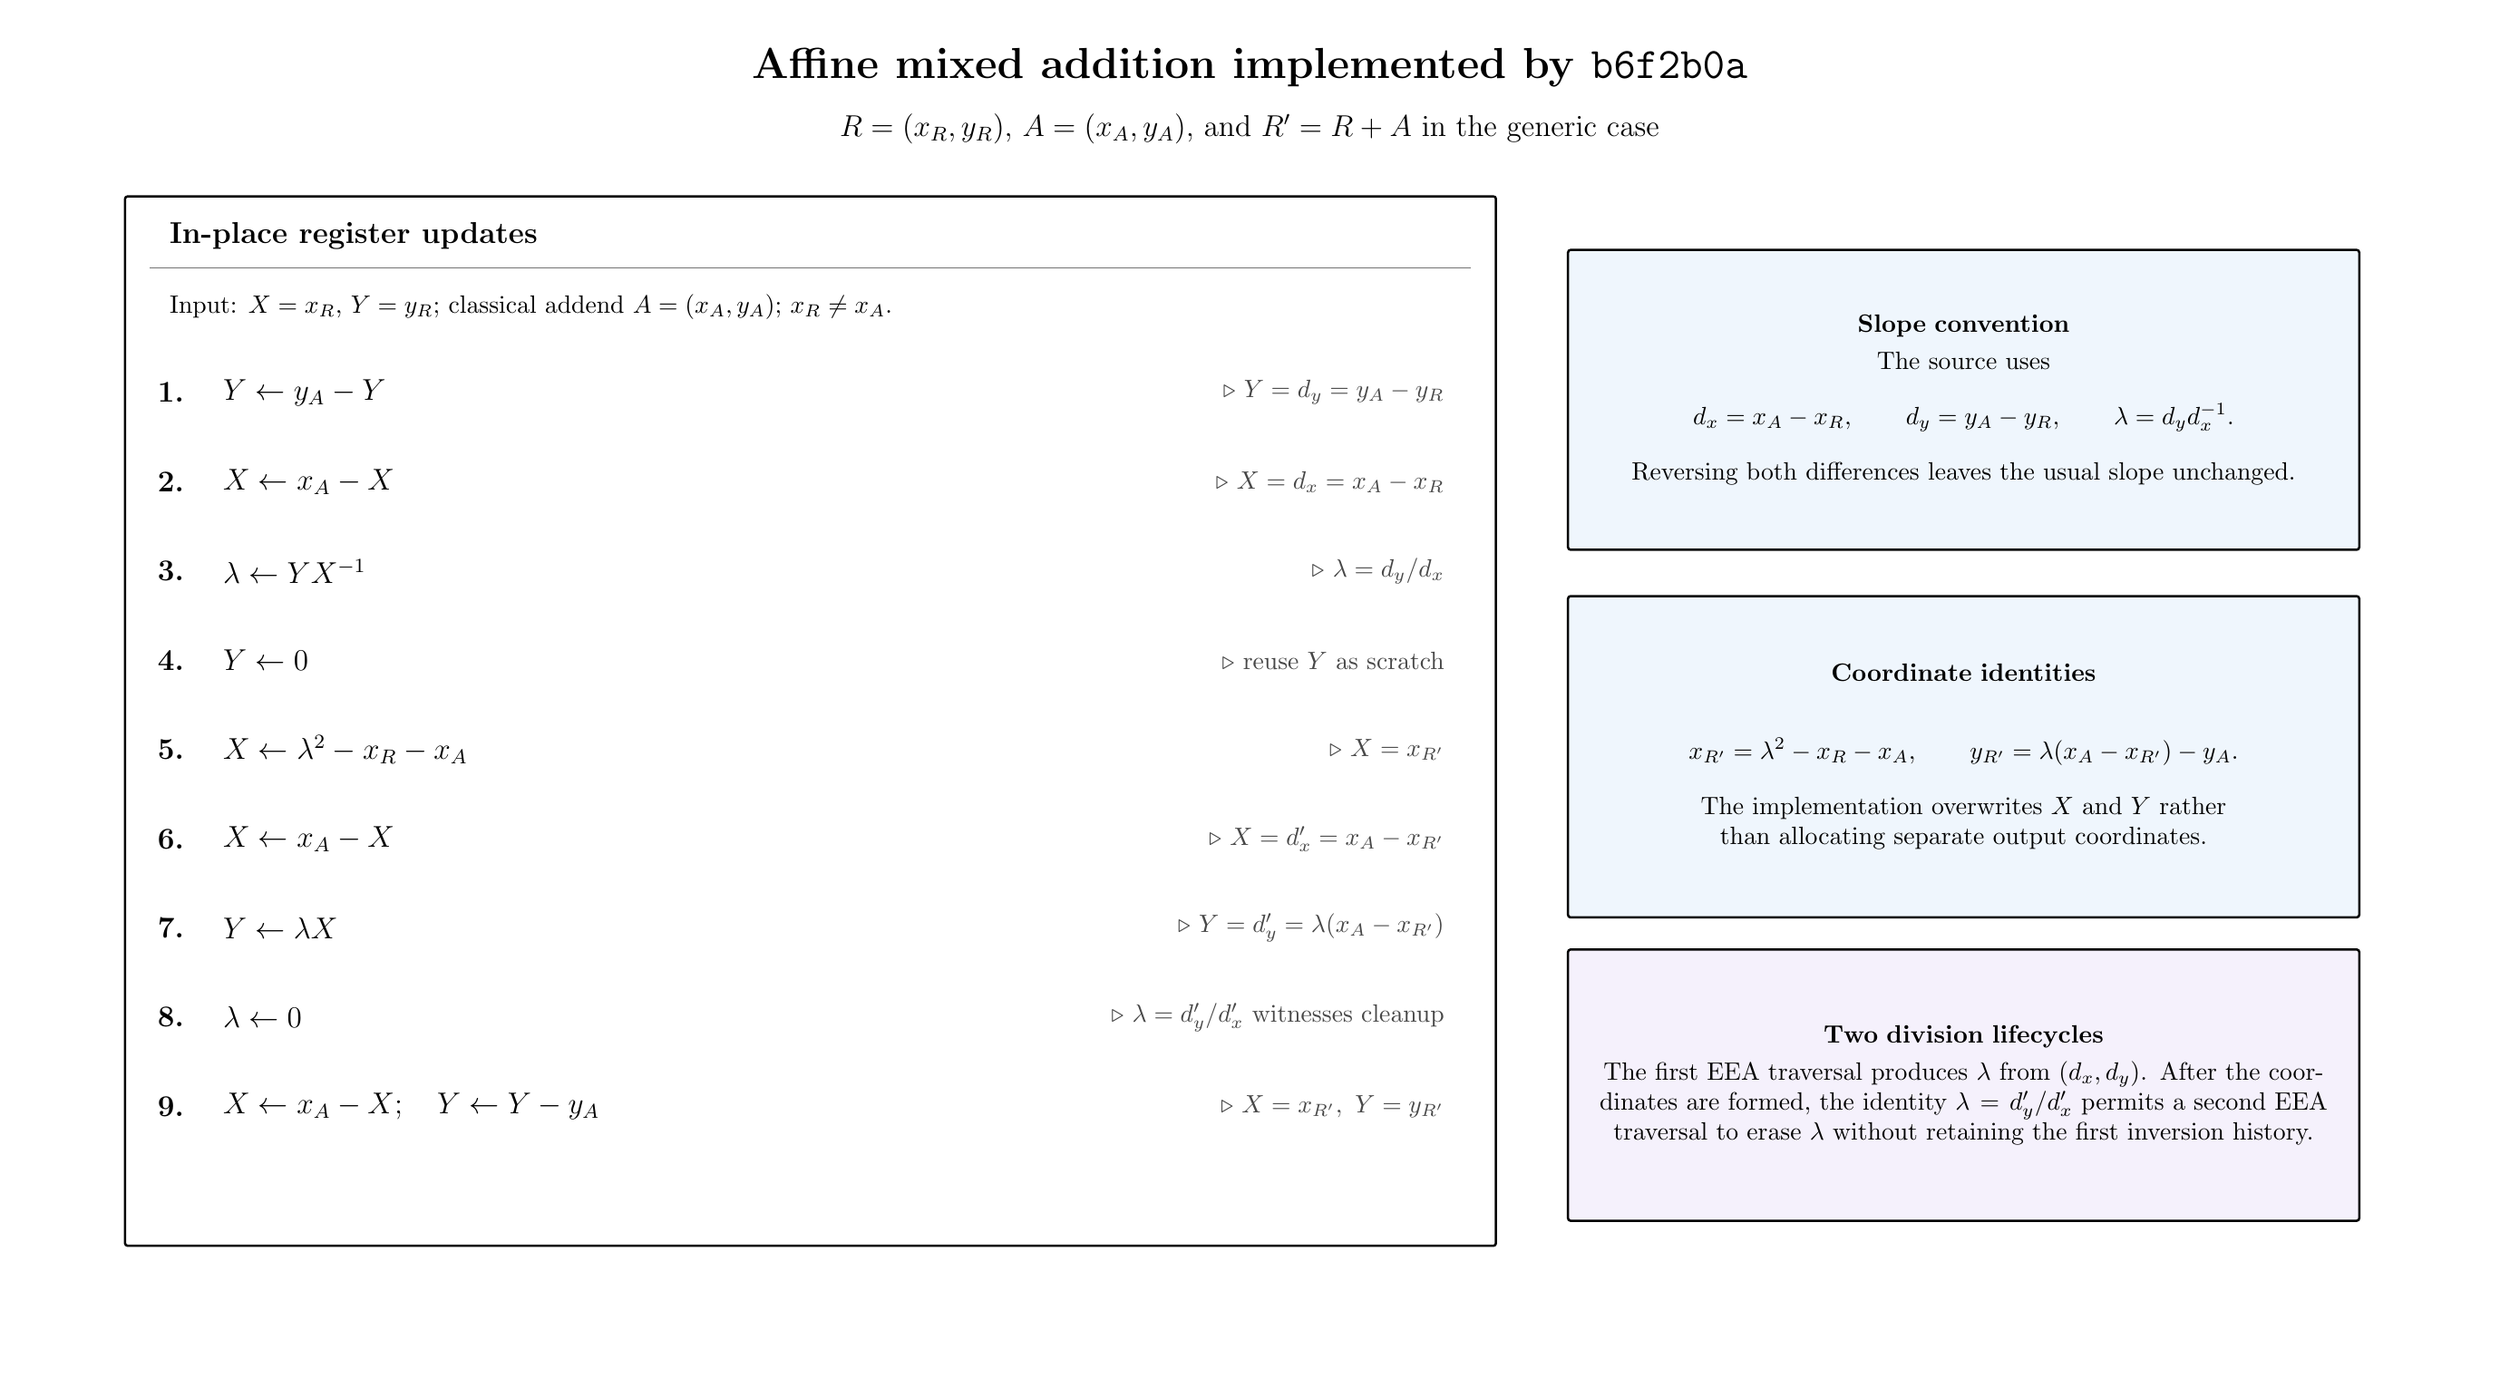
\begin{tikzpicture}[x=1cm,y=1cm]
  \path[use as bounding box] (0,0) rectangle (34.3,18.6);
  \node[font=\LARGE\bfseries] at (17.15,18.0)
    {Affine mixed addition implemented by \texttt{b6f2b0a}};
  \node[font=\large] at (17.15,17.15)
    {$R=(x_R,y_R)$, $A=(x_A,y_A)$, and $R'=R+A$ in the generic case};

  \draw[black,line width=0.9pt,rounded corners=1pt] (1.4,1.5) rectangle (20.6,16.2);
  \node[font=\large\bfseries,anchor=west] at (1.9,15.65) {In-place register updates};
  \draw[black!55] (1.75,15.2) -- (20.25,15.2);
  \node[font=\normalsize,anchor=west] at (1.9,14.65)
    {Input: $X=x_R$, $Y=y_R$; classical addend $A=(x_A,y_A)$; $x_R\ne x_A$.};

  \foreach \n/\yy/\op/\rhs in {
    1/13.45/{Y\gets y_A-Y}/{Y=d_y=y_A-y_R},
    2/12.20/{X\gets x_A-X}/{X=d_x=x_A-x_R},
    3/10.95/{\lambda\gets YX^{-1}}/{\lambda=d_y/d_x},
    4/9.70/{Y\gets 0}/{\text{reuse }Y\text{ as scratch}},
    5/8.45/{X\gets \lambda^2-x_R-x_A}/{X=x_{R'}},
    6/7.20/{X\gets x_A-X}/{X=d'_x=x_A-x_{R'}},
    7/5.95/{Y\gets \lambda X}/{Y=d'_y=\lambda(x_A-x_{R'})},
    8/4.70/{\lambda\gets 0}/{\lambda=d'_y/d'_x\text{ witnesses cleanup}},
    9/3.45/{X\gets x_A-X;\quad Y\gets Y-y_A}/{X=x_{R'},\ Y=y_{R'}}
  }{
    \node[font=\large\bfseries,anchor=east] at (2.35,\yy) {\n.};
    \node[font=\large,anchor=west] at (2.65,\yy) {$\op$};
    \node[font=\normalsize,anchor=east,text=black!72] at (20.0,\yy) {$\triangleright\ \rhs$};
  }

  \node[detail,text width=108mm,minimum height=42mm] at (27.15,13.35)
    {\textbf{Slope convention}\\[1mm]
     The source uses
     \[
       d_x=x_A-x_R,\qquad d_y=y_A-y_R,
       \qquad \lambda=d_y d_x^{-1}.
     \]
     Reversing both differences leaves the usual slope unchanged.};
  \node[detail,text width=108mm,minimum height=45mm] at (27.15,8.35)
    {\textbf{Coordinate identities}\\[-1mm]
     \[
       x_{R'}=\lambda^2-x_R-x_A,
       \qquad y_{R'}=\lambda(x_A-x_{R'})-y_A.
     \]
     The implementation overwrites $X$ and $Y$ rather than allocating separate output coordinates.};
  \node[inversion,text width=108mm,minimum height=38mm] at (27.15,3.75)
    {\textbf{Two division lifecycles}\\[1mm]
     The first EEA traversal produces $\lambda$ from $(d_x,d_y)$. After the coordinates are formed,
     the identity $\lambda=d'_y/d'_x$ permits a second EEA traversal to erase $\lambda$ without retaining the first inversion history.};
\end{tikzpicture}
\newpage

% ============================================================================
% Page 4
% ============================================================================
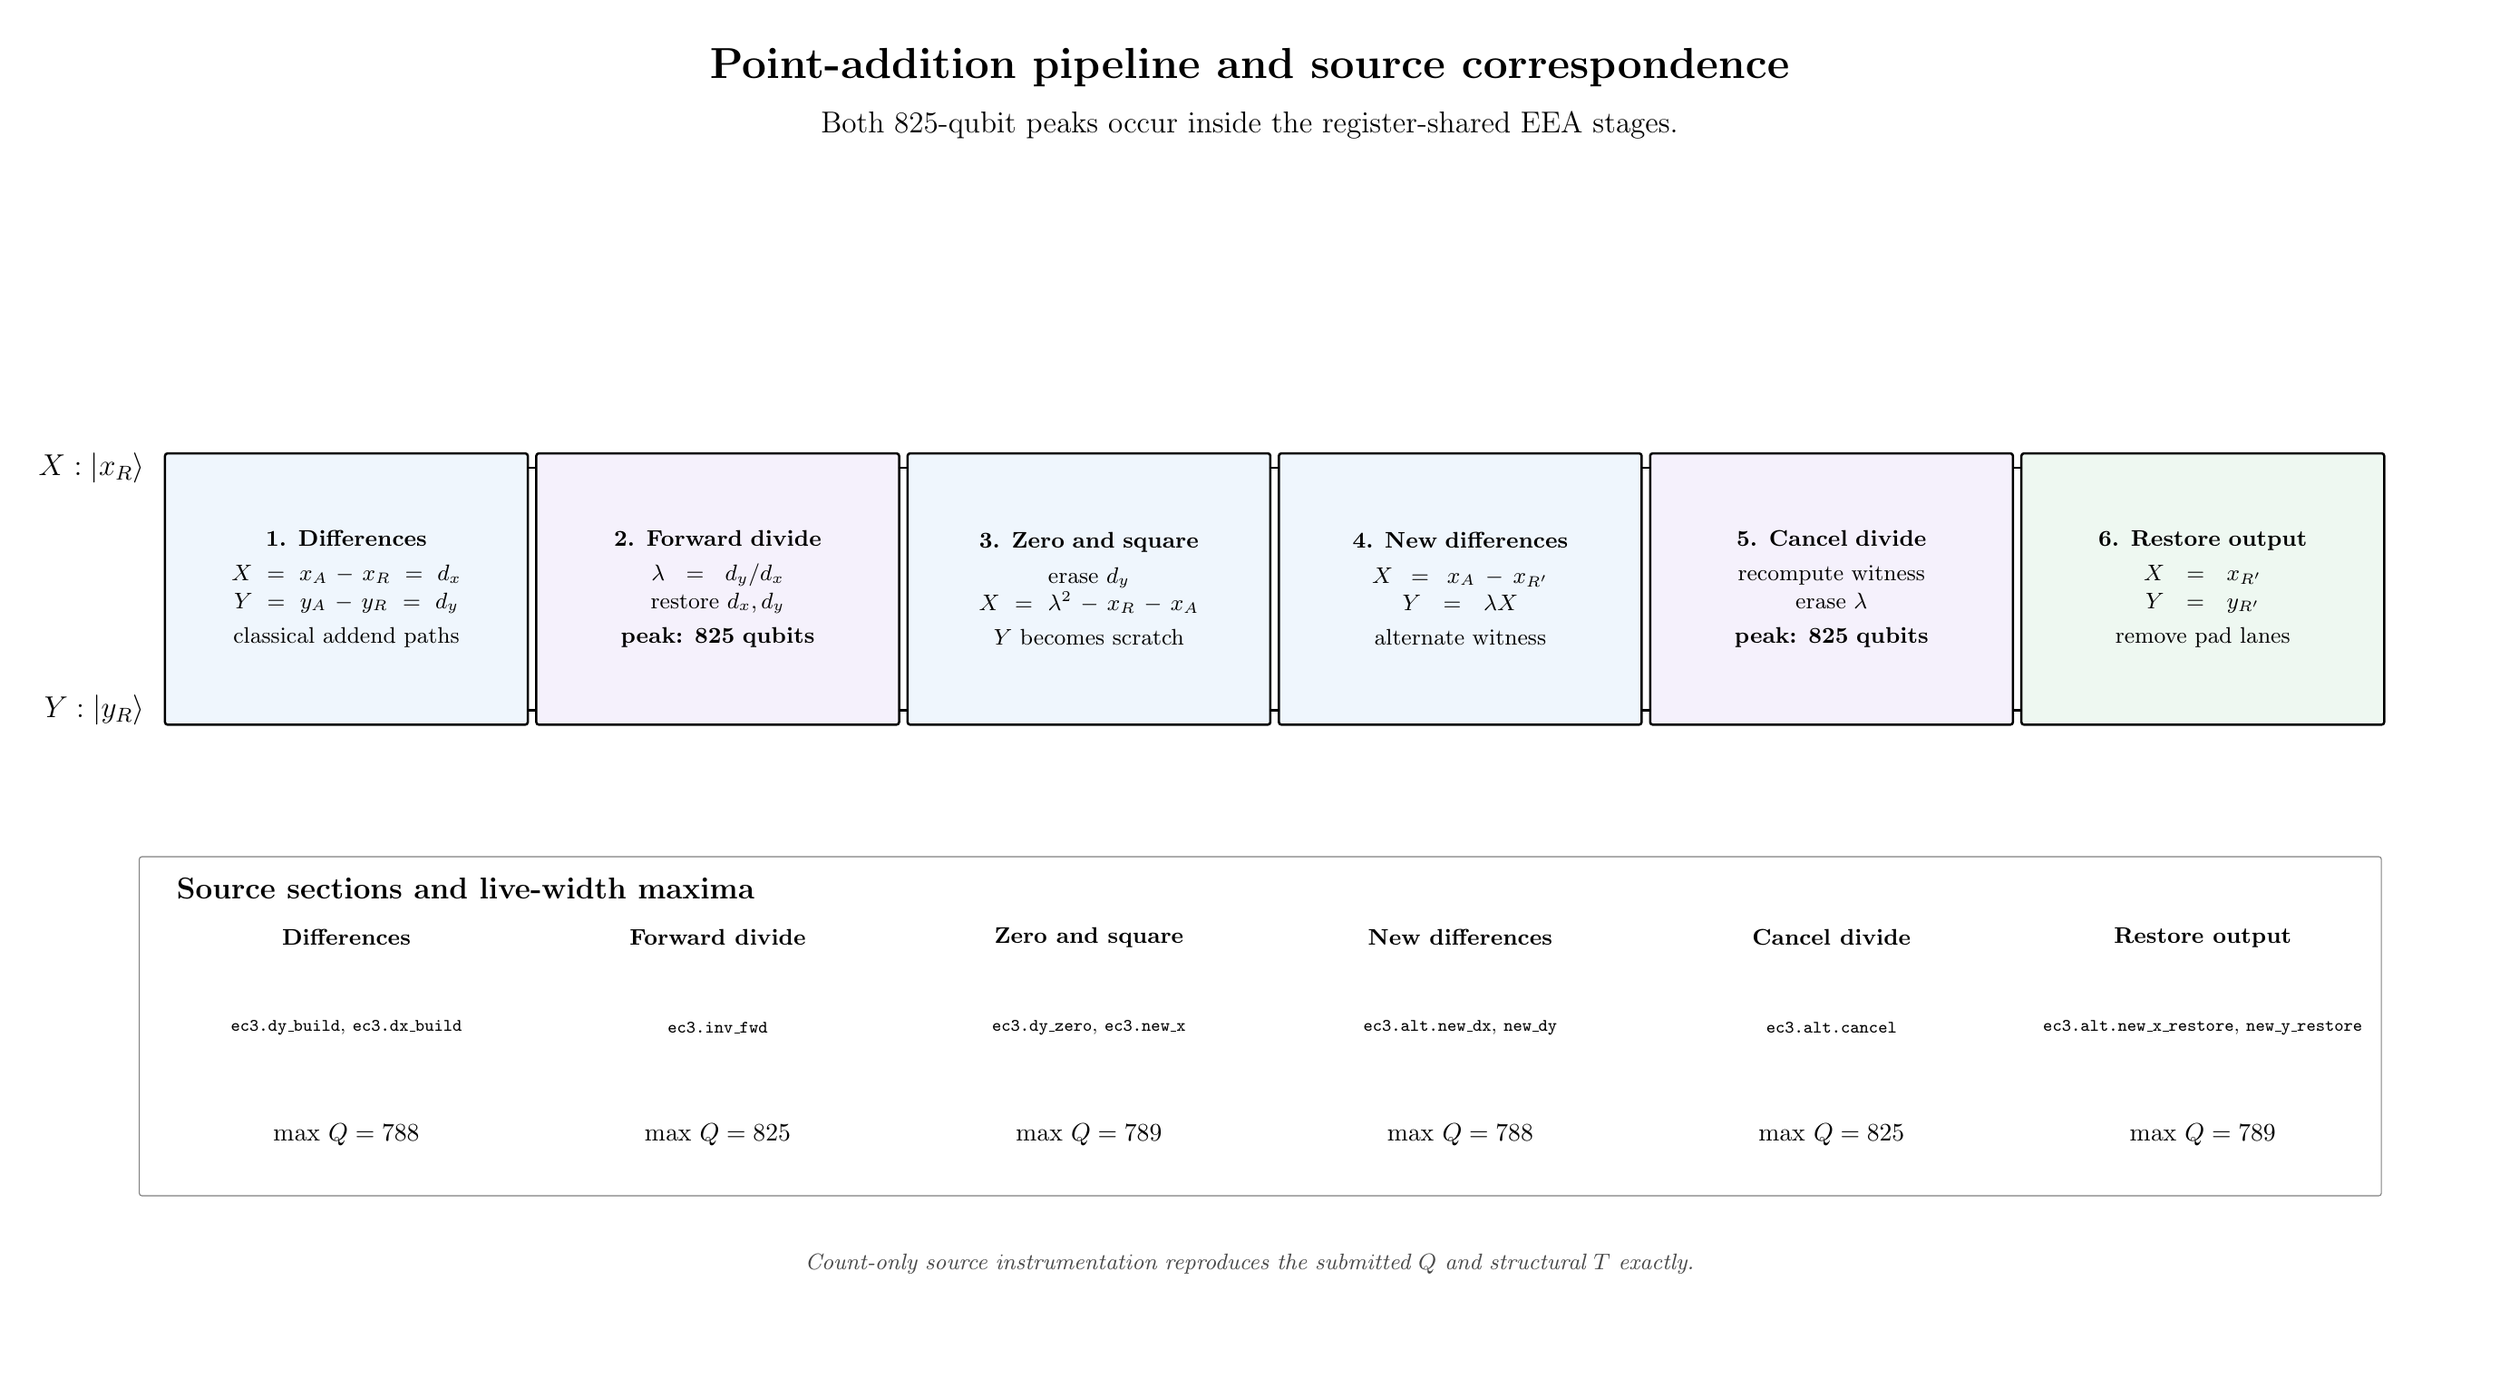
\begin{tikzpicture}[x=1cm,y=1cm]
  \path[use as bounding box] (0,0) rectangle (34.3,18.6);
  \node[font=\LARGE\bfseries] at (17.15,18.0)
    {Point-addition pipeline and source correspondence};
  \node[font=\large] at (17.15,17.2)
    {Both 825-qubit peaks occur inside the register-shared EEA stages.};

  \node[lab,anchor=east] at (1.8,12.4) {$X:\ket{x_R}$};
  \node[lab,anchor=east] at (1.8,9.0) {$Y:\ket{y_R}$};
  \draw[wire] (2.0,12.4) -- (32.8,12.4);
  \draw[wire] (2.0,9.0) -- (32.8,9.0);

  \node[stage] (P1) at (4.5,10.7)
    {\textbf{1. Differences}\\[1mm]
     $X=x_A-x_R=d_x$\\$Y=y_A-y_R=d_y$\\[1mm]
     classical addend paths};
  \node[stage,fill=invviolet] (P2) at (9.7,10.7)
    {\textbf{2. Forward divide}\\[1mm]
     $\lambda=d_y/d_x$\\restore $d_x,d_y$\\[1mm]
     \textbf{peak: 825 qubits}};
  \node[stage] (P3) at (14.9,10.7)
    {\textbf{3. Zero and square}\\[1mm]
     erase $d_y$\\$X=\lambda^2-x_R-x_A$\\[1mm]
     $Y$ becomes scratch};
  \node[stage] (P4) at (20.1,10.7)
    {\textbf{4. New differences}\\[1mm]
     $X=x_A-x_{R'}$\\$Y=\lambda X$\\[1mm]
     alternate witness};
  \node[stage,fill=invviolet] (P5) at (25.3,10.7)
    {\textbf{5. Cancel divide}\\[1mm]
     recompute witness\\erase $\lambda$\\[1mm]
     \textbf{peak: 825 qubits}};
  \node[stage,fill=outgreen] (P6) at (30.5,10.7)
    {\textbf{6. Restore output}\\[1mm]
     $X=x_{R'}$\\$Y=y_{R'}$\\[1mm]
     remove pad lanes};

  \draw[black!50,rounded corners=1pt] (1.6,2.2) rectangle (33.0,6.95);
  \node[font=\large\bfseries,anchor=west] at (2.0,6.5) {Source sections and live-width maxima};
  \foreach \xx/\head/\src/\q in {
    4.5/{Differences}/{\texttt{ec3.dy\_build},\ \texttt{ec3.dx\_build}}/788,
    9.7/{Forward divide}/{\texttt{ec3.inv\_fwd}}/825,
    14.9/{Zero and square}/{\texttt{ec3.dy\_zero},\ \texttt{ec3.new\_x}}/789,
    20.1/{New differences}/{\texttt{ec3.alt.new\_dx},\ \texttt{new\_dy}}/788,
    25.3/{Cancel divide}/{\texttt{ec3.alt.cancel}}/825,
    30.5/{Restore output}/{\texttt{ec3.alt.new\_x\_restore},\ \texttt{new\_y\_restore}}/789
  }{
    \node[font=\small\bfseries] at (\xx,5.82) {\head};
    \node[font=\scriptsize,text width=45mm,align=center] at (\xx,4.55) {\src};
    \node[font=\normalsize] at (\xx,3.05) {max $Q=\q$};
  }
  \node[note,text width=30cm,align=center,font=\small\itshape] at (17.15,1.25)
    {Count-only source instrumentation reproduces the submitted $Q$ and structural $T$ exactly.};
\end{tikzpicture}
\newpage

% ============================================================================
% Additional analysis: exact live-set accounting at the EEA peak
% ============================================================================
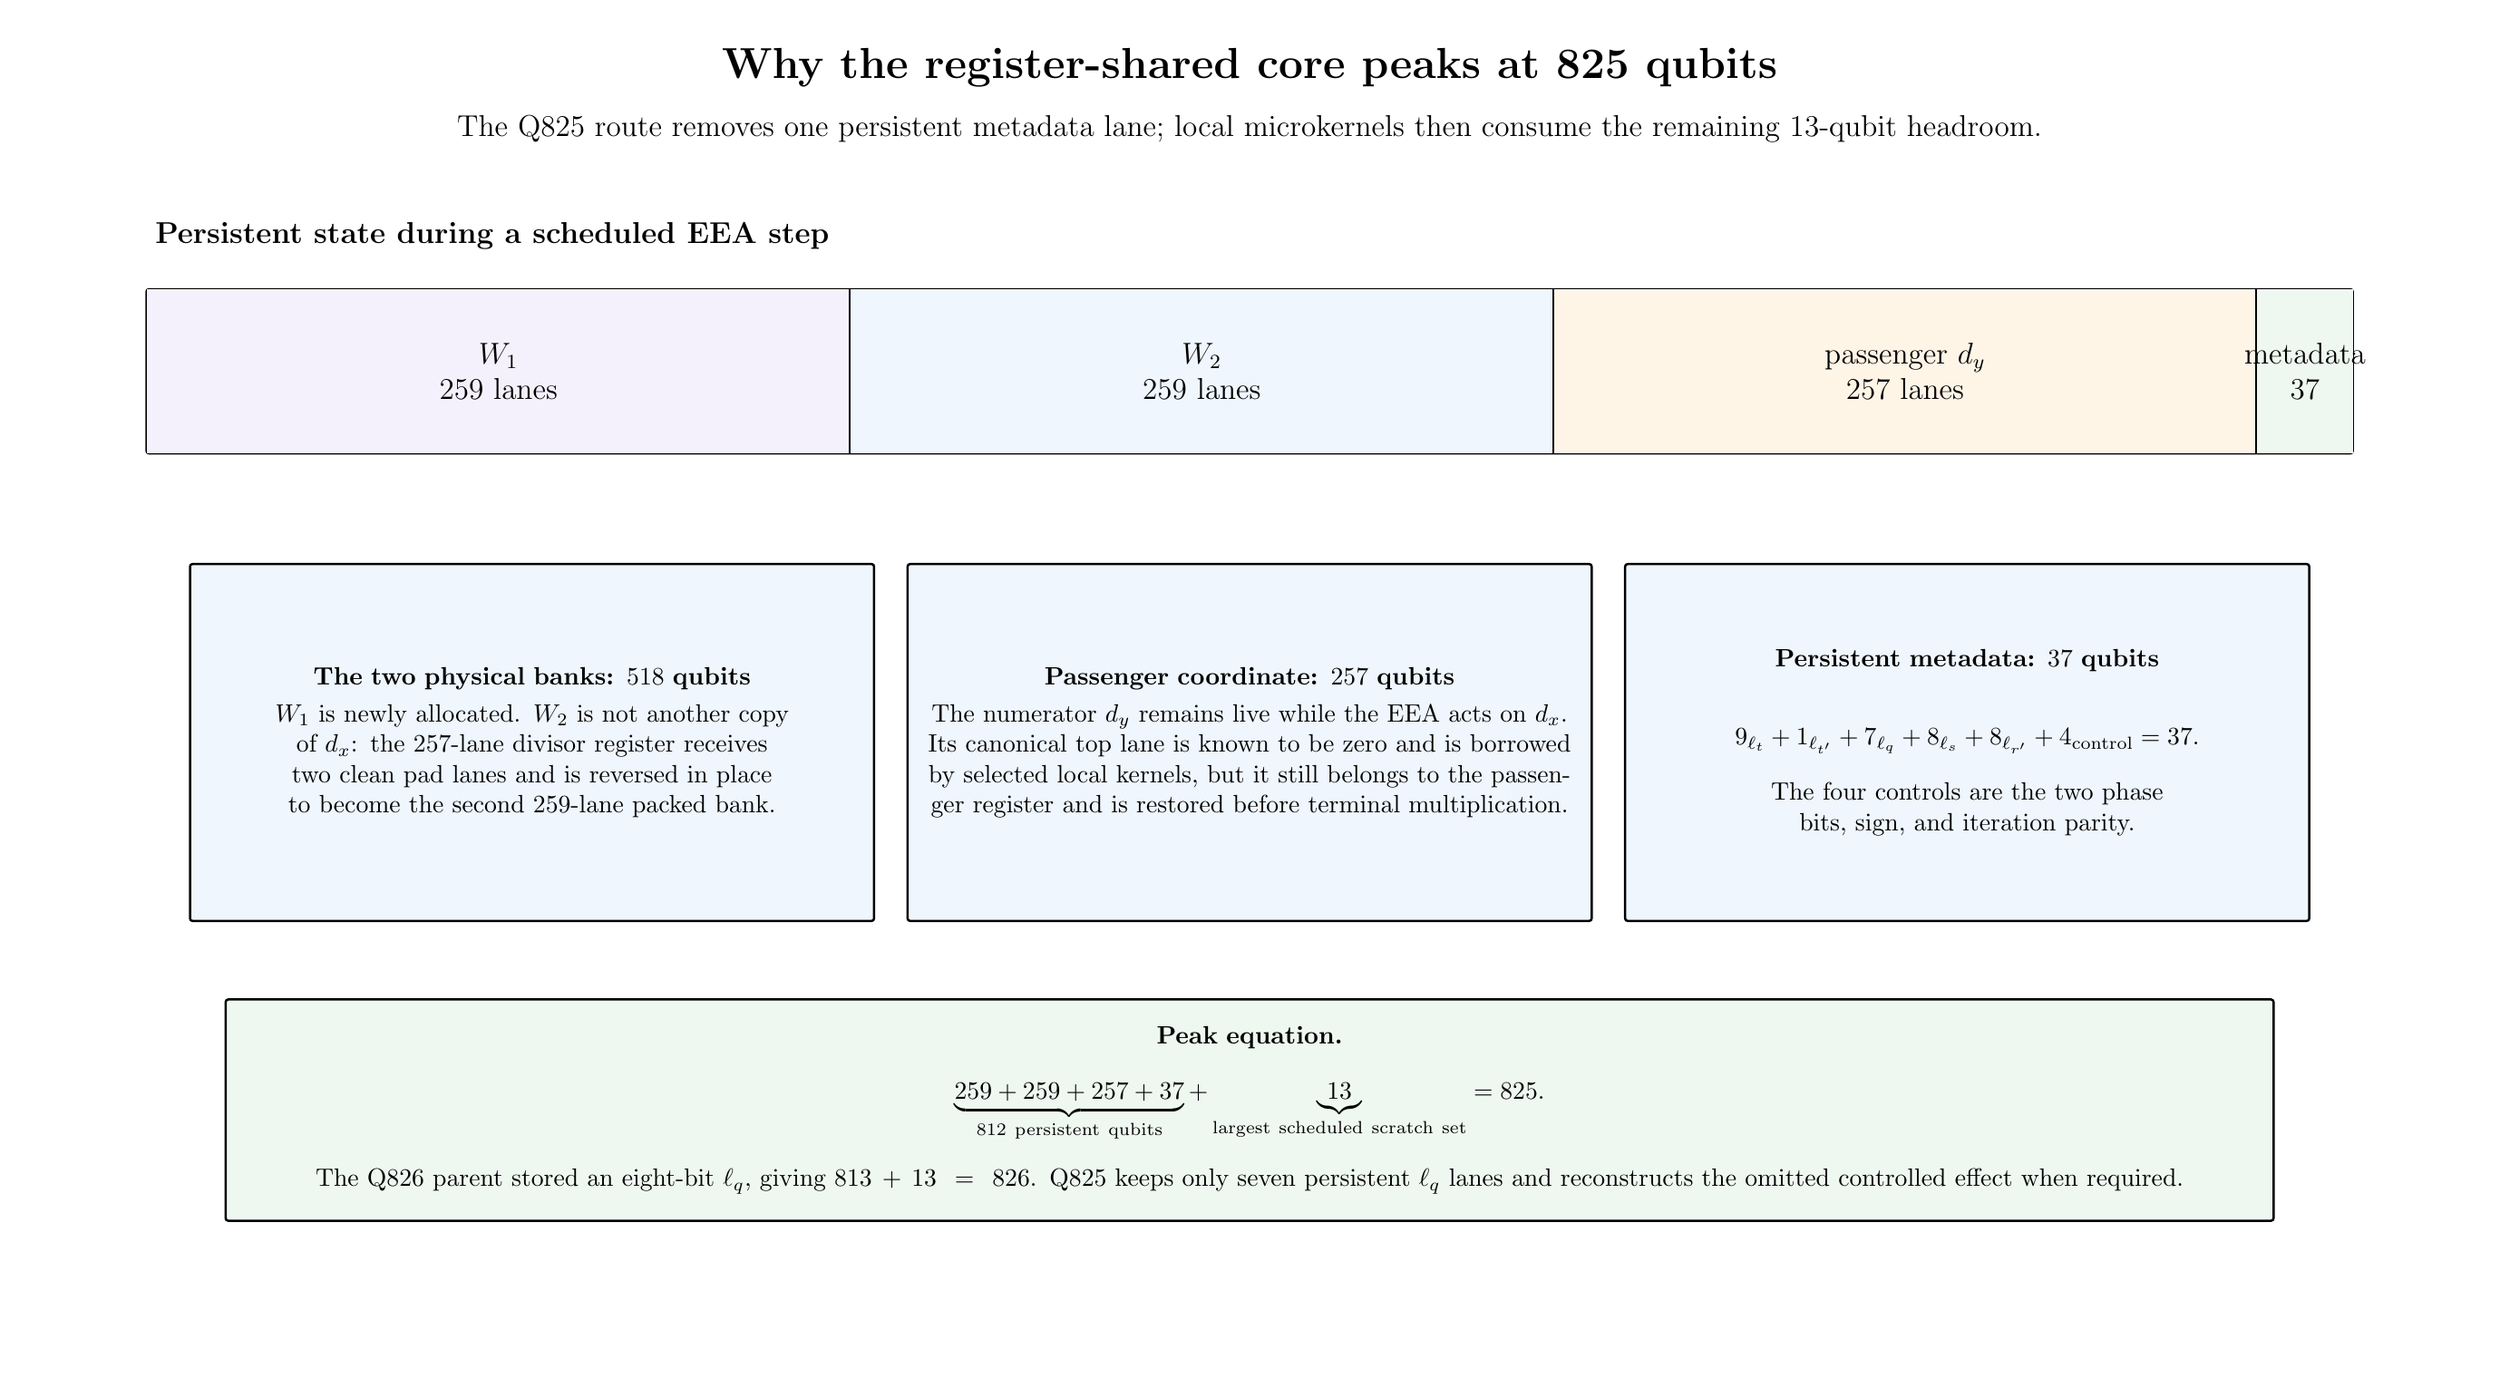
\begin{tikzpicture}[x=1cm,y=1cm]
  \path[use as bounding box] (0,0) rectangle (34.3,18.6);
  \node[font=\LARGE\bfseries] at (17.15,18.0)
    {Why the register-shared core peaks at 825 qubits};
  \node[font=\large] at (17.15,17.15)
    {The Q825 route removes one persistent metadata lane; local microkernels then consume the remaining 13-qubit headroom.};

  \node[font=\large\bfseries,anchor=west] at (1.7,15.65) {Persistent state during a scheduled EEA step};
  \draw[black,line width=0.9pt,rounded corners=1pt] (1.7,12.6) rectangle (32.6,14.9);
  \fill[invviolet] (1.7,12.6) rectangle (11.55,14.9);
  \fill[gateblue] (11.55,12.6) rectangle (21.4,14.9);
  \fill[lookorange] (21.4,12.6) rectangle (31.25,14.9);
  \fill[outgreen] (31.25,12.6) rectangle (32.6,14.9);
  \foreach \xx in {11.55,21.4,31.25}{\draw[black,line width=0.7pt] (\xx,12.6)--(\xx,14.9);}
  \node[font=\large,align=center] at (6.63,13.75) {$W_1$\\$259$ lanes};
  \node[font=\large,align=center] at (16.48,13.75) {$W_2$\\$259$ lanes};
  \node[font=\large,align=center] at (26.33,13.75) {passenger $d_y$\\$257$ lanes};
  \node[font=\large,align=center] at (31.93,13.75) {metadata\\$37$};

  \node[detail,text width=93mm,minimum height=50mm] at (7.1,8.55)
    {\textbf{The two physical banks: $518$ qubits}\\[1mm]
     $W_1$ is newly allocated. $W_2$ is not another copy of $d_x$: the $257$-lane
     divisor register receives two clean pad lanes and is reversed in place to become
     the second $259$-lane packed bank.};
  \node[detail,text width=93mm,minimum height=50mm] at (17.15,8.55)
    {\textbf{Passenger coordinate: $257$ qubits}\\[1mm]
     The numerator $d_y$ remains live while the EEA acts on $d_x$. Its canonical top
     lane is known to be zero and is borrowed by selected local kernels, but it still
     belongs to the passenger register and is restored before terminal multiplication.};
  \node[detail,text width=93mm,minimum height=50mm] at (27.2,8.55)
    {\textbf{Persistent metadata: $37$ qubits}\\[-1mm]
     \[
       9_{\ell_t}+1_{\ell_{t'}}+7_{\ell_q}+8_{\ell_s}
       +8_{\ell_{r'}}+4_{\rm control}=37.
     \]
     The four controls are the two phase bits, sign, and iteration parity.};

  \node[result,text width=284mm,minimum height=31mm] at (17.15,3.4)
    {\textbf{Peak equation.}
     \[
       \underbrace{259+259+257+37}_{812\ \text{persistent qubits}}
       +\underbrace{13}_{\text{largest scheduled scratch set}}=825.
     \]
     The Q826 parent stored an eight-bit $\ell_q$, giving $813+13=826$. Q825 keeps only seven
     persistent $\ell_q$ lanes and reconstructs the omitted controlled effect when required.};
\end{tikzpicture}
\newpage

% ============================================================================
% Page 5
% ============================================================================
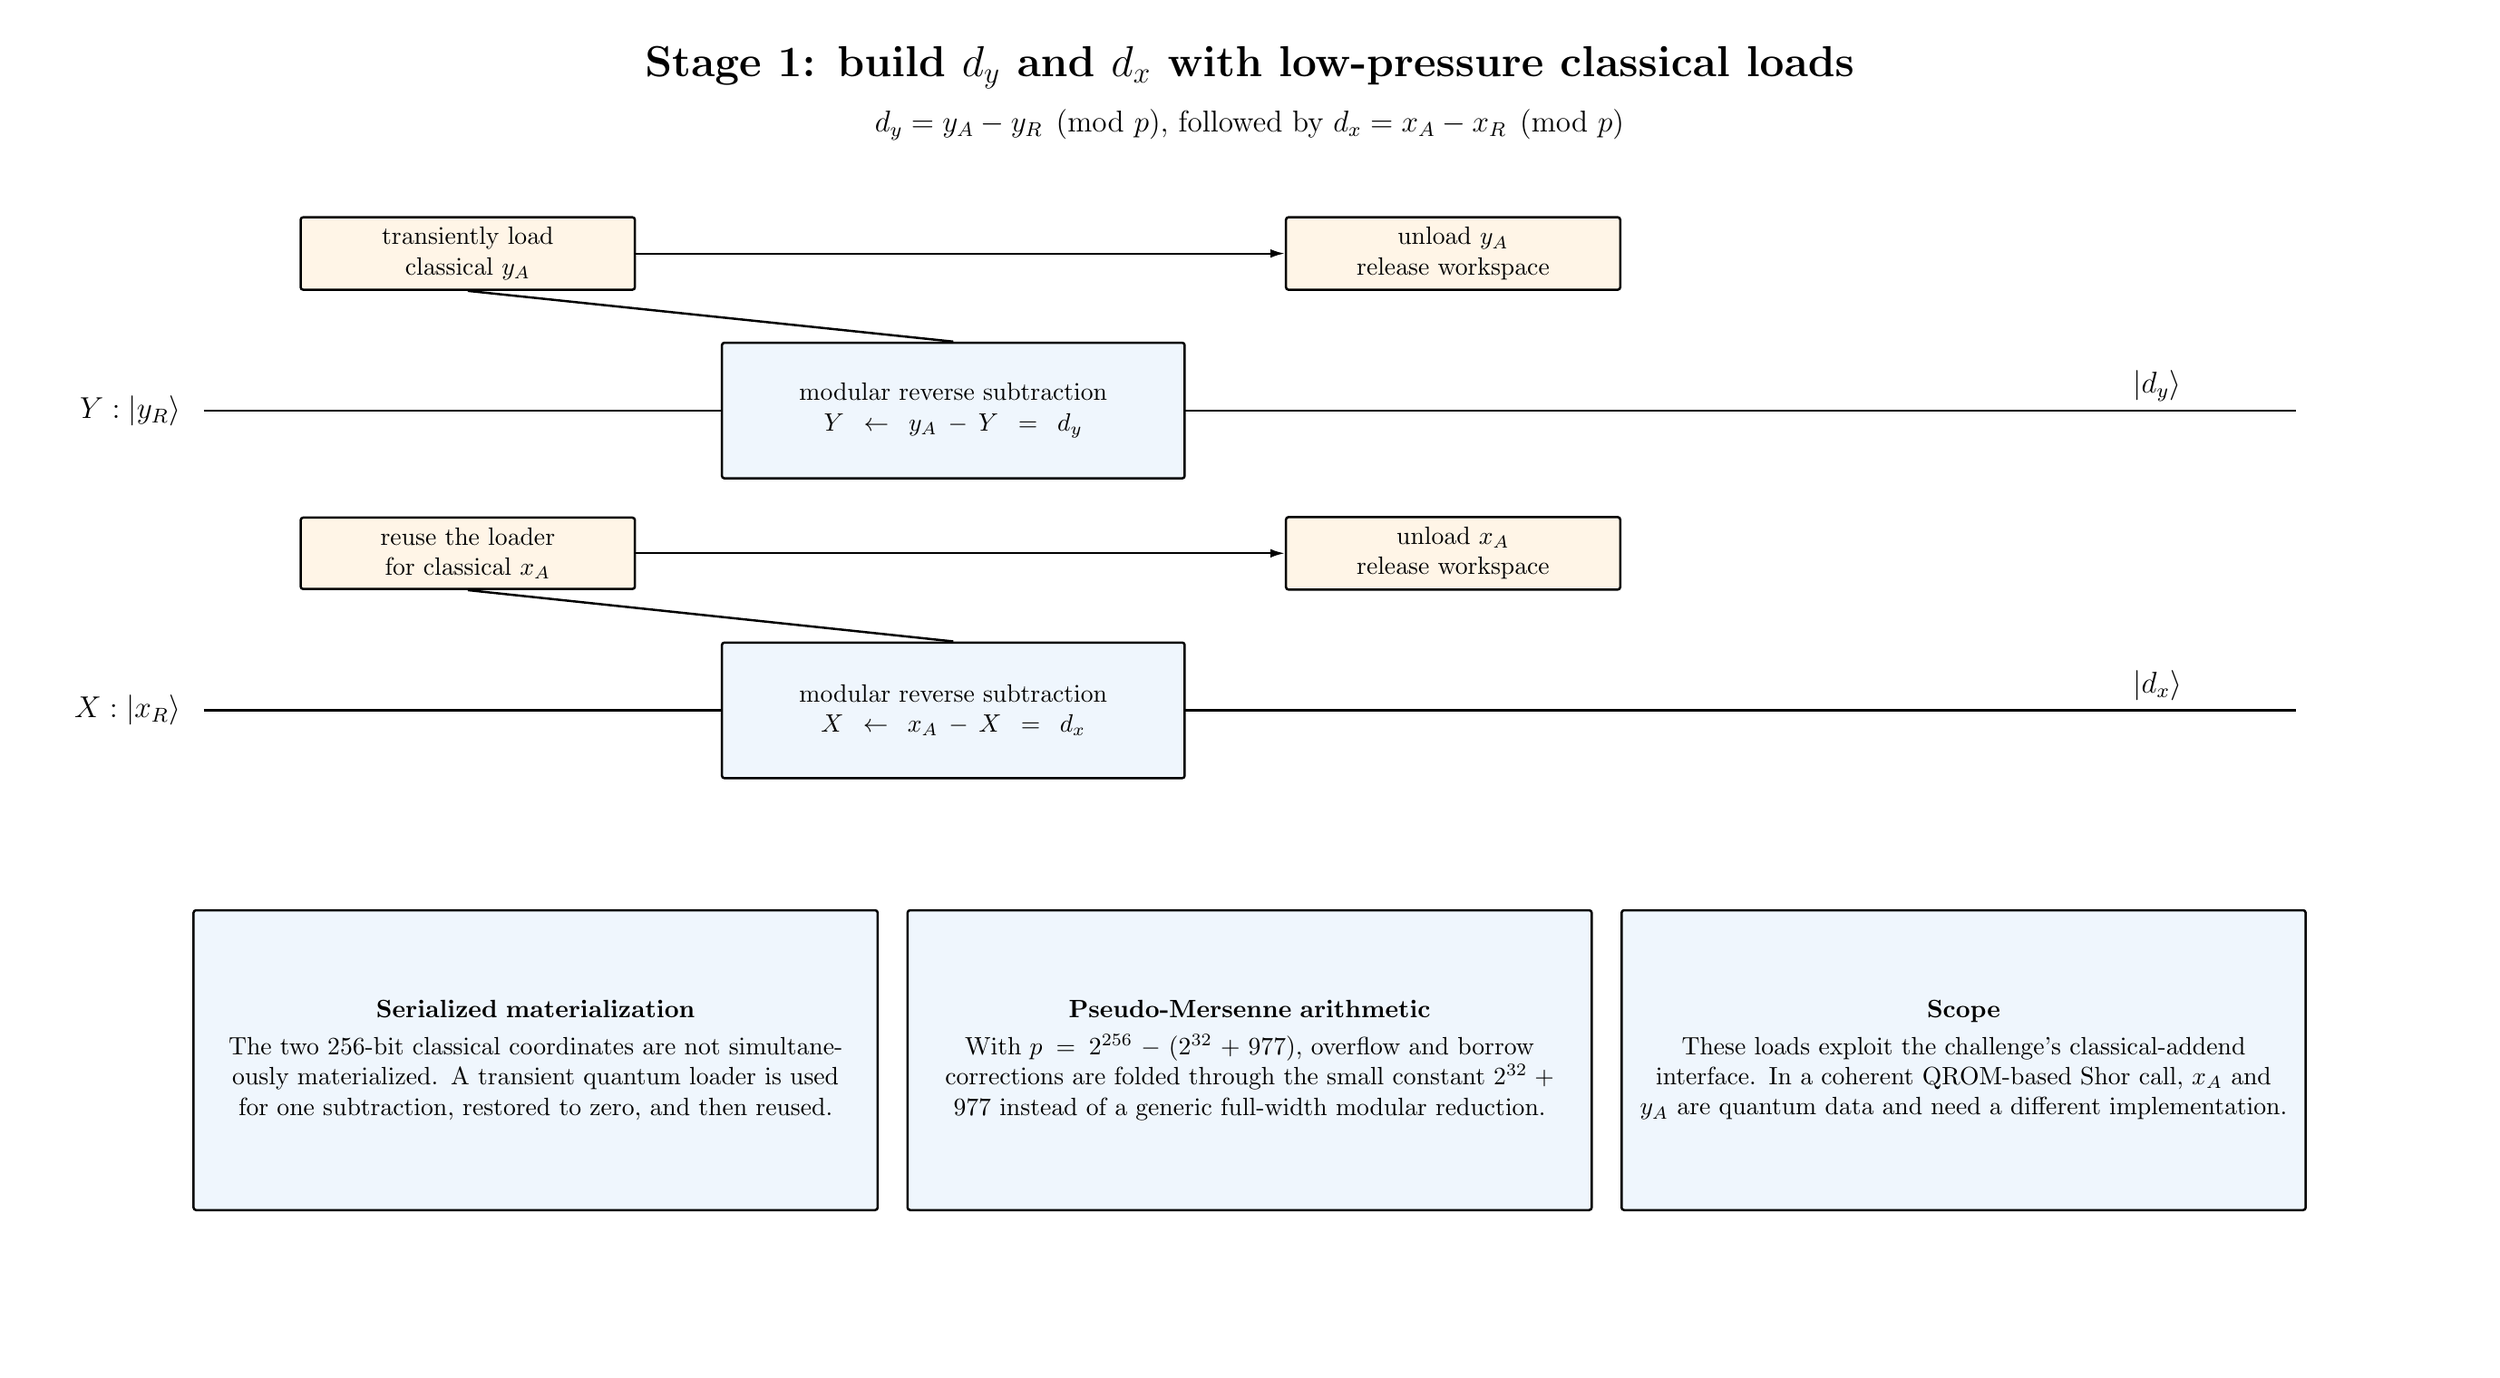
\begin{tikzpicture}[x=1cm,y=1cm]
  \path[use as bounding box] (0,0) rectangle (34.3,18.6);
  \node[font=\LARGE\bfseries] at (17.15,18.0)
    {Stage 1: build $d_y$ and $d_x$ with low-pressure classical loads};
  \node[font=\large] at (17.15,17.2)
    {$d_y=y_A-y_R\pmod p$, followed by $d_x=x_A-x_R\pmod p$};

  \node[lab,anchor=east] at (2.3,13.2) {$Y:\ket{y_R}$};
  \draw[wire] (2.5,13.2) -- (31.8,13.2);
  \node[classical,text width=44mm] (LY) at (6.2,15.4) {transiently load\\classical $y_A$};
  \node[gate,text width=62mm,minimum height=19mm] (SY) at (13.0,13.2)
    {modular reverse subtraction\\$Y\gets y_A-Y=d_y$};
  \node[classical,text width=44mm] (UY) at (20.0,15.4) {unload $y_A$\\release workspace};
  \draw[wire] (LY.south) -- (SY.north);
  \draw[flow] (LY.east) -- (UY.west);
  \node[lab,anchor=west] at (29.4,13.55) {$\ket{d_y}$};

  \node[lab,anchor=east] at (2.3,9.0) {$X:\ket{x_R}$};
  \draw[wire] (2.5,9.0) -- (31.8,9.0);
  \node[classical,text width=44mm] (LX) at (6.2,11.2) {reuse the loader\\for classical $x_A$};
  \node[gate,text width=62mm,minimum height=19mm] (SX) at (13.0,9.0)
    {modular reverse subtraction\\$X\gets x_A-X=d_x$};
  \node[classical,text width=44mm] (UX) at (20.0,11.2) {unload $x_A$\\release workspace};
  \draw[wire] (LX.south) -- (SX.north);
  \draw[flow] (LX.east) -- (UX.west);
  \node[lab,anchor=west] at (29.4,9.35) {$\ket{d_x}$};

  \node[detail,text width=93mm,minimum height=42mm] at (7.15,4.1)
    {\textbf{Serialized materialization}\\[1mm]
     The two $256$-bit classical coordinates are not simultaneously materialized. A transient
     quantum loader is used for one subtraction, restored to zero, and then reused.};
  \node[detail,text width=93mm,minimum height=42mm] at (17.15,4.1)
    {\textbf{Pseudo-Mersenne arithmetic}\\[1mm]
     With $p=2^{256}-(2^{32}+977)$, overflow and borrow corrections are folded through
     the small constant $2^{32}+977$ instead of a generic full-width modular reduction.};
  \node[detail,text width=93mm,minimum height=42mm] at (27.15,4.1)
    {\textbf{Scope}\\[1mm]
     These loads exploit the challenge's classical-addend interface. In a coherent QROM-based
     Shor call, $x_A$ and $y_A$ are quantum data and need a different implementation.};
\end{tikzpicture}
\newpage

% ============================================================================
% Additional analysis: low-pressure modular arithmetic
% ============================================================================
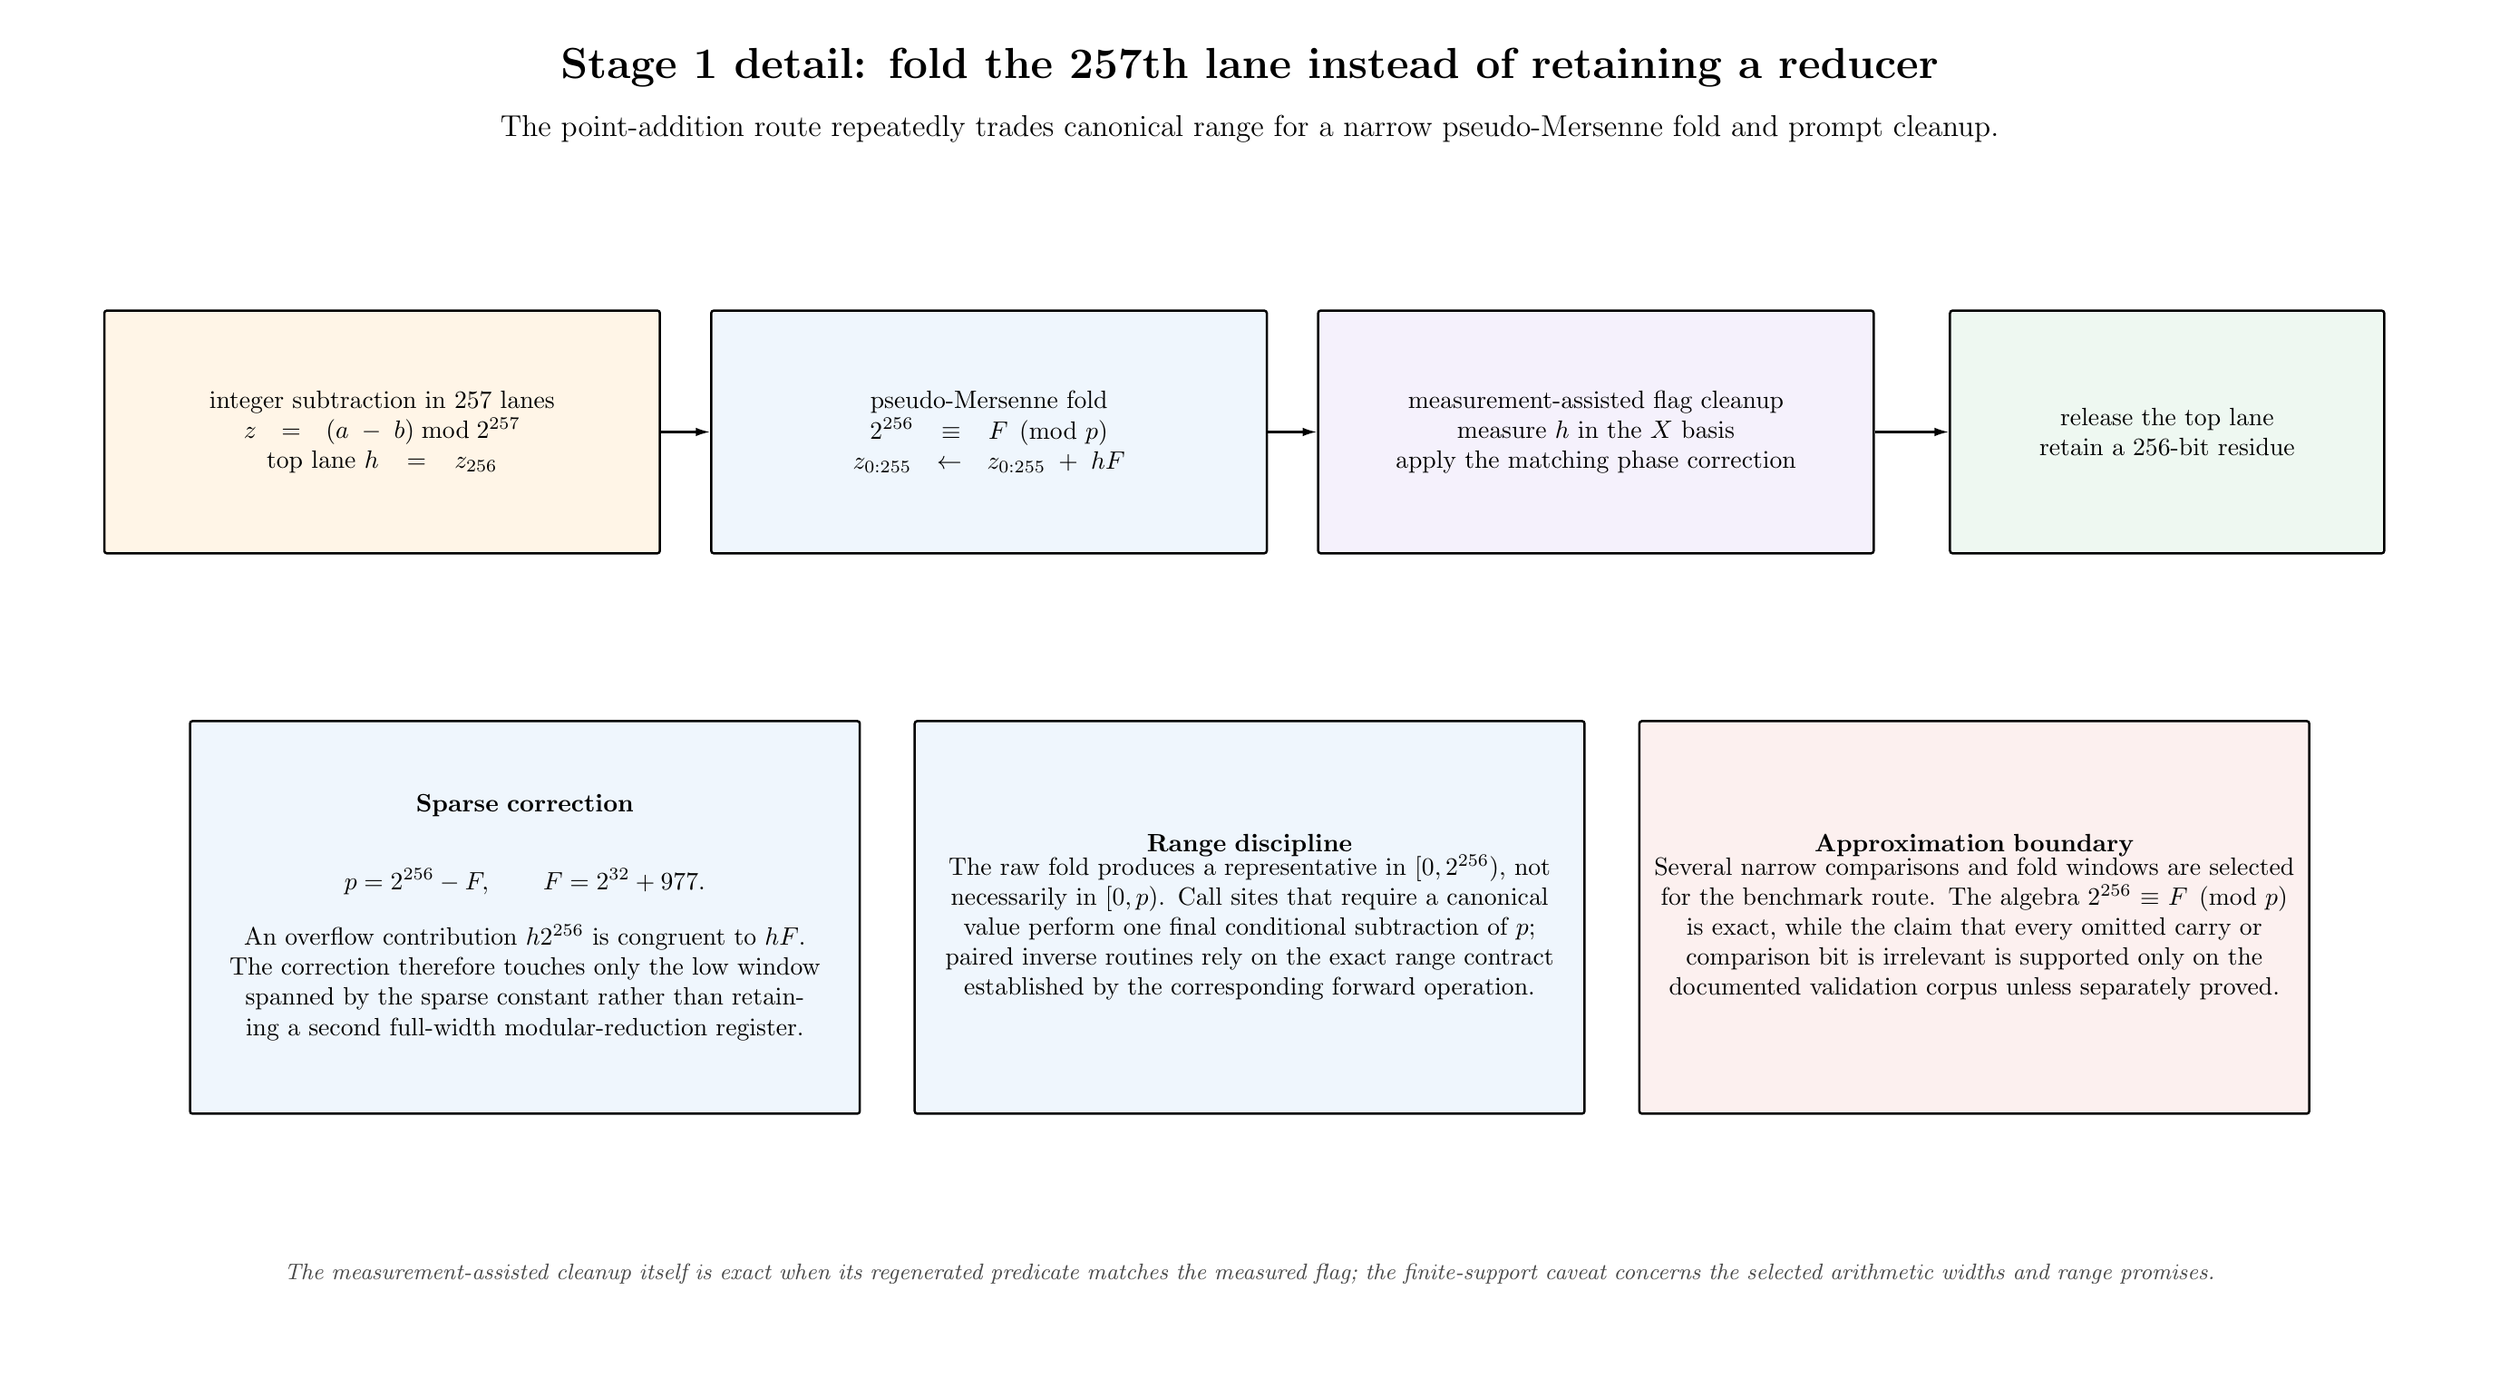
\begin{tikzpicture}[x=1cm,y=1cm]
  \path[use as bounding box] (0,0) rectangle (34.3,18.6);
  \node[font=\LARGE\bfseries] at (17.15,18.0)
    {Stage 1 detail: fold the 257th lane instead of retaining a reducer};
  \node[font=\large] at (17.15,17.15)
    {The point-addition route repeatedly trades canonical range for a narrow pseudo-Mersenne fold and prompt cleanup.};

  \node[classical,text width=75mm,minimum height=34mm] (SUB) at (5.0,12.9)
    {integer subtraction in $257$ lanes\\
     $z=(a-b)\bmod 2^{257}$\\
     top lane $h=z_{256}$};
  \node[gate,text width=75mm,minimum height=34mm] (FOLD) at (13.5,12.9)
    {pseudo-Mersenne fold\\
     $2^{256}\equiv F\pmod p$\\
     $z_{0:255}\gets z_{0:255}+hF$};
  \node[inversion,text width=75mm,minimum height=34mm] (MBU) at (22.0,12.9)
    {measurement-assisted flag cleanup\\
     measure $h$ in the $X$ basis\\
     apply the matching phase correction};
  \node[result,text width=58mm,minimum height=34mm] (OUTR) at (30.0,12.9)
    {release the top lane\\retain a $256$-bit residue};
  \draw[flow] (SUB.east)--(FOLD.west);
  \draw[flow] (FOLD.east)--(MBU.west);
  \draw[flow] (MBU.east)--(OUTR.west);

  \node[detail,text width=91mm,minimum height=55mm] at (7.0,6.1)
    {\textbf{Sparse correction}\\[-1mm]
     \[
       p=2^{256}-F,\qquad F=2^{32}+977.
     \]
     An overflow contribution $h2^{256}$ is congruent to $hF$. The correction therefore touches
     only the low window spanned by the sparse constant rather than retaining a second full-width
     modular-reduction register.};
  \node[detail,text width=91mm,minimum height=55mm] at (17.15,6.1)
    {\textbf{Range discipline}\\[-1mm]
     The raw fold produces a representative in $[0,2^{256})$, not necessarily in $[0,p)$.
     Call sites that require a canonical value perform one final conditional subtraction of $p$;
     paired inverse routines rely on the exact range contract established by the corresponding
     forward operation.};
  \node[warning,text width=91mm,minimum height=55mm] at (27.3,6.1)
    {\textbf{Approximation boundary}\\[-1mm]
     Several narrow comparisons and fold windows are selected for the benchmark route. The algebra
     $2^{256}\equiv F\pmod p$ is exact, while the claim that every omitted carry or comparison bit is
     irrelevant is supported only on the documented validation corpus unless separately proved.};

  \node[note,text width=30cm,align=center,font=\small\itshape] at (17.15,1.1)
    {The measurement-assisted cleanup itself is exact when its regenerated predicate matches the measured flag; the finite-support caveat concerns the selected arithmetic widths and range promises.};
\end{tikzpicture}
\newpage

% ============================================================================
% Page 6
% ============================================================================
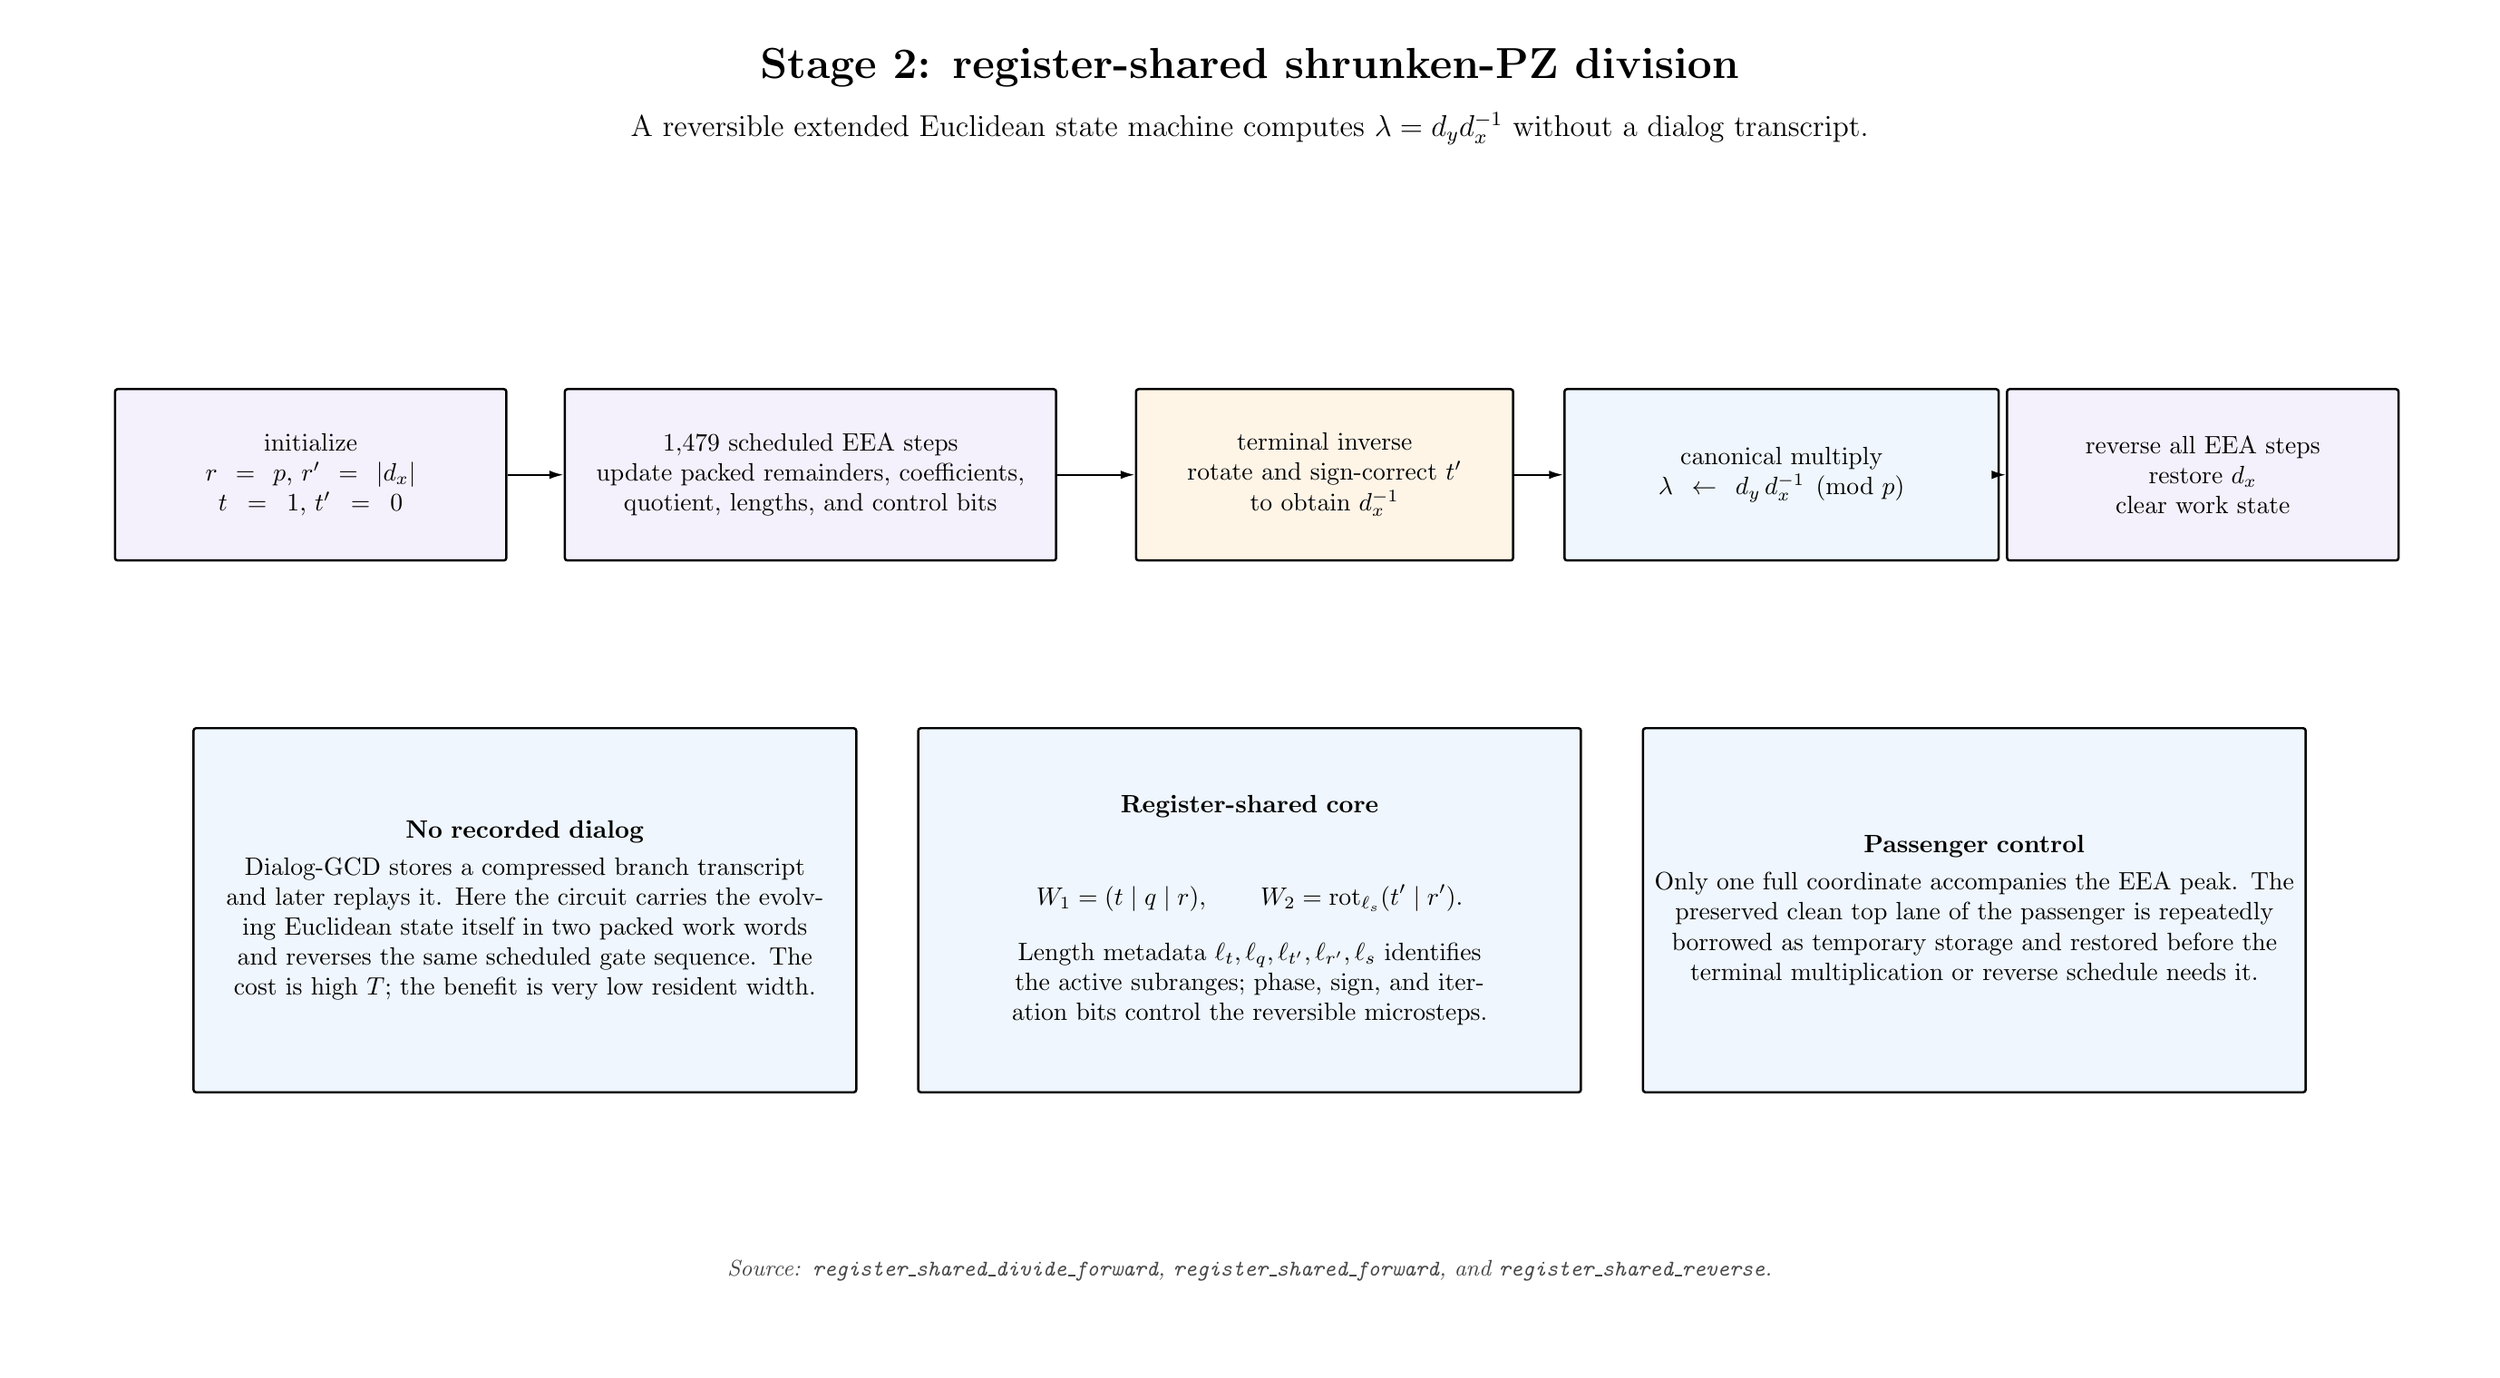
\begin{tikzpicture}[x=1cm,y=1cm]
  \path[use as bounding box] (0,0) rectangle (34.3,18.6);
  \node[font=\LARGE\bfseries] at (17.15,18.0)
    {Stage 2: register-shared shrunken-PZ division};
  \node[font=\large] at (17.15,17.15)
    {A reversible extended Euclidean state machine computes $\lambda=d_y d_x^{-1}$ without a dialog transcript.};

  \node[inversion,text width=52mm,minimum height=24mm] (INIT) at (4.0,12.3)
    {initialize\\$r=p$, $r'=|d_x|$\\$t=1$, $t'=0$};
  \node[inversion,text width=66mm,minimum height=24mm] (FWD) at (11.0,12.3)
    {$1{,}479$ scheduled EEA steps\\update packed remainders, coefficients,\\quotient, lengths, and control bits};
  \node[classical,text width=50mm,minimum height=24mm] (TERM) at (18.2,12.3)
    {terminal inverse\\rotate and sign-correct $t'$\\to obtain $d_x^{-1}$};
  \node[gate,text width=58mm,minimum height=24mm] (MUL) at (24.6,12.3)
    {canonical multiply\\$\lambda\gets d_y\,d_x^{-1}\pmod p$};
  \node[inversion,text width=52mm,minimum height=24mm] (REV) at (30.5,12.3)
    {reverse all EEA steps\\restore $d_x$\\clear work state};
  \draw[flow] (INIT.east) -- (FWD.west);
  \draw[flow] (FWD.east) -- (TERM.west);
  \draw[flow] (TERM.east) -- (MUL.west);
  \draw[flow] (MUL.east) -- (REV.west);

  \node[detail,text width=90mm,minimum height=51mm] at (7.0,6.2)
    {\textbf{No recorded dialog}\\[1mm]
     Dialog-GCD stores a compressed branch transcript and later replays it. Here the circuit carries
     the evolving Euclidean state itself in two packed work words and reverses the same scheduled
     gate sequence. The cost is high $T$; the benefit is very low resident width.};
  \node[detail,text width=90mm,minimum height=51mm] at (17.15,6.2)
    {\textbf{Register-shared core}\\[1mm]
     \[
       W_1=(t\mid q\mid r),\qquad W_2=\operatorname{rot}_{\ell_s}(t'\mid r').
     \]
     Length metadata $\ell_t,\ell_q,\ell_{t'},\ell_{r'},\ell_s$ identifies the active subranges;
     phase, sign, and iteration bits control the reversible microsteps.};
  \node[detail,text width=90mm,minimum height=51mm] at (27.3,6.2)
    {\textbf{Passenger control}\\[1mm]
     Only one full coordinate accompanies the EEA peak. The preserved clean top lane of the
     passenger is repeatedly borrowed as temporary storage and restored before the terminal
     multiplication or reverse schedule needs it.};

  \node[note,text width=30cm,align=center,font=\small\itshape] at (17.15,1.15)
    {Source: \texttt{register\_shared\_divide\_forward}, \texttt{register\_shared\_forward}, and \texttt{register\_shared\_reverse}.};
\end{tikzpicture}
\newpage

% ============================================================================
% Page 7
% ============================================================================
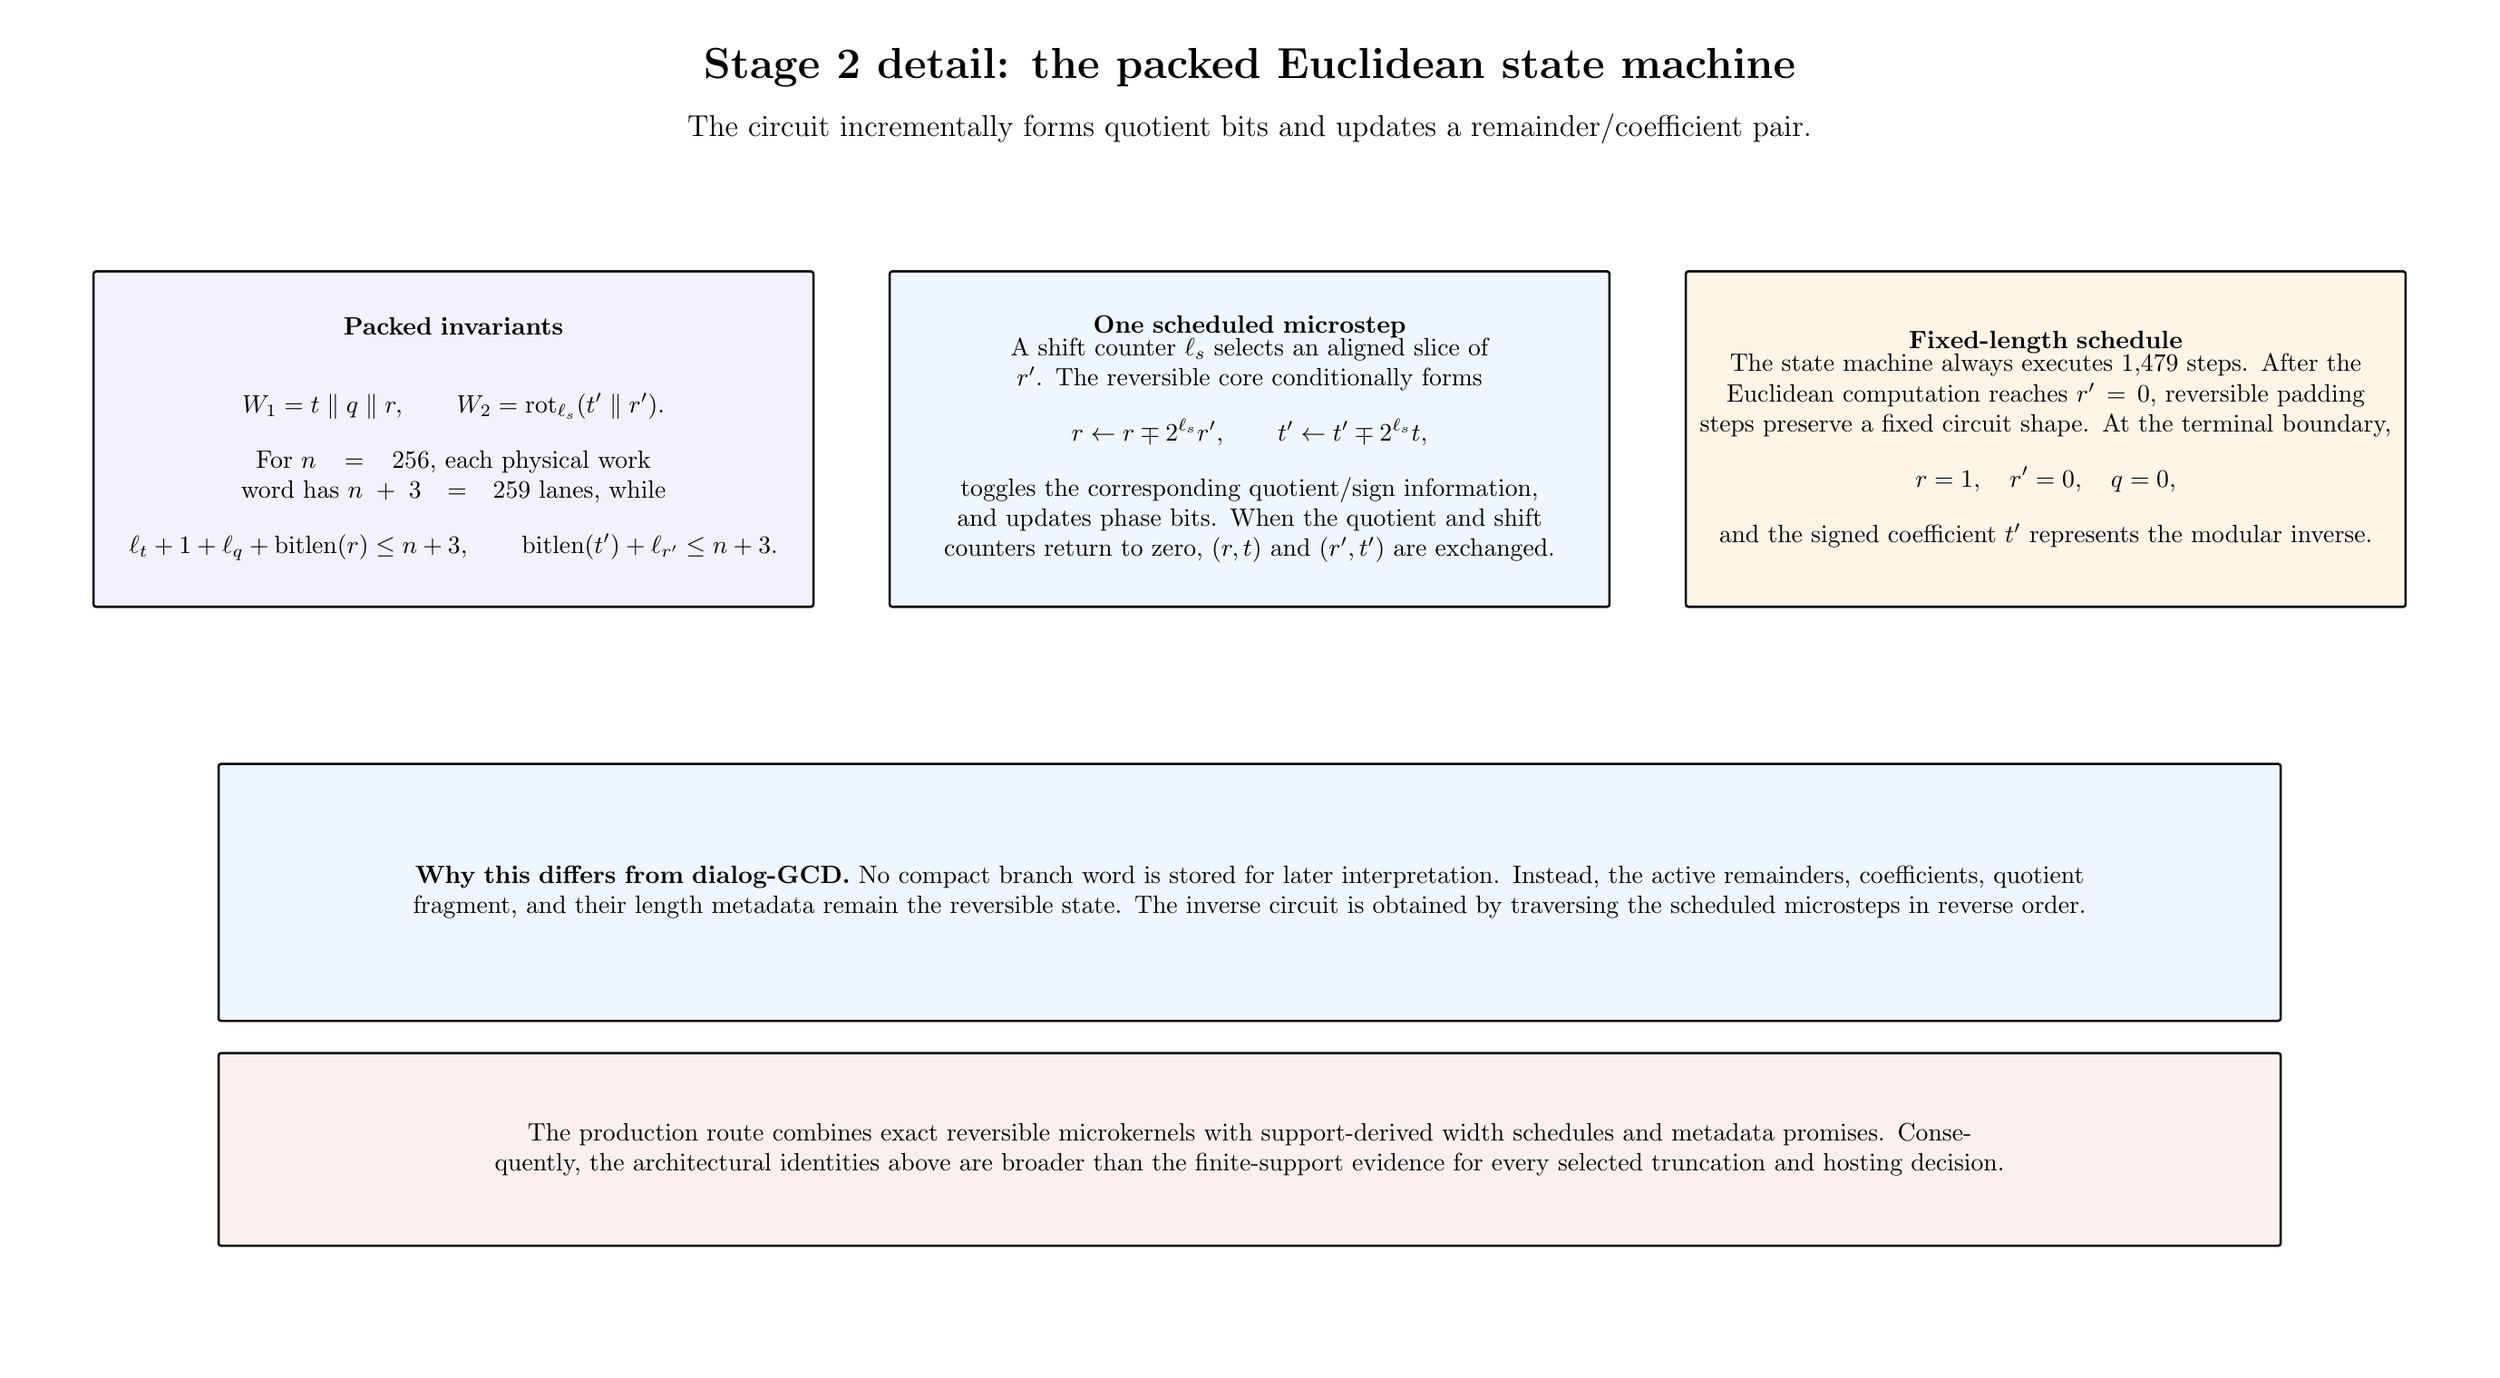
\begin{tikzpicture}[x=1cm,y=1cm]
  \path[use as bounding box] (0,0) rectangle (34.3,18.6);
  \node[font=\LARGE\bfseries] at (17.15,18.0)
    {Stage 2 detail: the packed Euclidean state machine};
  \node[font=\large] at (17.15,17.15)
    {The circuit incrementally forms quotient bits and updates a remainder/coefficient pair.};

  \node[inversion,text width=98mm,minimum height=47mm] at (6.0,12.8)
    {\textbf{Packed invariants}\\[-1mm]
     \[
       W_1=t\;\Vert\;q\;\Vert\;r,
       \qquad W_2=\operatorname{rot}_{\ell_s}(t'\;\Vert\;r').
     \]
     For $n=256$, each physical work word has $n+3=259$ lanes, while
     \[
       \ell_t+1+\ell_q+\operatorname{bitlen}(r)\le n+3,
       \qquad \operatorname{bitlen}(t')+\ell_{r'}\le n+3.
     \]};
  \node[detail,text width=98mm,minimum height=47mm] at (17.15,12.8)
    {\textbf{One scheduled microstep}\\[-1mm]
     A shift counter $\ell_s$ selects an aligned slice of $r'$. The reversible core conditionally forms
     \[
       r\leftarrow r\mp 2^{\ell_s}r',\qquad
       t'\leftarrow t'\mp 2^{\ell_s}t,
     \]
     toggles the corresponding quotient/sign information, and updates phase bits. When the quotient
     and shift counters return to zero, $(r,t)$ and $(r',t')$ are exchanged.};

  \node[classical,text width=98mm,minimum height=47mm] at (28.3,12.8)
    {\textbf{Fixed-length schedule}\\[-1mm]
     The state machine always executes $1{,}479$ steps. After the Euclidean computation reaches
     $r'=0$, reversible padding steps preserve a fixed circuit shape. At the terminal boundary,
     \[
       r=1,\quad r'=0,\quad q=0,
     \]
     and the signed coefficient $t'$ represents the modular inverse.};

  \node[detailwide,text width=286mm,minimum height=36mm] at (17.15,6.45)
    {\textbf{Why this differs from dialog-GCD.} No compact branch word is stored for later interpretation.
     Instead, the active remainders, coefficients, quotient fragment, and their length metadata remain the
     reversible state. The inverse circuit is obtained by traversing the scheduled microsteps in reverse order.};

  \node[warning,text width=286mm,minimum height=27mm] at (17.15,2.85)
    {The production route combines exact reversible microkernels with support-derived width schedules and
     metadata promises. Consequently, the architectural identities above are broader than the finite-support
     evidence for every selected truncation and hosting decision.};
\end{tikzpicture}
\newpage

% ============================================================================
% Additional analysis: reflected input, schedule, and terminal state
% ============================================================================
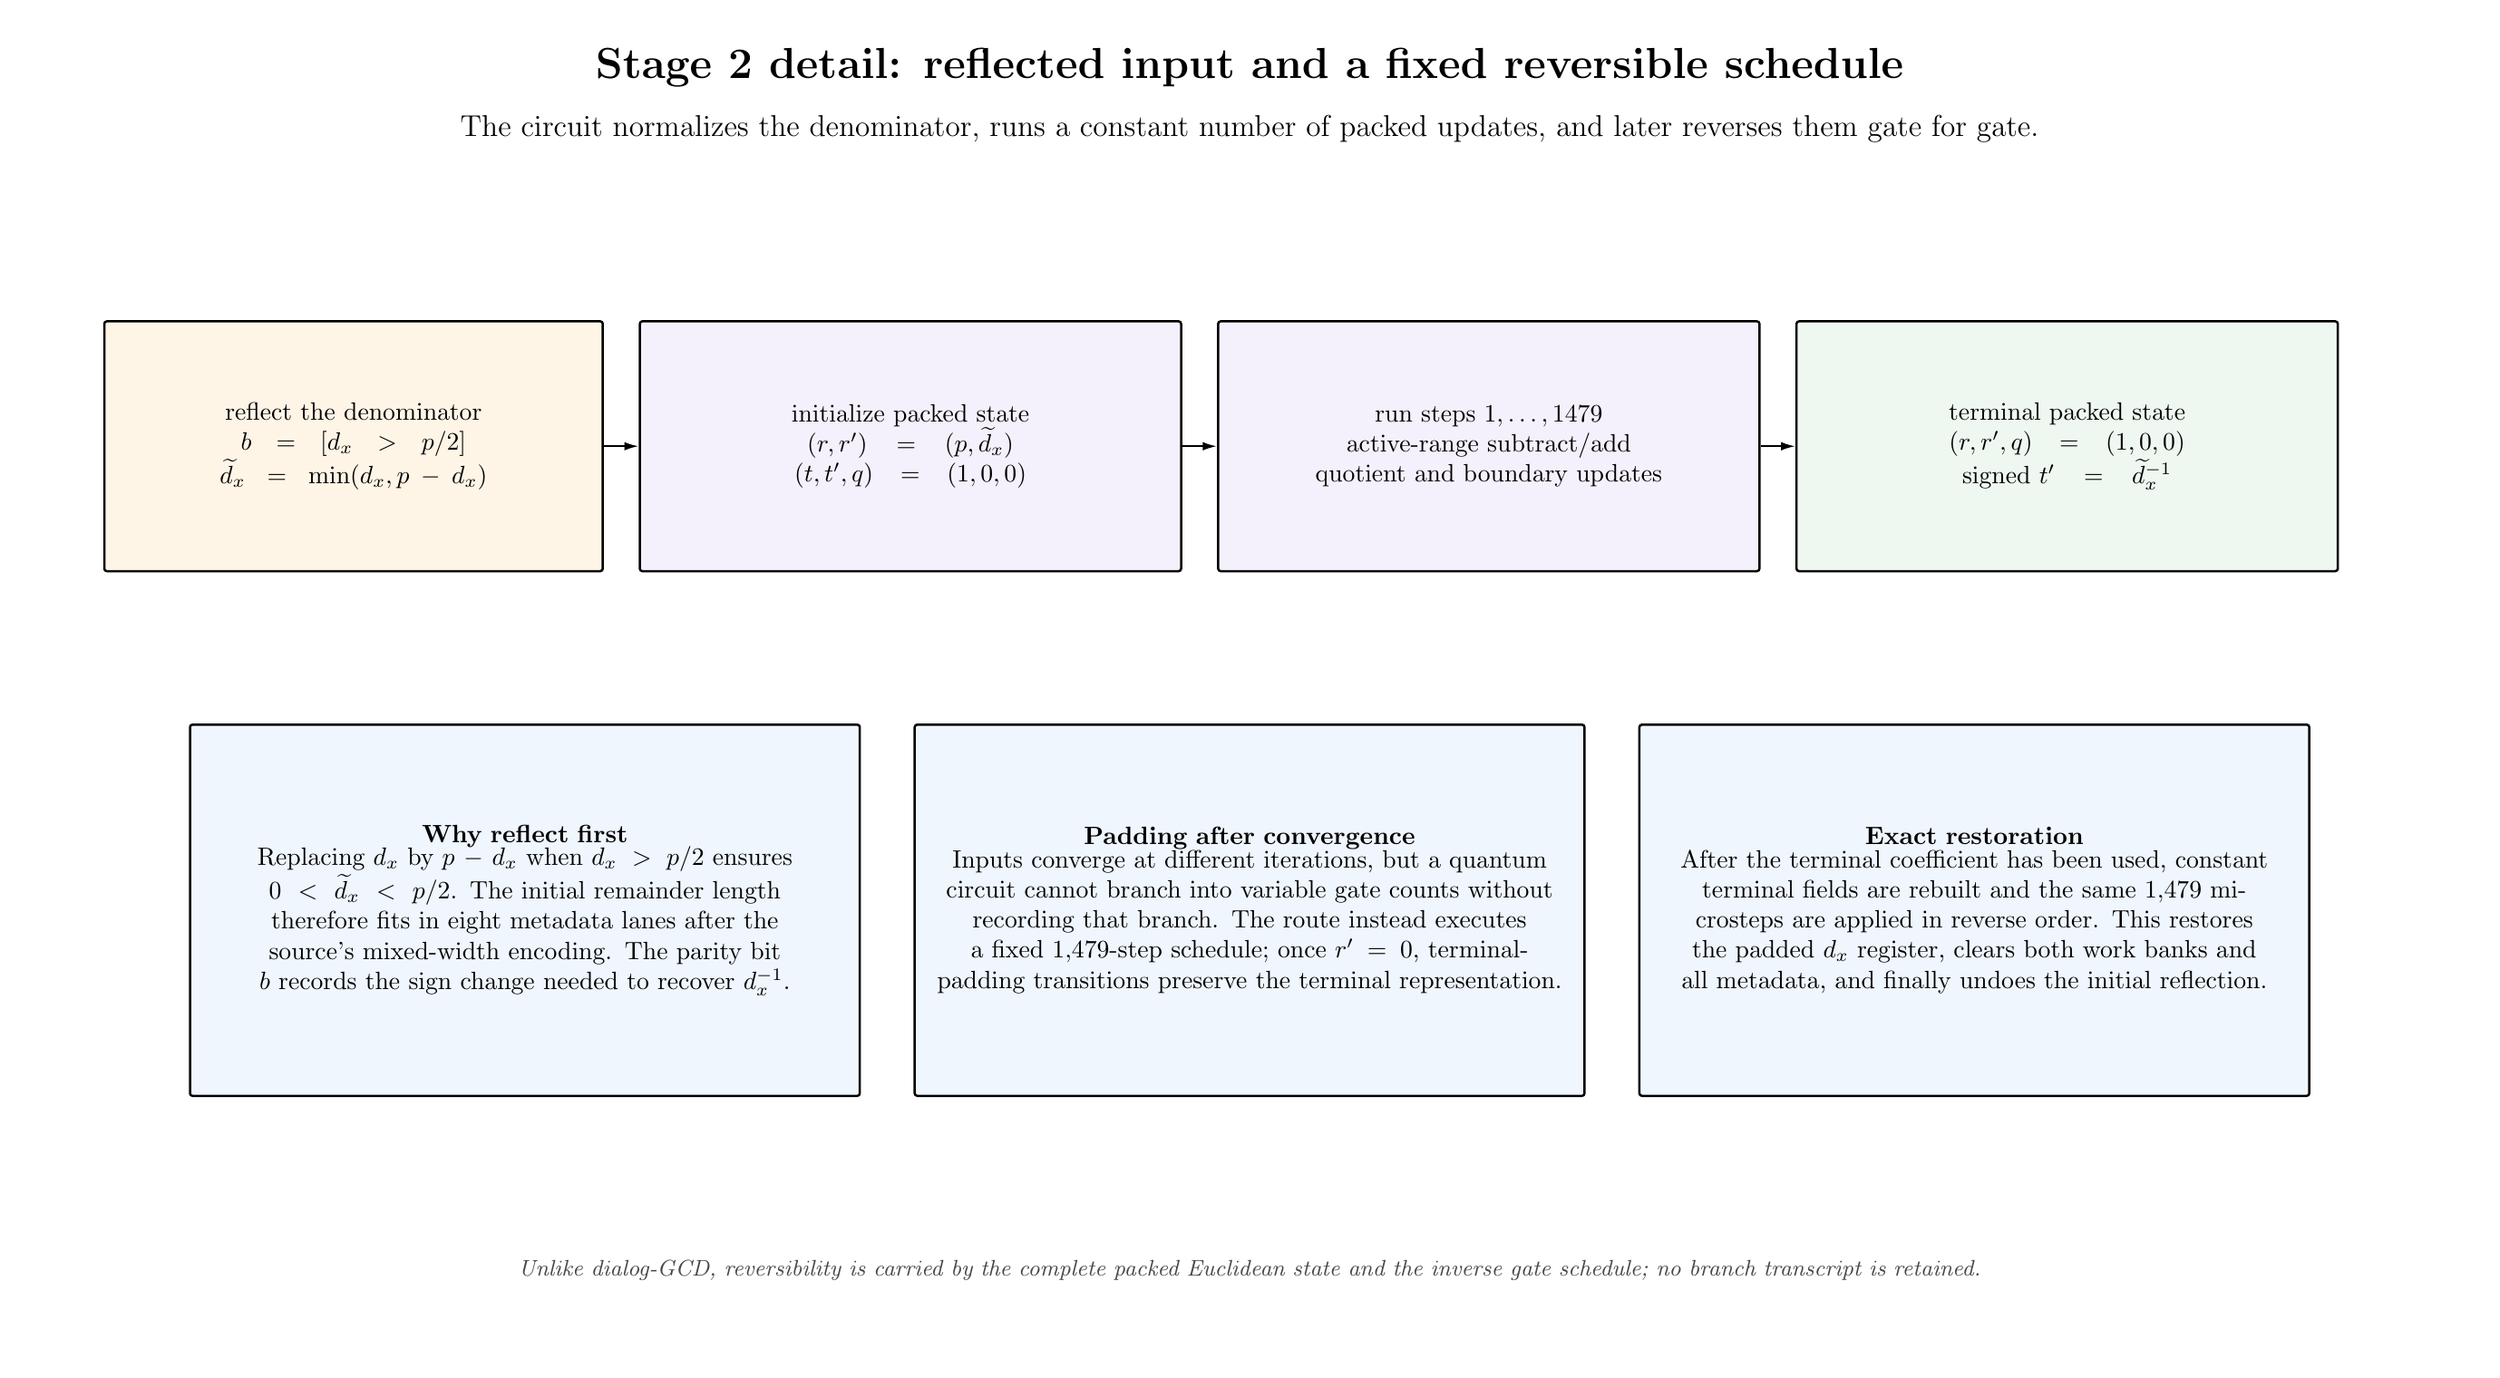
\begin{tikzpicture}[x=1cm,y=1cm]
  \path[use as bounding box] (0,0) rectangle (34.3,18.6);
  \node[font=\LARGE\bfseries] at (17.15,18.0)
    {Stage 2 detail: reflected input and a fixed reversible schedule};
  \node[font=\large] at (17.15,17.15)
    {The circuit normalizes the denominator, runs a constant number of packed updates, and later reverses them gate for gate.};

  \node[classical,text width=67mm,minimum height=35mm] (REF) at (4.6,12.7)
    {reflect the denominator\\
     $b=[d_x>p/2]$\\
     $\widetilde d_x=\min(d_x,p-d_x)$};
  \node[inversion,text width=73mm,minimum height=35mm] (INI) at (12.4,12.7)
    {initialize packed state\\
     $(r,r')=(p,\widetilde d_x)$\\
     $(t,t',q)=(1,0,0)$};
  \node[inversion,text width=73mm,minimum height=35mm] (SCH) at (20.5,12.7)
    {run steps $1,\ldots,1479$\\
     active-range subtract/add\\
     quotient and boundary updates};
  \node[result,text width=73mm,minimum height=35mm] (TER) at (28.6,12.7)
    {terminal packed state\\
     $(r,r',q)=(1,0,0)$\\
     signed $t'=\widetilde d_x^{-1}$};
  \draw[flow] (REF.east)--(INI.west);
  \draw[flow] (INI.east)--(SCH.west);
  \draw[flow] (SCH.east)--(TER.west);

  \node[detail,text width=91mm,minimum height=52mm] at (7.0,6.2)
    {\textbf{Why reflect first}\\[-1mm]
     Replacing $d_x$ by $p-d_x$ when $d_x>p/2$ ensures
     $0<\widetilde d_x<p/2$. The initial remainder length therefore fits in eight metadata
     lanes after the source's mixed-width encoding. The parity bit $b$ records the sign change
     needed to recover $d_x^{-1}$.};
  \node[detail,text width=91mm,minimum height=52mm] at (17.15,6.2)
    {\textbf{Padding after convergence}\\[-1mm]
     Inputs converge at different iterations, but a quantum circuit cannot branch into variable
     gate counts without recording that branch. The route instead executes a fixed $1{,}479$-step
     schedule; once $r'=0$, terminal-padding transitions preserve the terminal representation.};
  \node[detail,text width=91mm,minimum height=52mm] at (27.3,6.2)
    {\textbf{Exact restoration}\\[-1mm]
     After the terminal coefficient has been used, constant terminal fields are rebuilt and the
     same $1{,}479$ microsteps are applied in reverse order. This restores the padded $d_x$
     register, clears both work banks and all metadata, and finally undoes the initial reflection.};

  \node[note,text width=30cm,align=center,font=\small\itshape] at (17.15,1.15)
    {Unlike dialog-GCD, reversibility is carried by the complete packed Euclidean state and the inverse gate schedule; no branch transcript is retained.};
\end{tikzpicture}
\newpage

% ============================================================================
% Page 8
% ============================================================================
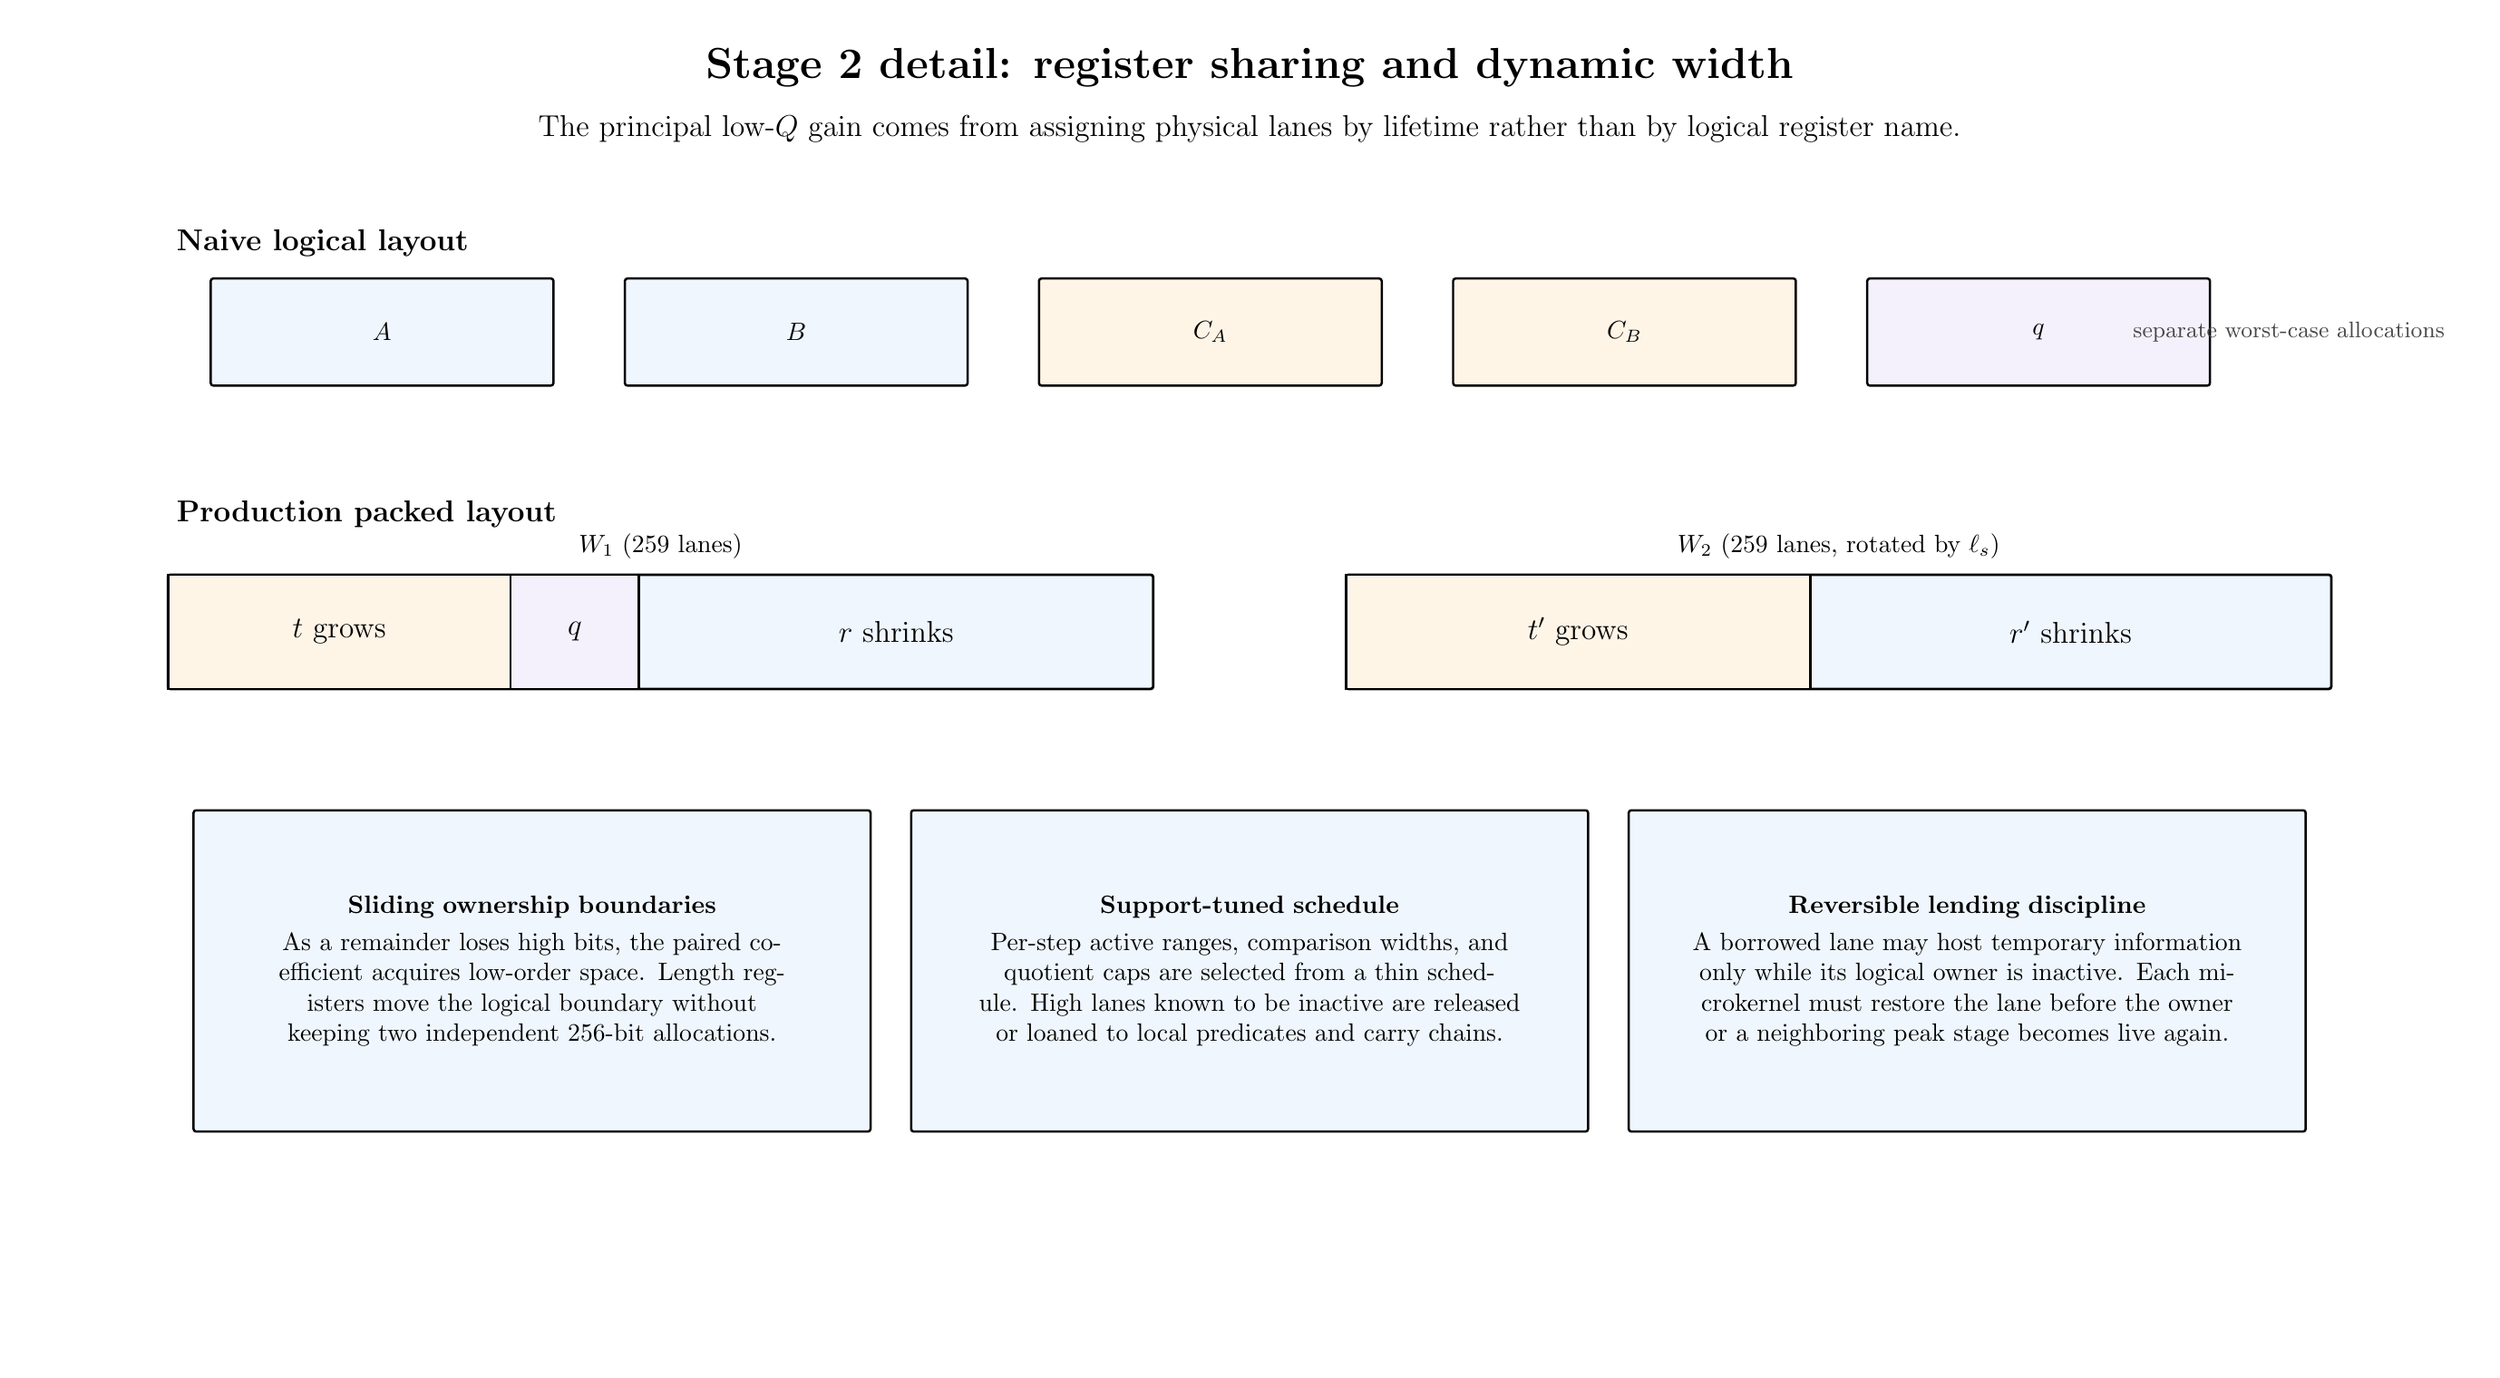
\begin{tikzpicture}[x=1cm,y=1cm]
  \path[use as bounding box] (0,0) rectangle (34.3,18.6);
  \node[font=\LARGE\bfseries] at (17.15,18.0)
    {Stage 2 detail: register sharing and dynamic width};
  \node[font=\large] at (17.15,17.15)
    {The principal low-$Q$ gain comes from assigning physical lanes by lifetime rather than by logical register name.};

  \node[font=\large\bfseries,anchor=west] at (2.0,15.55) {Naive logical layout};
  \foreach \x/\name/\shade in {3.3/A/gateblue,9.1/B/gateblue,14.9/C_A/lookorange,20.7/C_B/lookorange,26.5/q/invviolet}{
    \node[gate,fill=\shade,minimum width=48mm,minimum height=15mm] at (\x+1.7,14.3) {$\name$};
  }
  \node[note,anchor=west] at (29.4,14.3) {separate worst-case allocations};

  \node[font=\large\bfseries,anchor=west] at (2.0,11.75) {Production packed layout};
  \draw[black,line width=1pt,rounded corners=1pt,fill=gateblue] (2.0,9.3) rectangle (15.8,10.9);
  \draw[black,line width=1pt,fill=lookorange] (2.0,9.3) rectangle (6.8,10.9);
  \draw[black,line width=1pt,fill=invviolet] (6.8,9.3) rectangle (8.6,10.9);
  \node[font=\large] at (4.4,10.1) {$t$ grows};
  \node[font=\large] at (7.7,10.1) {$q$};
  \node[font=\large] at (12.2,10.1) {$r$ shrinks};
  \node[font=\normalsize,anchor=south] at (8.9,11.0) {$W_1$ (259 lanes)};

  \draw[black,line width=1pt,rounded corners=1pt,fill=gateblue] (18.5,9.3) rectangle (32.3,10.9);
  \draw[black,line width=1pt,fill=lookorange] (18.5,9.3) rectangle (25.0,10.9);
  \node[font=\large] at (21.75,10.1) {$t'$ grows};
  \node[font=\large] at (28.65,10.1) {$r'$ shrinks};
  \node[font=\normalsize,anchor=south] at (25.4,11.0) {$W_2$ (259 lanes, rotated by $\ell_s$)};

  \node[detail,text width=92mm,minimum height=45mm] at (7.1,5.35)
    {\textbf{Sliding ownership boundaries}\\[1mm]
     As a remainder loses high bits, the paired coefficient acquires low-order space. Length registers
     move the logical boundary without keeping two independent $256$-bit allocations.};
  \node[detail,text width=92mm,minimum height=45mm] at (17.15,5.35)
    {\textbf{Support-tuned schedule}\\[1mm]
     Per-step active ranges, comparison widths, and quotient caps are selected from a thin schedule.
     High lanes known to be inactive are released or loaned to local predicates and carry chains.};
  \node[detail,text width=92mm,minimum height=45mm] at (27.2,5.35)
    {\textbf{Reversible lending discipline}\\[1mm]
     A borrowed lane may host temporary information only while its logical owner is inactive. Each microkernel
     must restore the lane before the owner or a neighboring peak stage becomes live again.};
\end{tikzpicture}
\newpage

% ============================================================================
% Additional analysis: dynamic cursors
% ============================================================================
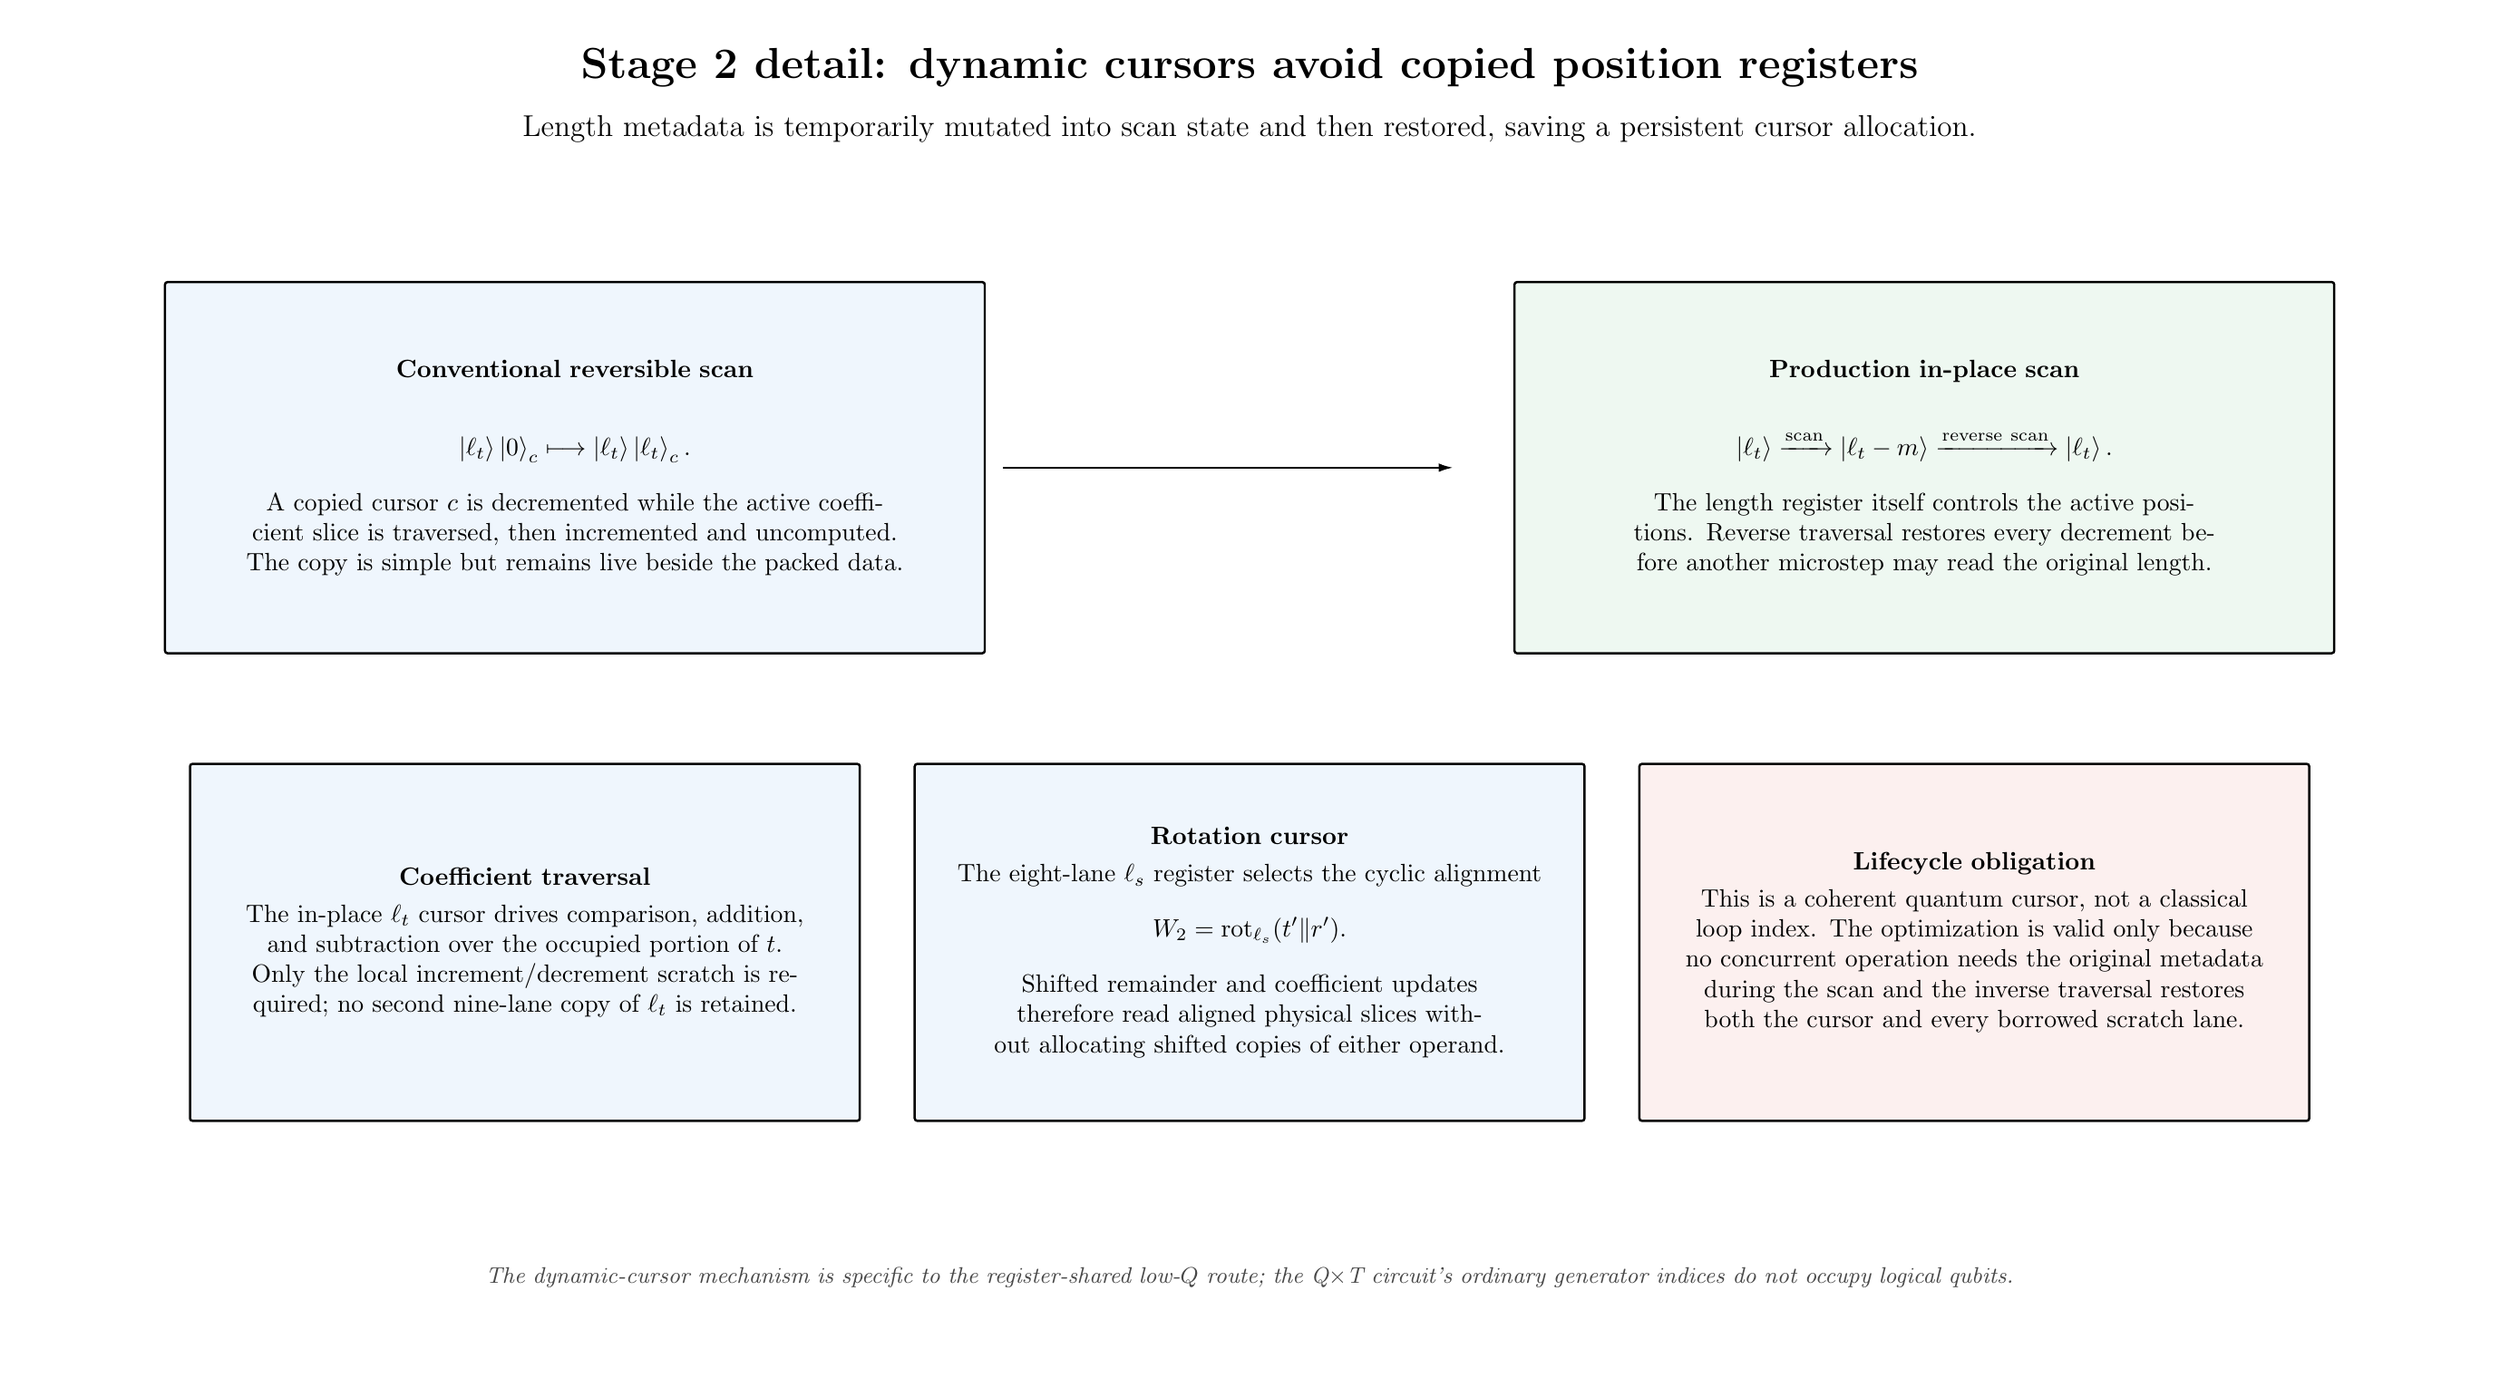
\begin{tikzpicture}[x=1cm,y=1cm]
  \path[use as bounding box] (0,0) rectangle (34.3,18.6);
  \node[font=\LARGE\bfseries] at (17.15,18.0)
    {Stage 2 detail: dynamic cursors avoid copied position registers};
  \node[font=\large] at (17.15,17.15)
    {Length metadata is temporarily mutated into scan state and then restored, saving a persistent cursor allocation.};

  \node[detail,text width=112mm,minimum height=52mm] at (7.7,12.4)
    {\textbf{Conventional reversible scan}\\[-1mm]
     \[
       \ket{\ell_t}\ket{0}_c
       \longmapsto \ket{\ell_t}\ket{\ell_t}_c.
     \]
     A copied cursor $c$ is decremented while the active coefficient slice is traversed, then
     incremented and uncomputed. The copy is simple but remains live beside the packed data.};
  \draw[flow] (13.7,12.4)--(20.0,12.4);
  \node[result,text width=112mm,minimum height=52mm] at (26.6,12.4)
    {\textbf{Production in-place scan}\\[-1mm]
     \[
       \ket{\ell_t}\xrightarrow{\rm scan}\ket{\ell_t-m}
       \xrightarrow{\rm reverse\ scan}\ket{\ell_t}.
     \]
     The length register itself controls the active positions. Reverse traversal restores every
     decrement before another microstep may read the original length.};

  \node[detail,text width=91mm,minimum height=50mm] at (7.0,5.75)
    {\textbf{Coefficient traversal}\\[1mm]
     The in-place $\ell_t$ cursor drives comparison, addition, and subtraction over the occupied
     portion of $t$. Only the local increment/decrement scratch is required; no second nine-lane
     copy of $\ell_t$ is retained.};
  \node[detail,text width=91mm,minimum height=50mm] at (17.15,5.75)
    {\textbf{Rotation cursor}\\[1mm]
     The eight-lane $\ell_s$ register selects the cyclic alignment
     \[
       W_2=\operatorname{rot}_{\ell_s}(t'\Vert r').
     \]
     Shifted remainder and coefficient updates therefore read aligned physical slices without
     allocating shifted copies of either operand.};
  \node[warning,text width=91mm,minimum height=50mm] at (27.3,5.75)
    {\textbf{Lifecycle obligation}\\[1mm]
     This is a coherent quantum cursor, not a classical loop index. The optimization is valid only
     because no concurrent operation needs the original metadata during the scan and the inverse
     traversal restores both the cursor and every borrowed scratch lane.};

  \node[note,text width=30cm,align=center,font=\small\itshape] at (17.15,1.05)
    {The dynamic-cursor mechanism is specific to the register-shared low-$Q$ route; the Q$\times$T circuit's ordinary generator indices do not occupy logical qubits.};
\end{tikzpicture}
\newpage

% ============================================================================
% Additional analysis: the Q826 host windows inherited by Q825
% ============================================================================
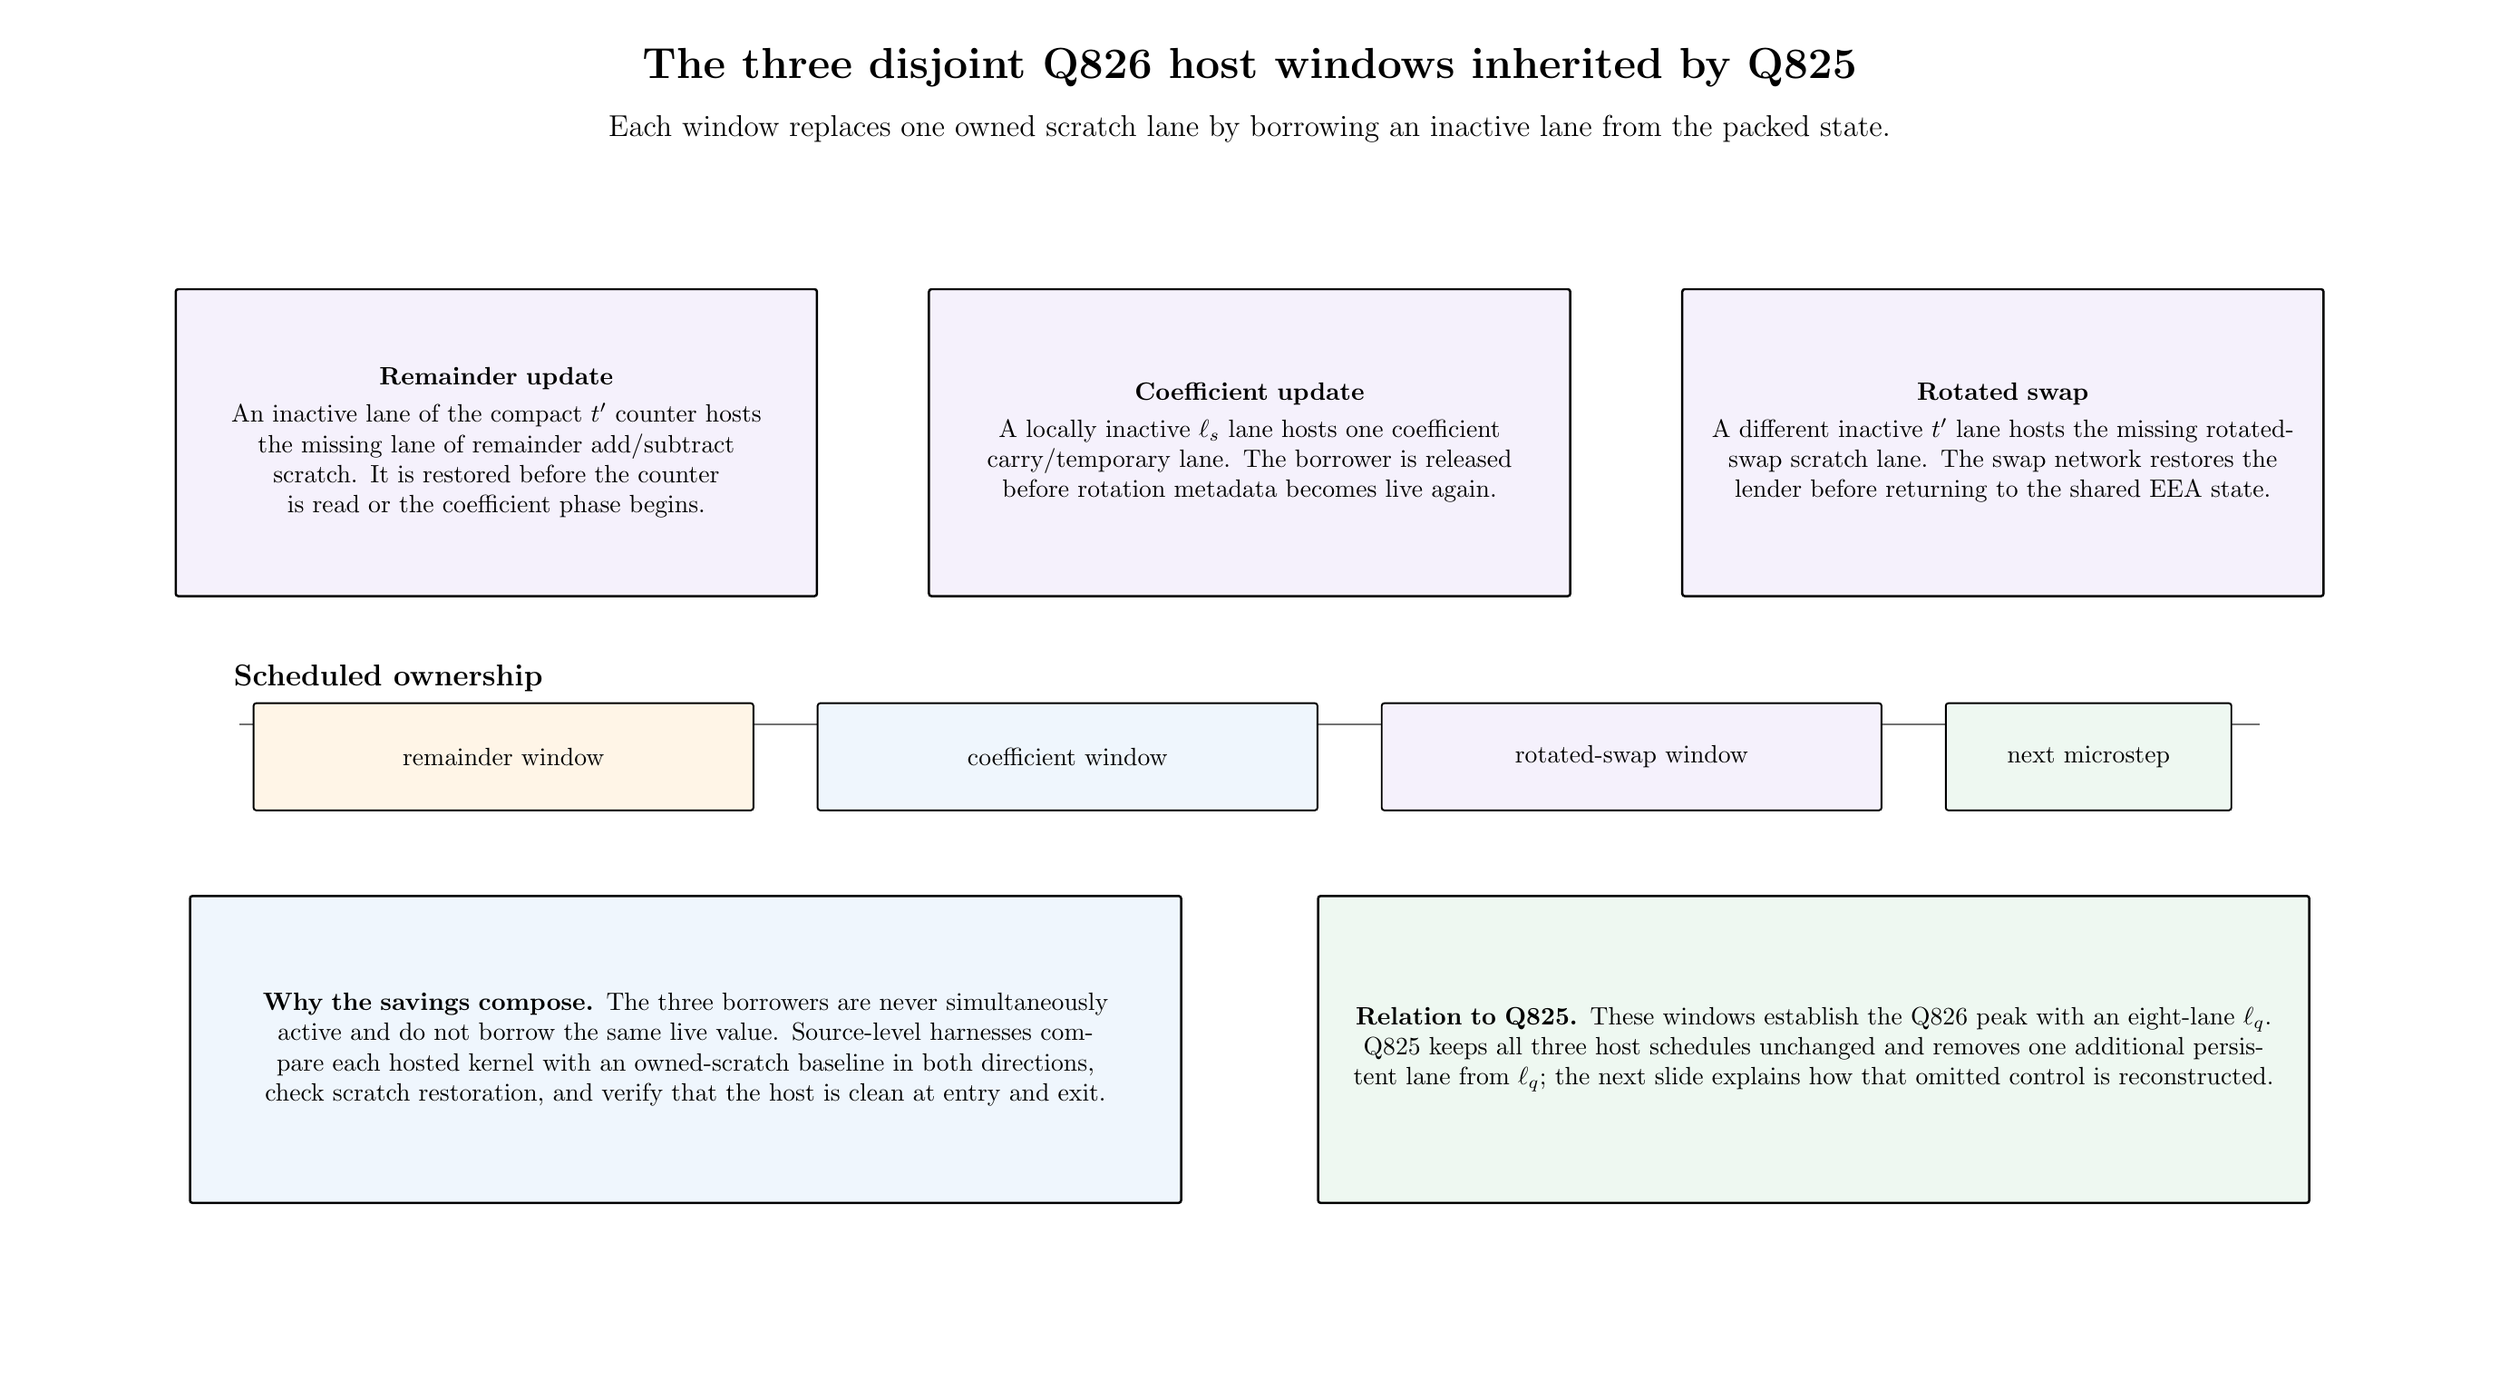
\begin{tikzpicture}[x=1cm,y=1cm]
  \path[use as bounding box] (0,0) rectangle (34.3,18.6);
  \node[font=\LARGE\bfseries] at (17.15,18.0)
    {The three disjoint Q826 host windows inherited by Q825};
  \node[font=\large] at (17.15,17.15)
    {Each window replaces one owned scratch lane by borrowing an inactive lane from the packed state.};

  \node[inversion,text width=87mm,minimum height=43mm] at (6.6,12.75)
    {\textbf{Remainder update}\\[1mm]
     An inactive lane of the compact $t'$ counter hosts the missing lane of remainder add/subtract
     scratch. It is restored before the counter is read or the coefficient phase begins.};
  \node[inversion,text width=87mm,minimum height=43mm] at (17.15,12.75)
    {\textbf{Coefficient update}\\[1mm]
     A locally inactive $\ell_s$ lane hosts one coefficient carry/temporary lane. The borrower is
     released before rotation metadata becomes live again.};
  \node[inversion,text width=87mm,minimum height=43mm] at (27.7,12.75)
    {\textbf{Rotated swap}\\[1mm]
     A different inactive $t'$ lane hosts the missing rotated-swap scratch lane. The swap network
     restores the lender before returning to the shared EEA state.};

  \draw[black!55,line width=0.8pt] (3.0,8.8)--(31.3,8.8);
  \node[font=\large\bfseries,anchor=west] at (2.8,9.45) {Scheduled ownership};
  \draw[black,line width=0.7pt,fill=lookorange,rounded corners=1pt] (3.2,7.6) rectangle ++(7.0,1.5);
  \node[font=\normalsize] at (6.7,8.35) {remainder window};
  \draw[black,line width=0.7pt,fill=gateblue,rounded corners=1pt] (11.1,7.6) rectangle ++(7.0,1.5);
  \node[font=\normalsize] at (14.6,8.35) {coefficient window};
  \draw[black,line width=0.7pt,fill=invviolet,rounded corners=1pt] (19.0,7.6) rectangle ++(7.0,1.5);
  \node[font=\normalsize] at (22.5,8.35) {rotated-swap window};
  \draw[black,line width=0.7pt,fill=outgreen,rounded corners=1pt] (26.9,7.6) rectangle ++(4.0,1.5);
  \node[font=\normalsize] at (28.9,8.35) {next microstep};

  \node[detail,text width=136mm,minimum height=43mm] at (9.25,4.25)
    {\textbf{Why the savings compose.} The three borrowers are never simultaneously active and do not
     borrow the same live value. Source-level harnesses compare each hosted kernel with an owned-scratch
     baseline in both directions, check scratch restoration, and verify that the host is clean at entry and exit.};
  \node[result,text width=136mm,minimum height=43mm] at (25.05,4.25)
    {\textbf{Relation to Q825.} These windows establish the Q826 peak with an eight-lane $\ell_q$.
     Q825 keeps all three host schedules unchanged and removes one additional persistent lane from
     $\ell_q$; the next slide explains how that omitted control is reconstructed.};
\end{tikzpicture}
\newpage

% ============================================================================
% Page 9
% ============================================================================
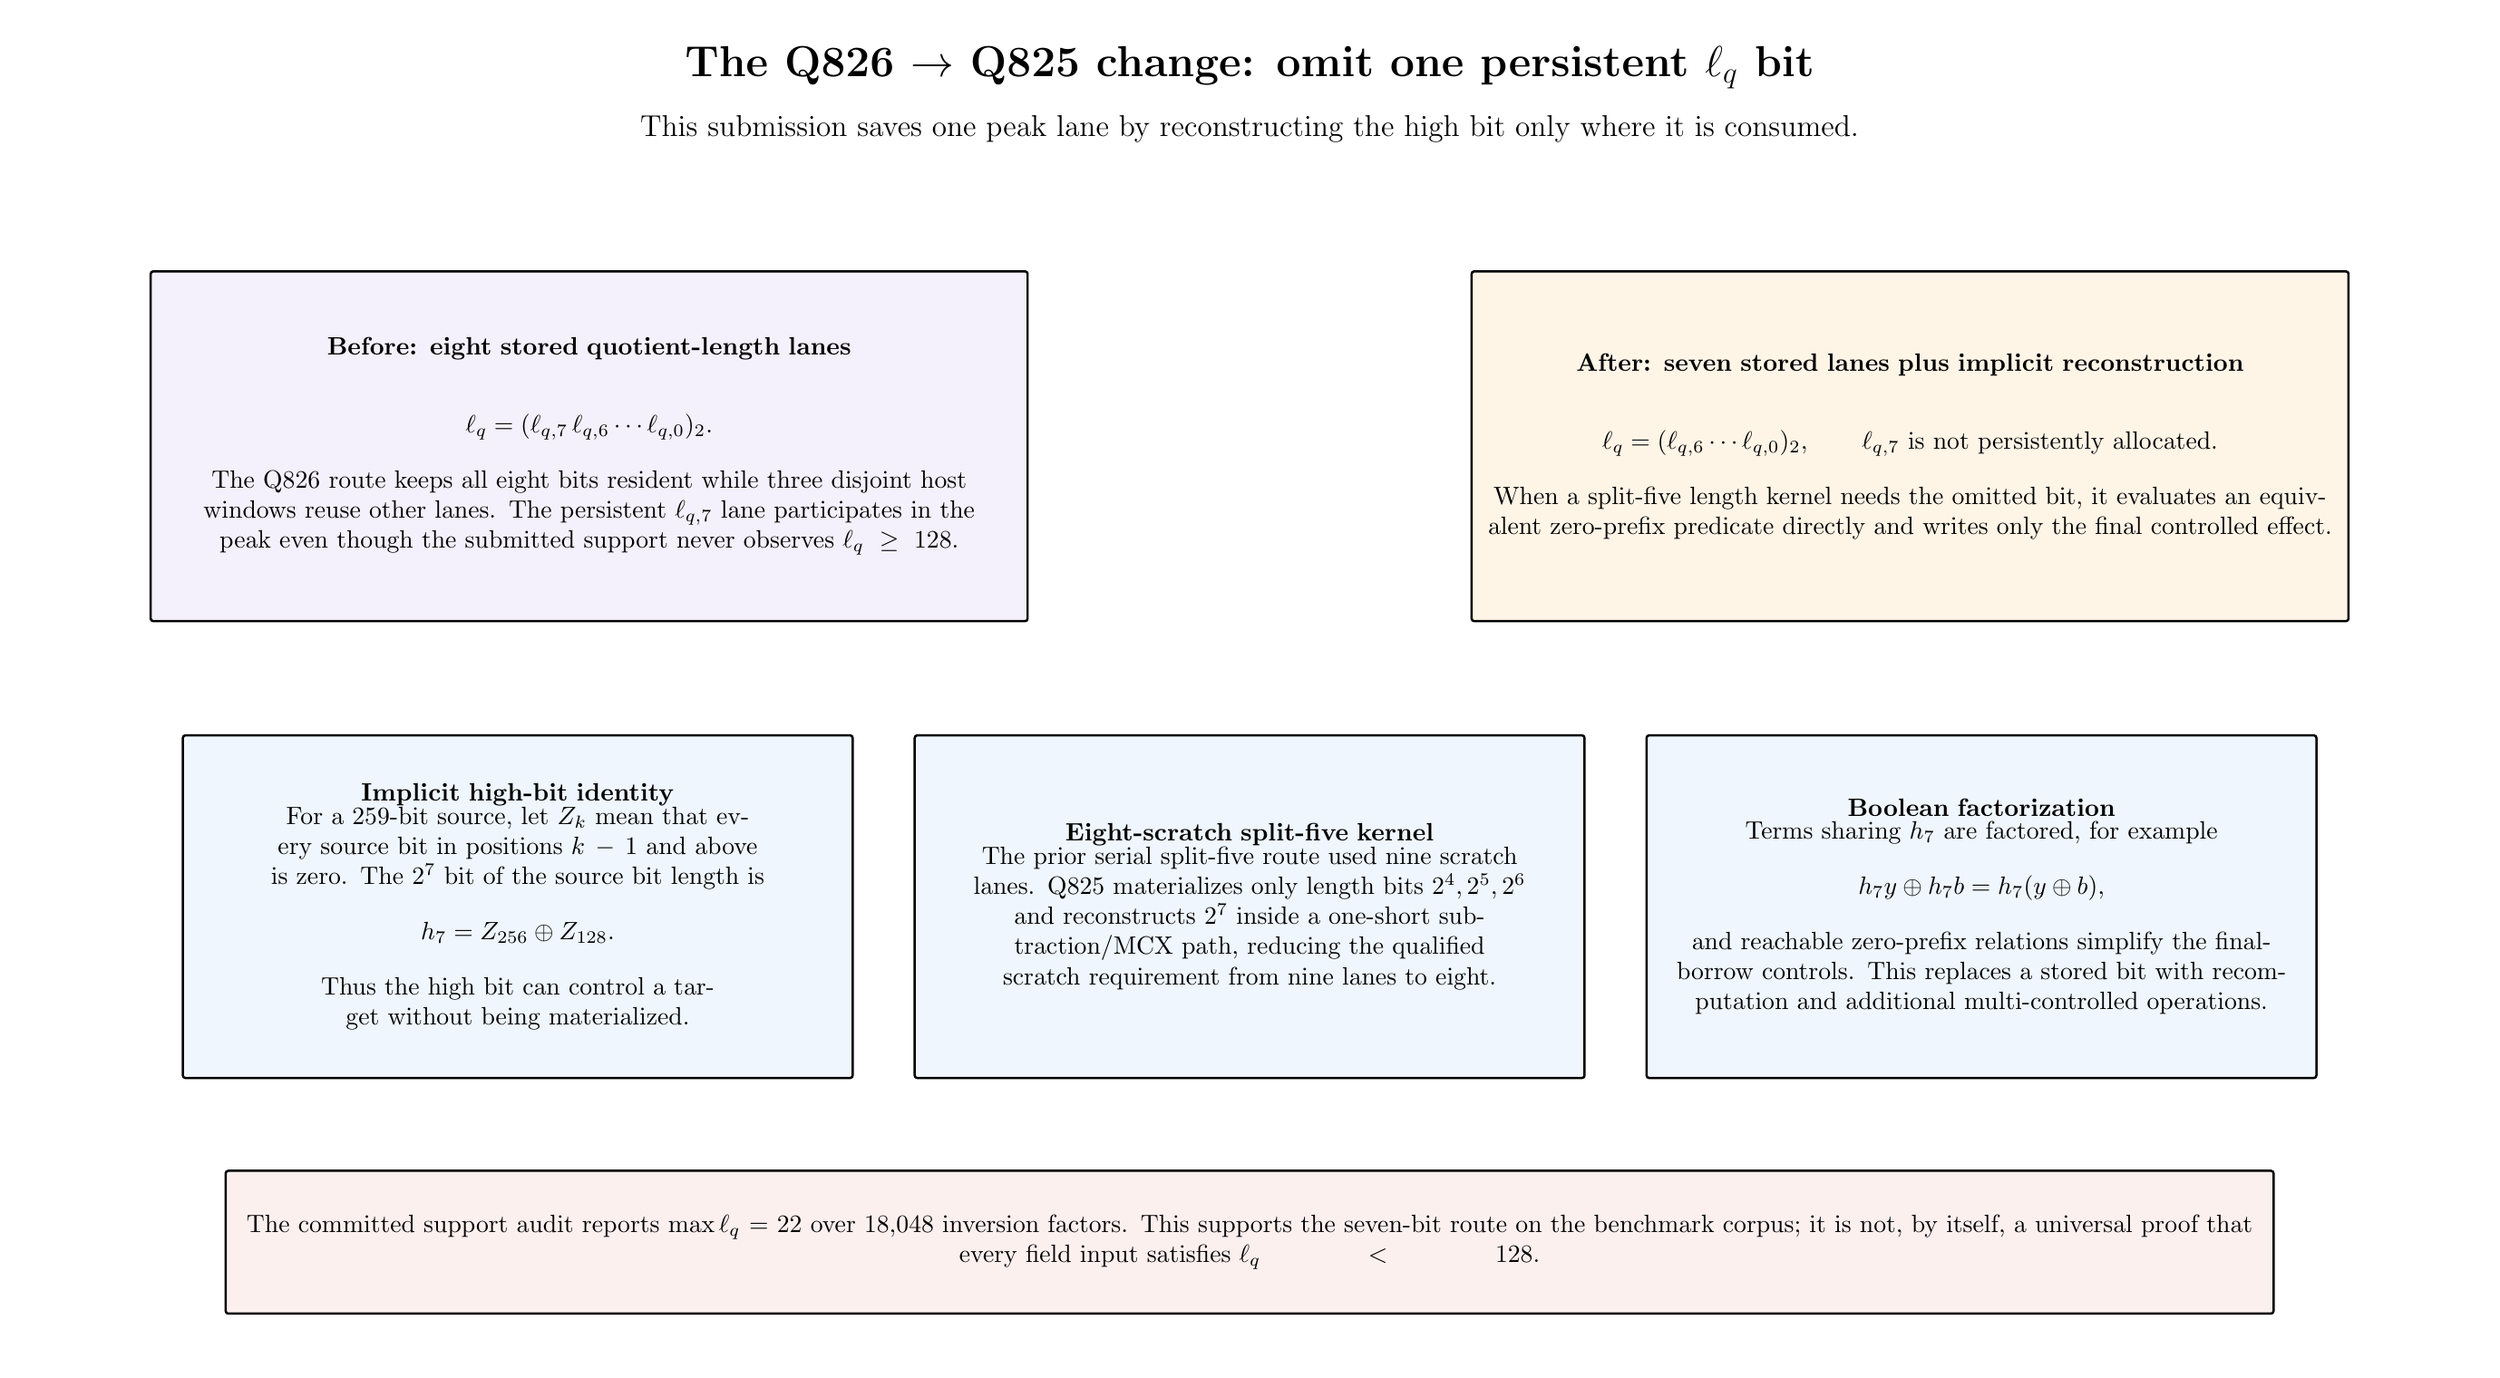
\begin{tikzpicture}[x=1cm,y=1cm]
  \path[use as bounding box] (0,0) rectangle (34.3,18.6);
  \node[font=\LARGE\bfseries] at (17.15,18.0)
    {The Q826 $\rightarrow$ Q825 change: omit one persistent $\ell_q$ bit};
  \node[font=\large] at (17.15,17.15)
    {This submission saves one peak lane by reconstructing the high bit only where it is consumed.};

  \node[inversion,text width=120mm,minimum height=49mm] at (7.9,12.7)
    {\textbf{Before: eight stored quotient-length lanes}\\[-1mm]
     \[
       \ell_q=(\ell_{q,7}\,\ell_{q,6}\cdots\ell_{q,0})_2.
     \]
     The Q826 route keeps all eight bits resident while three disjoint host windows reuse other lanes.
     The persistent $\ell_{q,7}$ lane participates in the peak even though the submitted support never
     observes $\ell_q\ge128$.};
  \node[classical,text width=120mm,minimum height=49mm] at (26.4,12.7)
    {\textbf{After: seven stored lanes plus implicit reconstruction}\\[-1mm]
     \[
       \ell_q=(\ell_{q,6}\cdots\ell_{q,0})_2,
       \qquad \ell_{q,7}\text{ is not persistently allocated.}
     \]
     When a split-five length kernel needs the omitted bit, it evaluates an equivalent zero-prefix
     predicate directly and writes only the final controlled effect.};

  \node[detail,text width=91mm,minimum height=48mm] at (6.9,6.25)
    {\textbf{Implicit high-bit identity}\\[-1mm]
     For a $259$-bit source, let $Z_k$ mean that every source bit in positions $k-1$ and above is zero.
     The $2^7$ bit of the source bit length is
     \[
       h_7=Z_{256}\oplus Z_{128}.
     \]
     Thus the high bit can control a target without being materialized.};
  \node[detail,text width=91mm,minimum height=48mm] at (17.15,6.25)
    {\textbf{Eight-scratch split-five kernel}\\[-1mm]
     The prior serial split-five route used nine scratch lanes. Q825 materializes only length bits
     $2^4,2^5,2^6$ and reconstructs $2^7$ inside a one-short subtraction/MCX path, reducing the
     qualified scratch requirement from nine lanes to eight.};
  \node[detail,text width=91mm,minimum height=48mm] at (27.4,6.25)
    {\textbf{Boolean factorization}\\[-1mm]
     Terms sharing $h_7$ are factored, for example
     \[
       h_7y\oplus h_7b=h_7(y\oplus b),
     \]
     and reachable zero-prefix relations simplify the final-borrow controls. This replaces a stored bit
     with recomputation and additional multi-controlled operations.};

  \node[warning,text width=284mm,minimum height=20mm] at (17.15,1.55)
    {The committed support audit reports $\max\ell_q=22$ over $18{,}048$ inversion factors. This supports
     the seven-bit route on the benchmark corpus; it is not, by itself, a universal proof that every field input satisfies $\ell_q<128$.};
\end{tikzpicture}
\newpage

% ============================================================================
% Additional analysis: consuming the omitted Q825 metadata bit
% ============================================================================
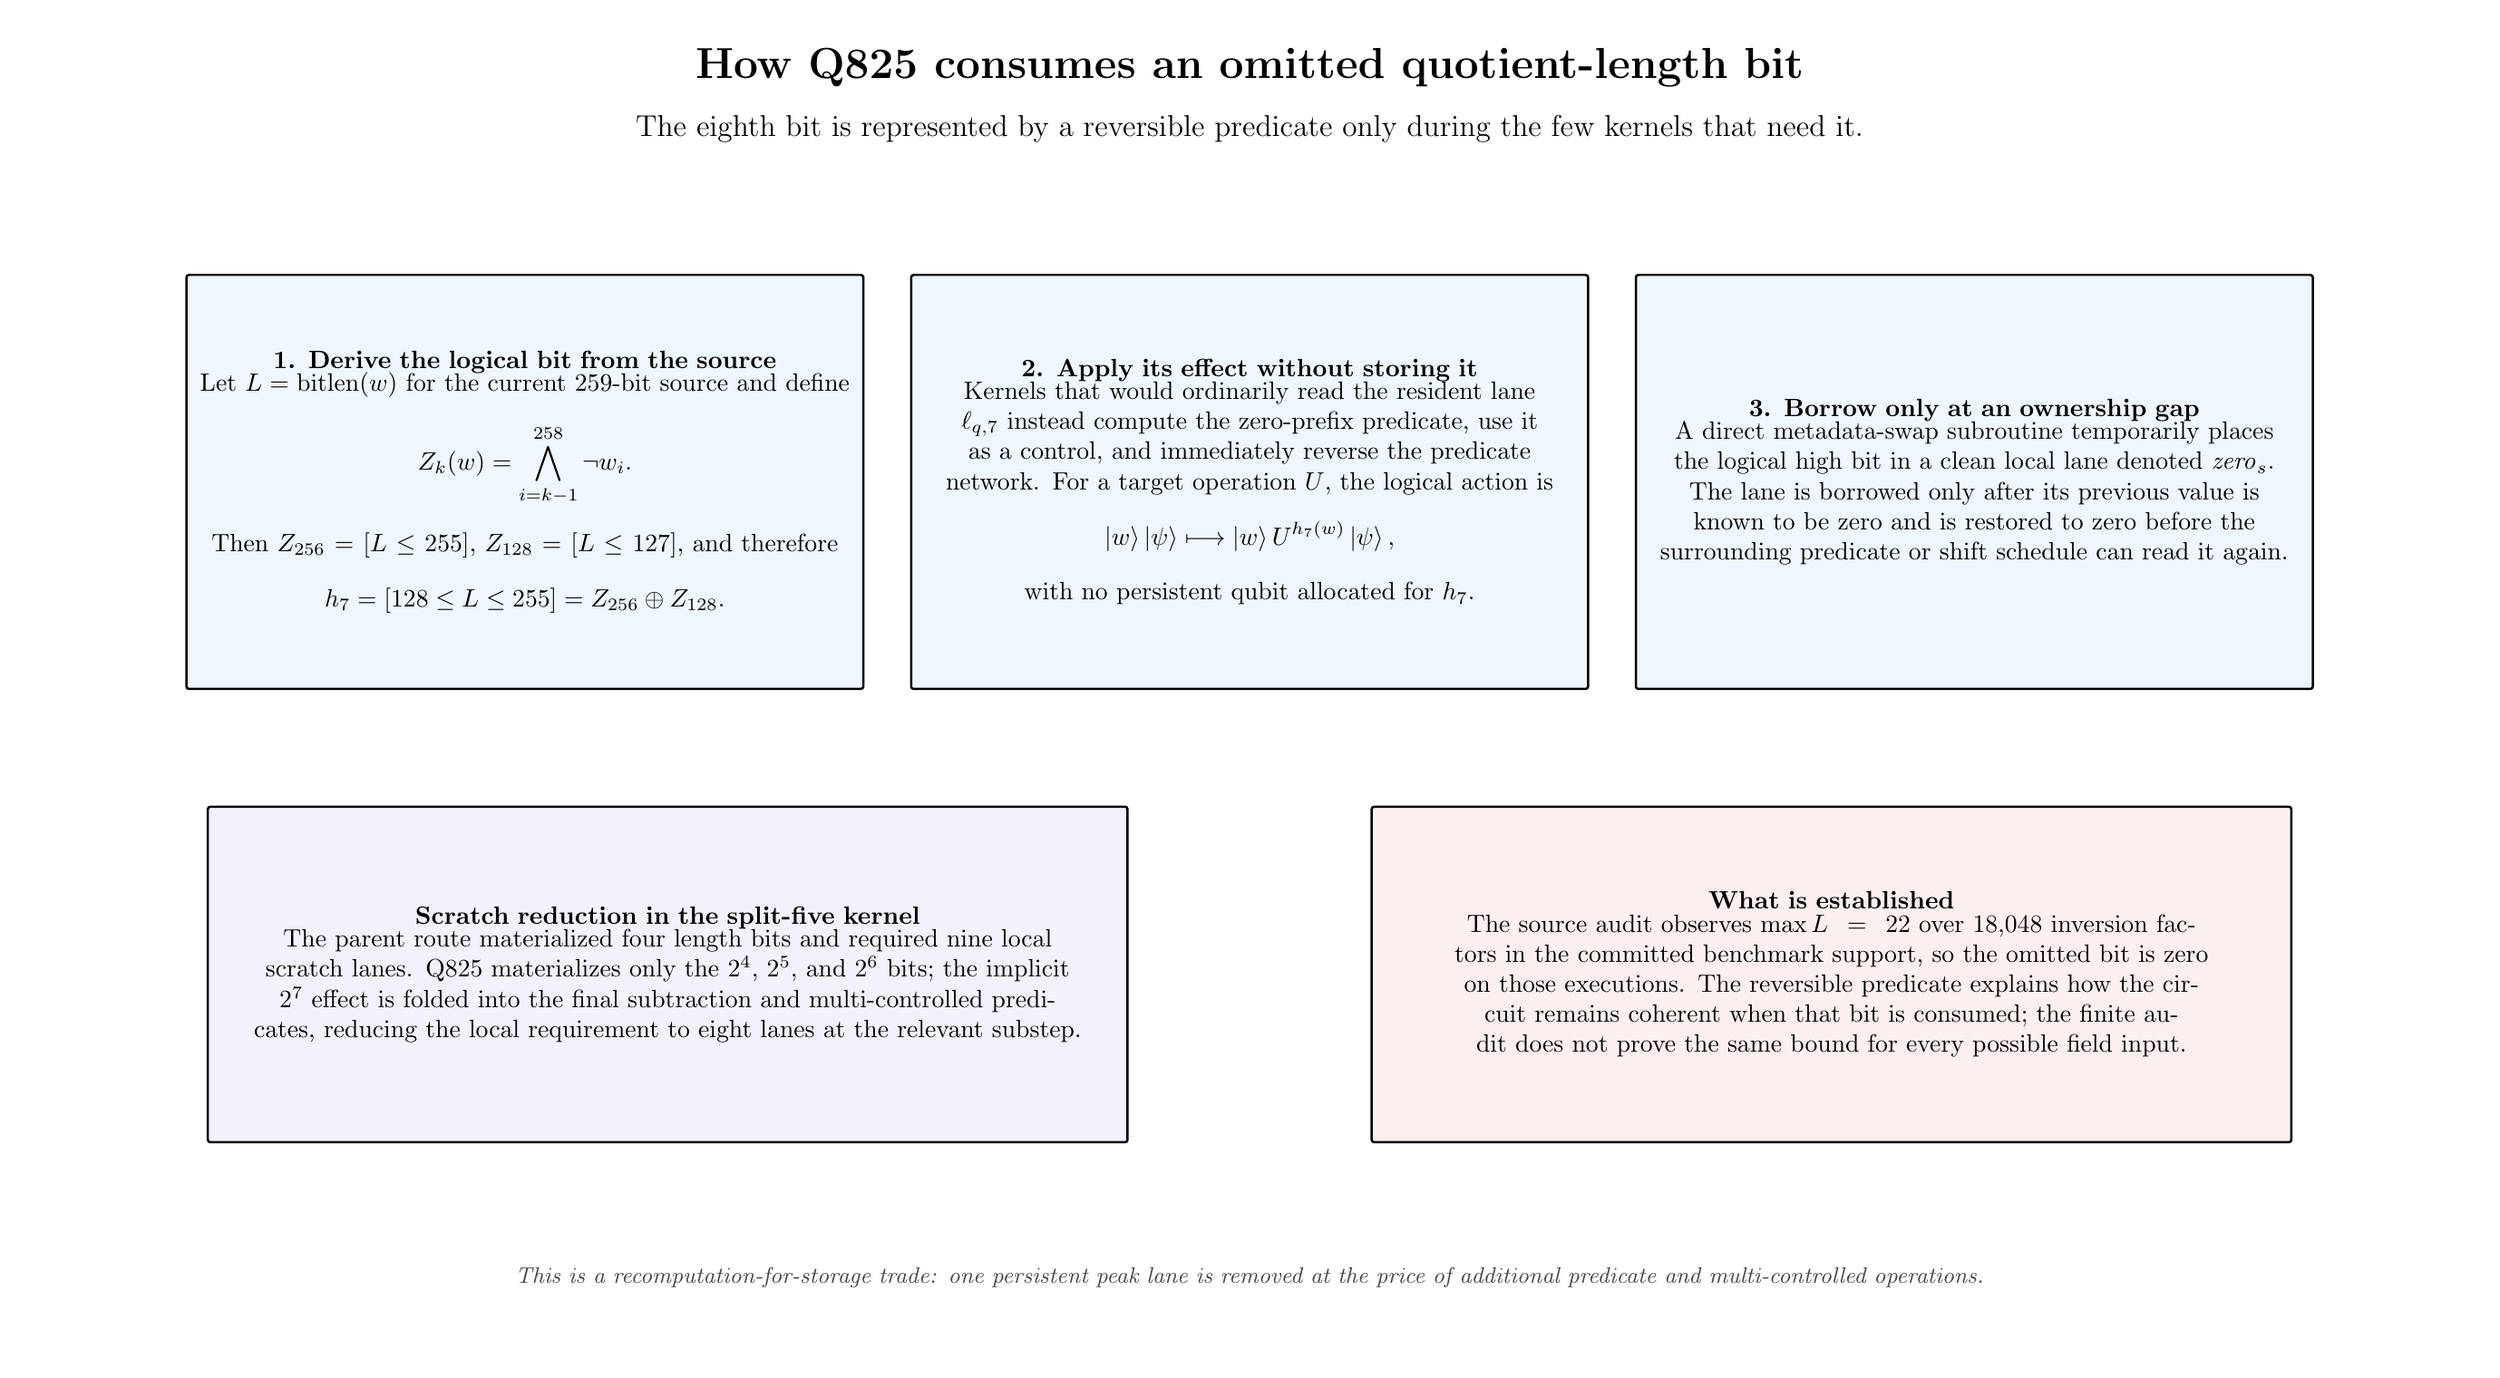
\begin{tikzpicture}[x=1cm,y=1cm]
  \path[use as bounding box] (0,0) rectangle (34.3,18.6);
  \node[font=\LARGE\bfseries] at (17.15,18.0)
    {How Q825 consumes an omitted quotient-length bit};
  \node[font=\large] at (17.15,17.15)
    {The eighth bit is represented by a reversible predicate only during the few kernels that need it.};

  \node[detail,text width=92mm,minimum height=58mm] at (7.0,12.2)
    {\textbf{1. Derive the logical bit from the source}\\[-1mm]
     Let $L=\operatorname{bitlen}(w)$ for the current $259$-bit source and define
     \[
       Z_k(w)=\bigwedge_{i=k-1}^{258}\neg w_i.
     \]
     Then $Z_{256}=[L\le255]$, $Z_{128}=[L\le127]$, and therefore
     \[
       h_7=[128\le L\le255]=Z_{256}\oplus Z_{128}.
     \]};
  \node[detail,text width=92mm,minimum height=58mm] at (17.15,12.2)
    {\textbf{2. Apply its effect without storing it}\\[-1mm]
     Kernels that would ordinarily read the resident lane $\ell_{q,7}$ instead compute the
     zero-prefix predicate, use it as a control, and immediately reverse the predicate network.
     For a target operation $U$, the logical action is
     \[
       \ket{w}\ket{\psi}\longmapsto
       \ket{w}U^{h_7(w)}\ket{\psi},
     \]
     with no persistent qubit allocated for $h_7$.};
  \node[detail,text width=92mm,minimum height=58mm] at (27.3,12.2)
    {\textbf{3. Borrow only at an ownership gap}\\[-1mm]
     A direct metadata-swap subroutine temporarily places the logical high bit in a clean local
     lane denoted $\mathit{zero}_s$. The lane is borrowed only after its previous value is known
     to be zero and is restored to zero before the surrounding predicate or shift schedule can
     read it again.};

  \node[inversion,text width=126mm,minimum height=47mm] at (9.0,5.3)
    {\textbf{Scratch reduction in the split-five kernel}\\[-1mm]
     The parent route materialized four length bits and required nine local scratch lanes. Q825
     materializes only the $2^4$, $2^5$, and $2^6$ bits; the implicit $2^7$ effect is folded into
     the final subtraction and multi-controlled predicates, reducing the local requirement to
     eight lanes at the relevant substep.};
  \node[warning,text width=126mm,minimum height=47mm] at (25.3,5.3)
    {\textbf{What is established}\\[-1mm]
     The source audit observes $\max L=22$ over $18{,}048$ inversion factors in the committed
     benchmark support, so the omitted bit is zero on those executions. The reversible predicate
     explains how the circuit remains coherent when that bit is consumed; the finite audit does
     not prove the same bound for every possible field input.};

  \node[note,text width=30cm,align=center,font=\small\itshape] at (17.15,1.05)
    {This is a recomputation-for-storage trade: one persistent peak lane is removed at the price of additional predicate and multi-controlled operations.};
\end{tikzpicture}
\newpage

% ============================================================================
% Page 10
% ============================================================================
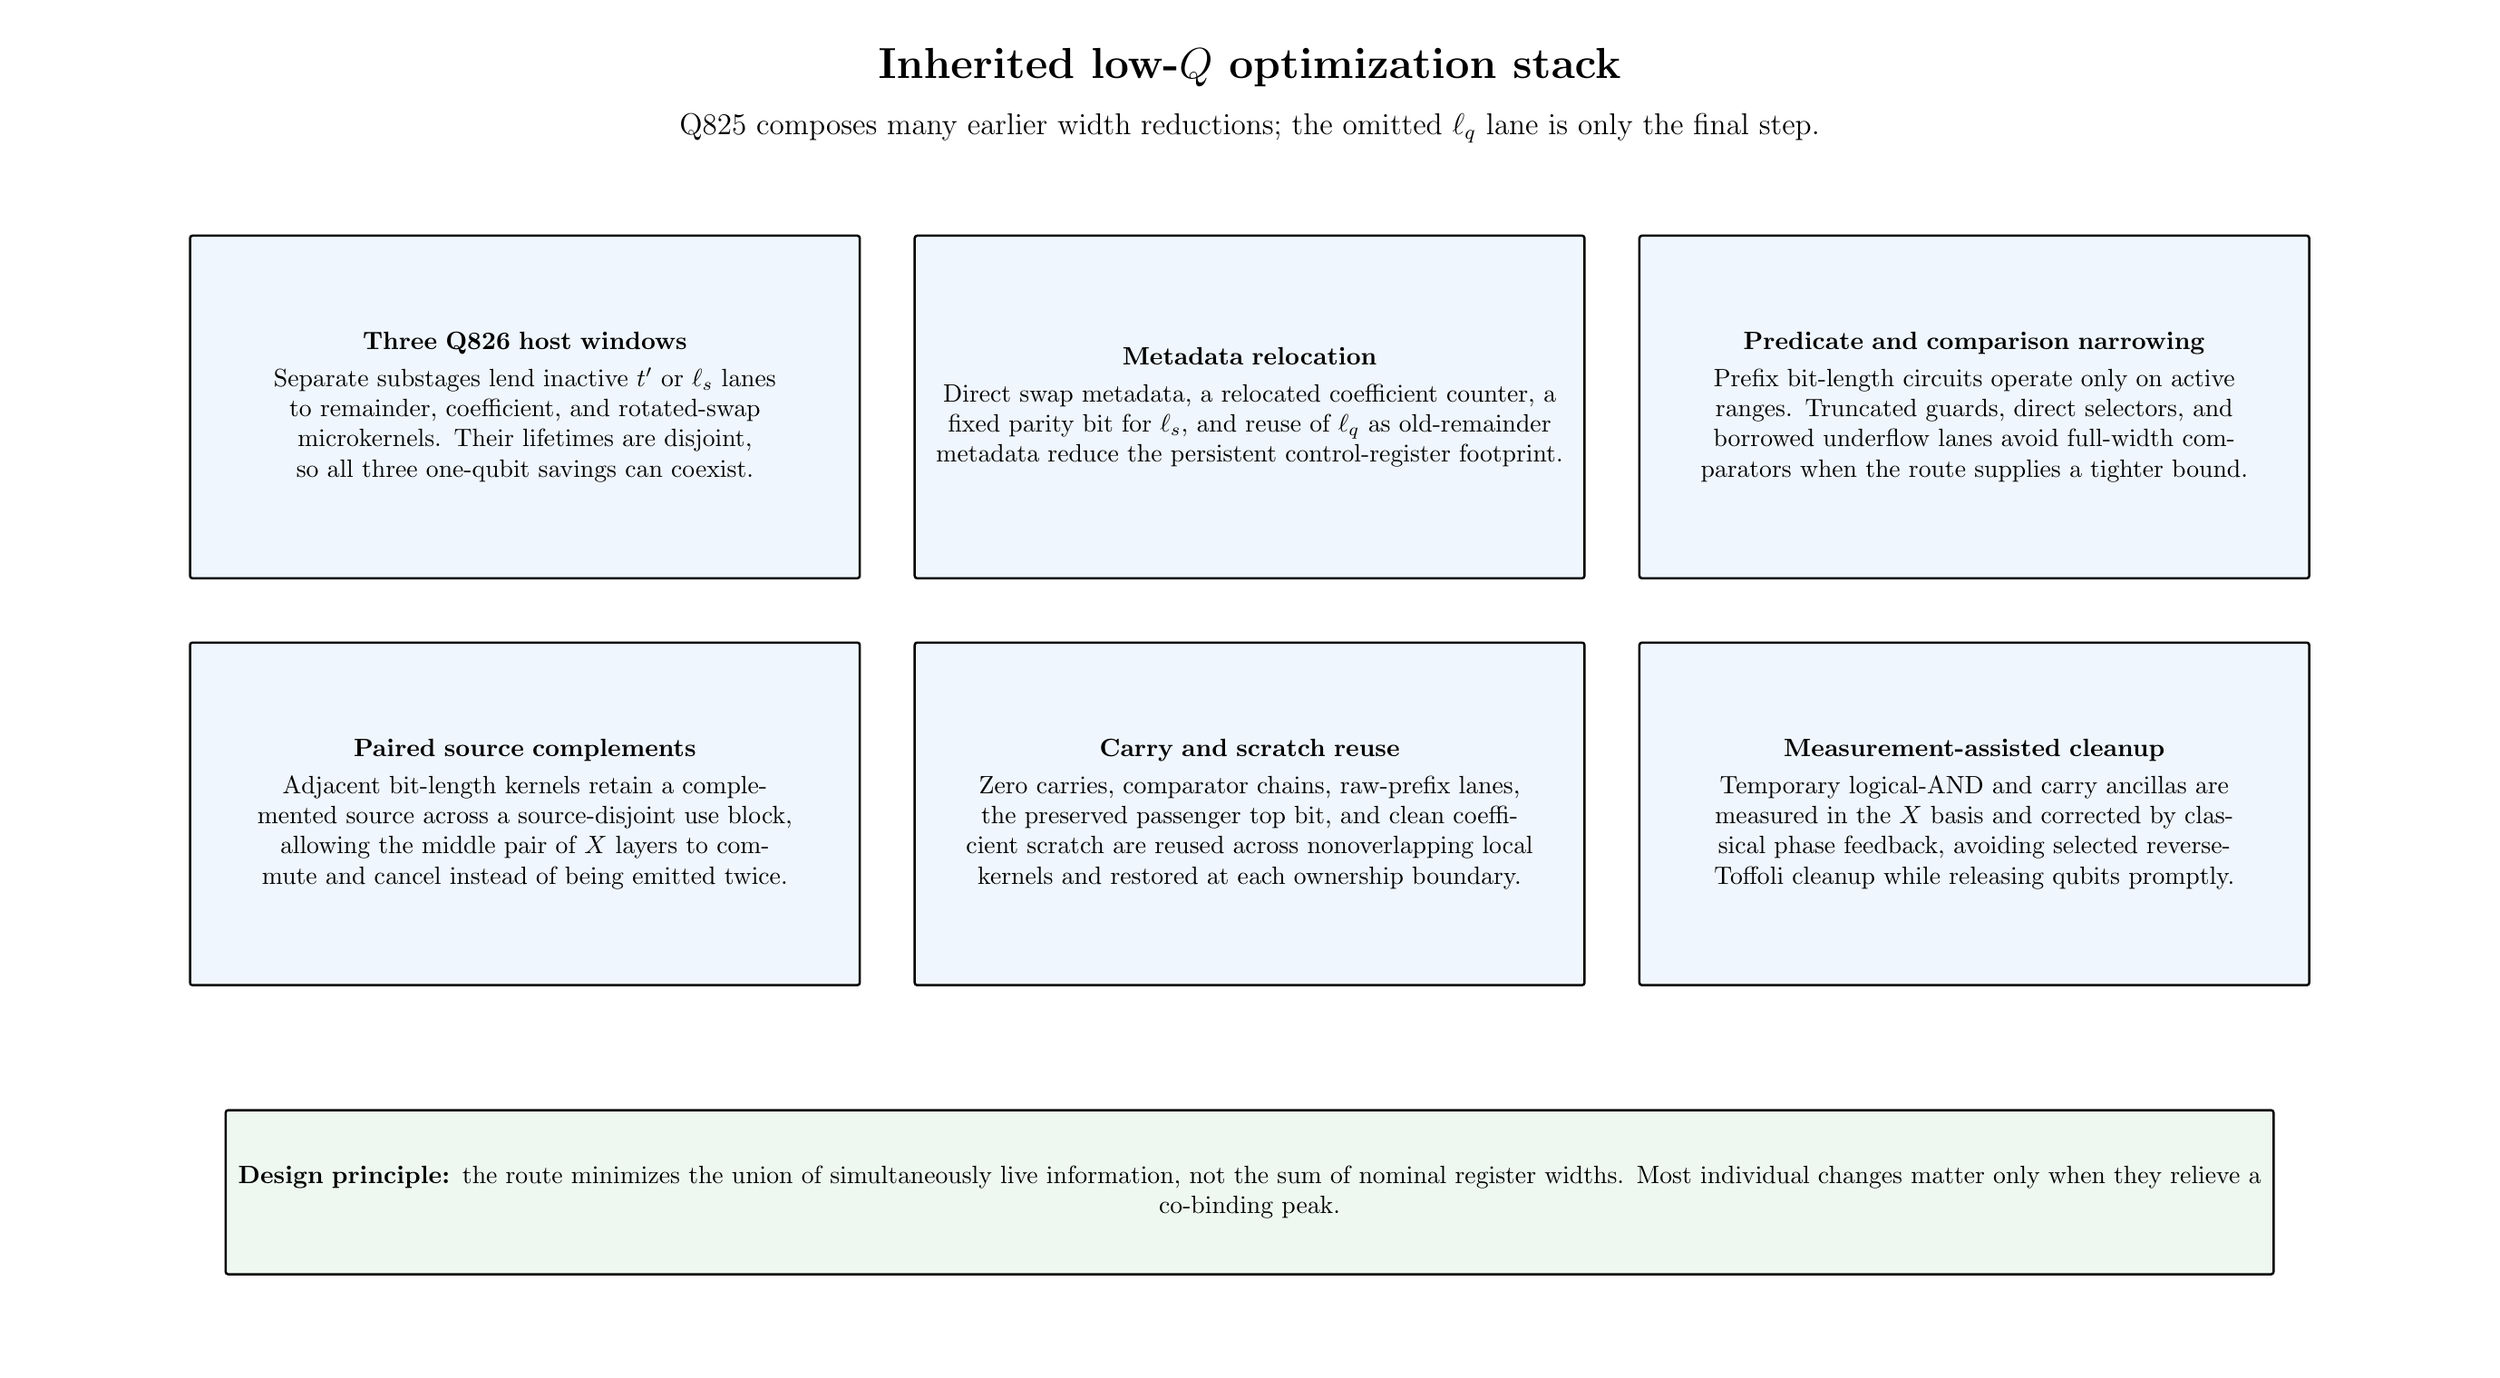
\begin{tikzpicture}[x=1cm,y=1cm]
  \path[use as bounding box] (0,0) rectangle (34.3,18.6);
  \node[font=\LARGE\bfseries] at (17.15,18.0)
    {Inherited low-$Q$ optimization stack};
  \node[font=\large] at (17.15,17.15)
    {Q825 composes many earlier width reductions; the omitted $\ell_q$ lane is only the final step.};

  \node[detail,text width=91mm,minimum height=48mm] at (7.0,13.25)
    {\textbf{Three Q826 host windows}\\[1mm]
     Separate substages lend inactive $t'$ or $\ell_s$ lanes to remainder, coefficient, and rotated-swap
     microkernels. Their lifetimes are disjoint, so all three one-qubit savings can coexist.};
  \node[detail,text width=91mm,minimum height=48mm] at (17.15,13.25)
    {\textbf{Metadata relocation}\\[1mm]
     Direct swap metadata, a relocated coefficient counter, a fixed parity bit for $\ell_s$, and reuse of
     $\ell_q$ as old-remainder metadata reduce the persistent control-register footprint.};
  \node[detail,text width=91mm,minimum height=48mm] at (27.3,13.25)
    {\textbf{Predicate and comparison narrowing}\\[1mm]
     Prefix bit-length circuits operate only on active ranges. Truncated guards, direct selectors, and
     borrowed underflow lanes avoid full-width comparators when the route supplies a tighter bound.};

  \node[detail,text width=91mm,minimum height=48mm] at (7.0,7.55)
    {\textbf{Paired source complements}\\[1mm]
     Adjacent bit-length kernels retain a complemented source across a source-disjoint use block, allowing
     the middle pair of $X$ layers to commute and cancel instead of being emitted twice.};
  \node[detail,text width=91mm,minimum height=48mm] at (17.15,7.55)
    {\textbf{Carry and scratch reuse}\\[1mm]
     Zero carries, comparator chains, raw-prefix lanes, the preserved passenger top bit, and clean coefficient
     scratch are reused across nonoverlapping local kernels and restored at each ownership boundary.};
  \node[detail,text width=91mm,minimum height=48mm] at (27.3,7.55)
    {\textbf{Measurement-assisted cleanup}\\[1mm]
     Temporary logical-AND and carry ancillas are measured in the $X$ basis and corrected by classical phase
     feedback, avoiding selected reverse-Toffoli cleanup while releasing qubits promptly.};

  \node[result,text width=284mm,minimum height=23mm] at (17.15,2.25)
    {\textbf{Design principle:} the route minimizes the union of simultaneously live information, not the sum
     of nominal register widths. Most individual changes matter only when they relieve a co-binding peak.};
\end{tikzpicture}
\newpage

% ============================================================================
% Page 11
% ============================================================================
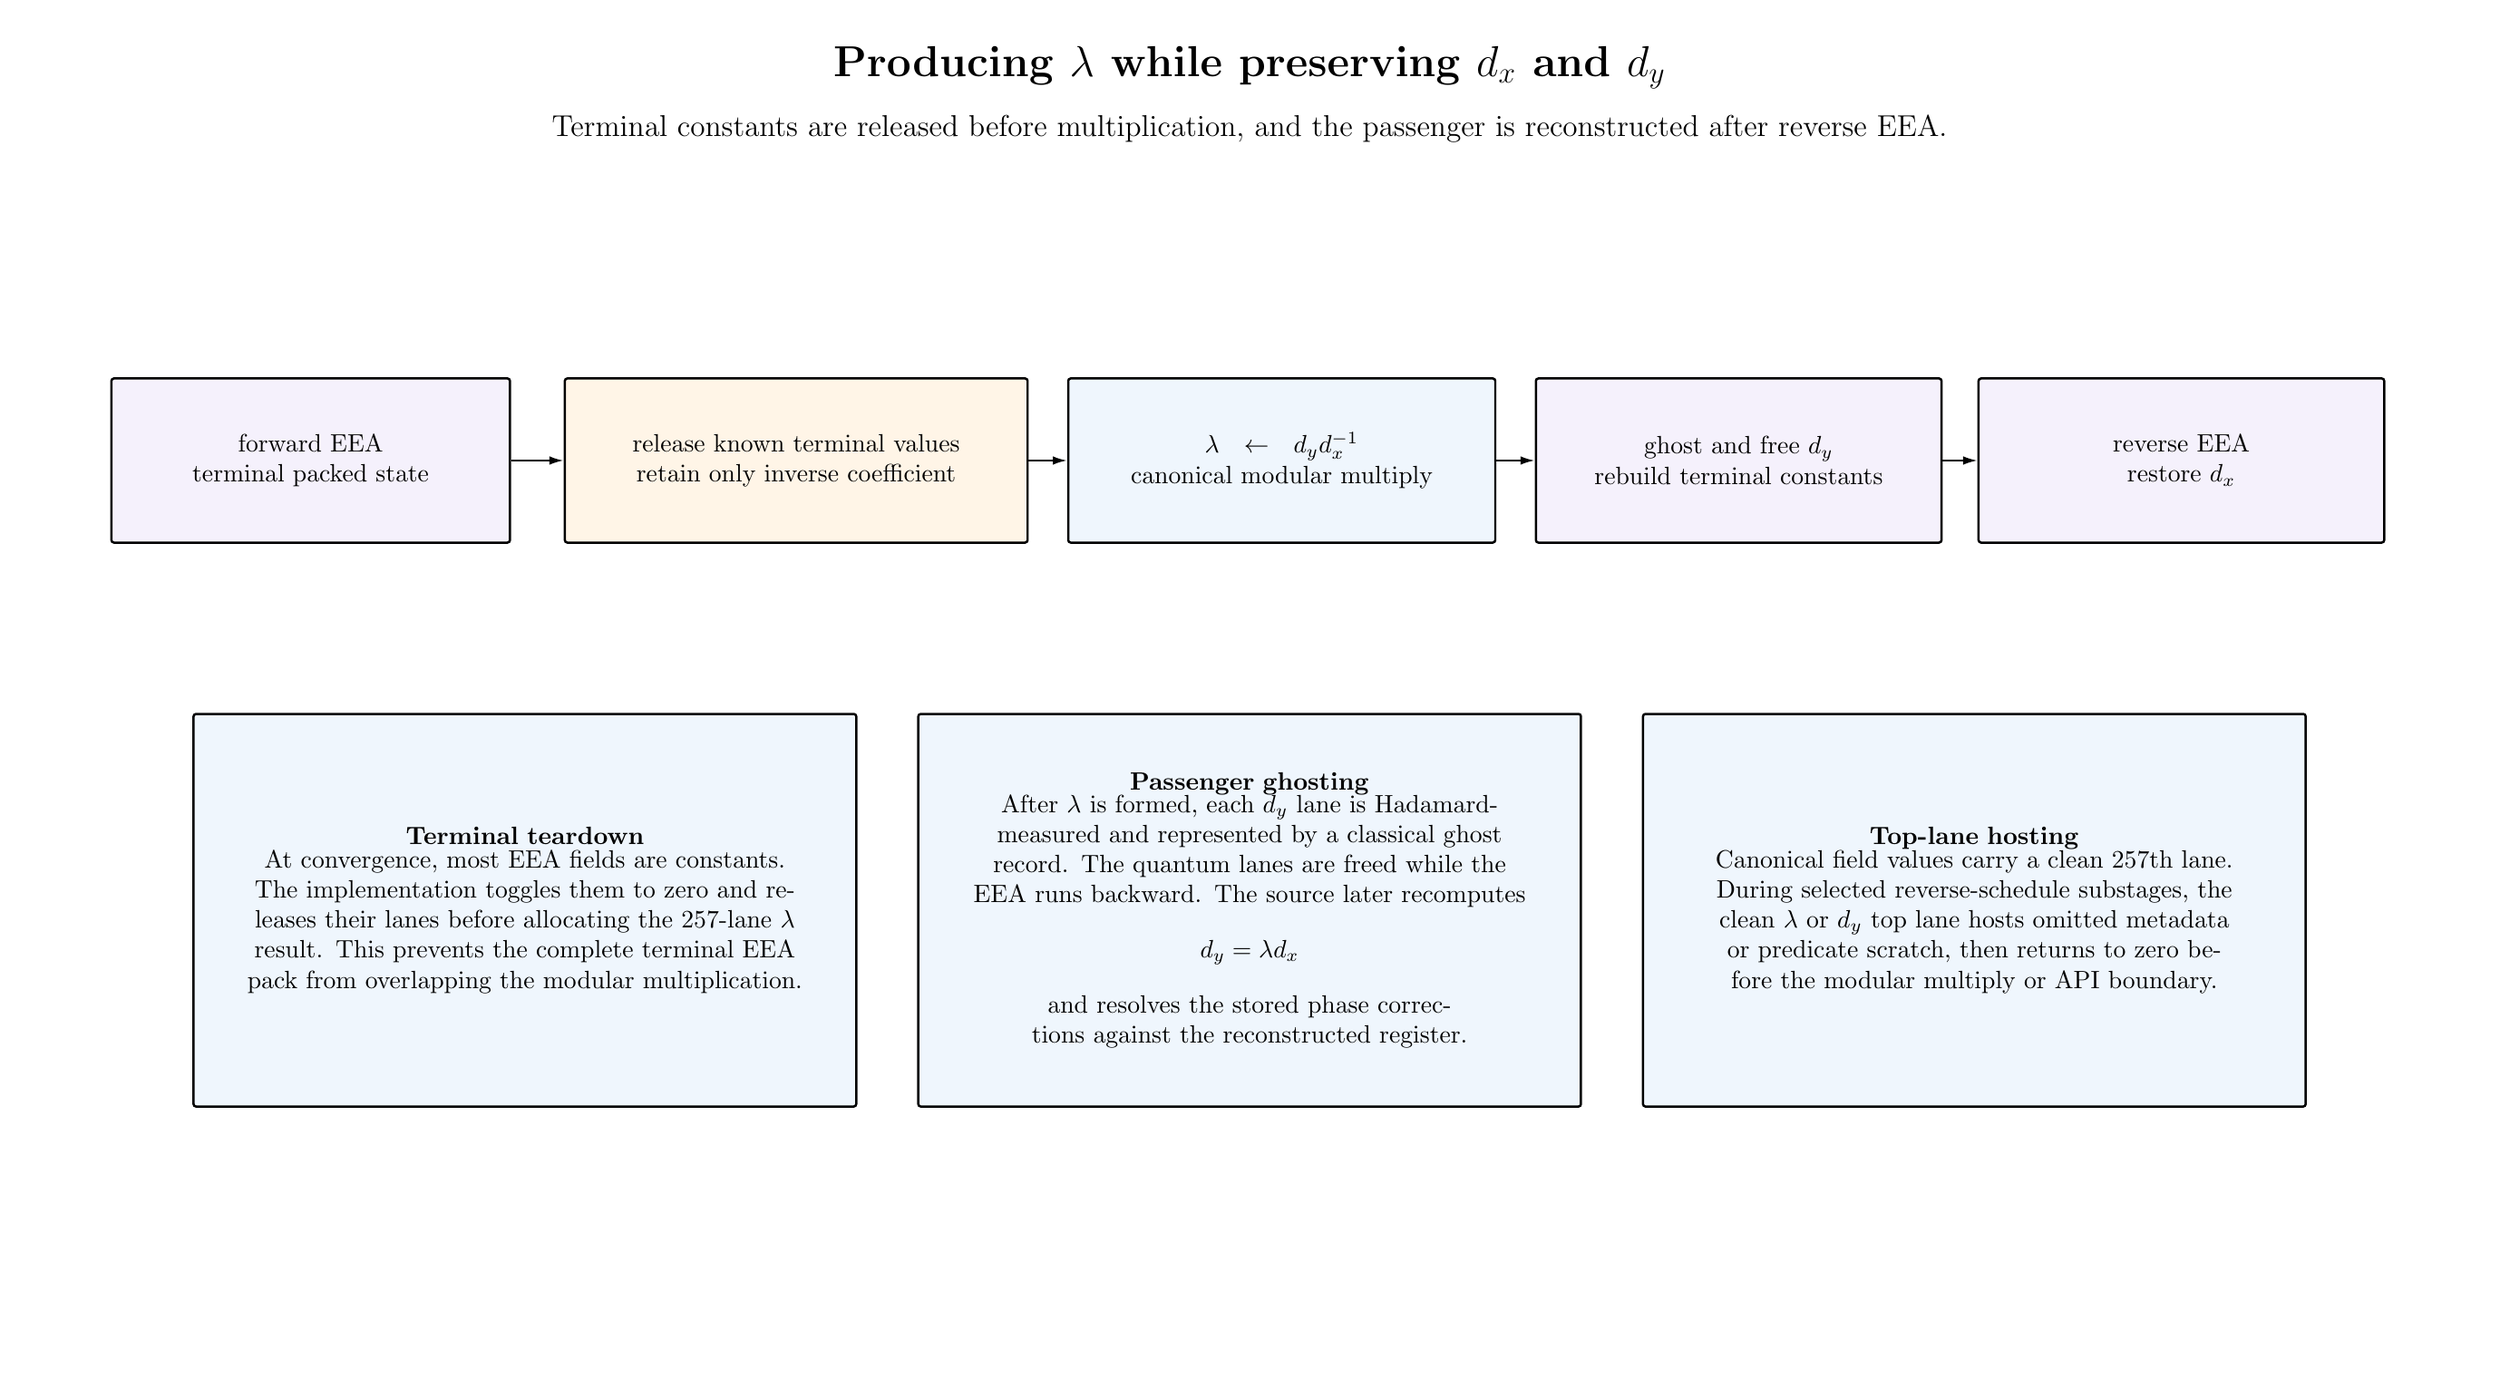
\begin{tikzpicture}[x=1cm,y=1cm]
  \path[use as bounding box] (0,0) rectangle (34.3,18.6);
  \node[font=\LARGE\bfseries] at (17.15,18.0)
    {Producing $\lambda$ while preserving $d_x$ and $d_y$};
  \node[font=\large] at (17.15,17.15)
    {Terminal constants are released before multiplication, and the passenger is reconstructed after reverse EEA.};

  \node[inversion,text width=53mm,minimum height=23mm] (A) at (4.0,12.5)
    {forward EEA\\terminal packed state};
  \node[classical,text width=62mm,minimum height=23mm] (B) at (10.8,12.5)
    {release known terminal values\\retain only inverse coefficient};
  \node[gate,text width=57mm,minimum height=23mm] (C) at (17.6,12.5)
    {$\lambda\gets d_y d_x^{-1}$\\canonical modular multiply};
  \node[inversion,text width=54mm,minimum height=23mm] (D) at (24.0,12.5)
    {ghost and free $d_y$\\rebuild terminal constants};
  \node[inversion,text width=54mm,minimum height=23mm] (E) at (30.2,12.5)
    {reverse EEA\\restore $d_x$};
  \draw[flow] (A.east)--(B.west);
  \draw[flow] (B.east)--(C.west);
  \draw[flow] (C.east)--(D.west);
  \draw[flow] (D.east)--(E.west);

  \node[detail,text width=90mm,minimum height=55mm] at (7.0,6.2)
    {\textbf{Terminal teardown}\\[-1mm]
     At convergence, most EEA fields are constants. The implementation toggles them to zero and releases their
     lanes before allocating the $257$-lane $\lambda$ result. This prevents the complete terminal EEA pack from
     overlapping the modular multiplication.};
  \node[detail,text width=90mm,minimum height=55mm] at (17.15,6.2)
    {\textbf{Passenger ghosting}\\[-1mm]
     After $\lambda$ is formed, each $d_y$ lane is Hadamard-measured and represented by a classical ghost record.
     The quantum lanes are freed while the EEA runs backward. The source later recomputes
     \[
       d_y=\lambda d_x
     \]
     and resolves the stored phase corrections against the reconstructed register.};
  \node[detail,text width=90mm,minimum height=55mm] at (27.3,6.2)
    {\textbf{Top-lane hosting}\\[-1mm]
     Canonical field values carry a clean $257$th lane. During selected reverse-schedule substages, the clean
     $\lambda$ or $d_y$ top lane hosts omitted metadata or predicate scratch, then returns to zero before the
     modular multiply or API boundary.};
\end{tikzpicture}
\newpage

% ============================================================================
% Additional analysis: exact measurement-based register release
% ============================================================================
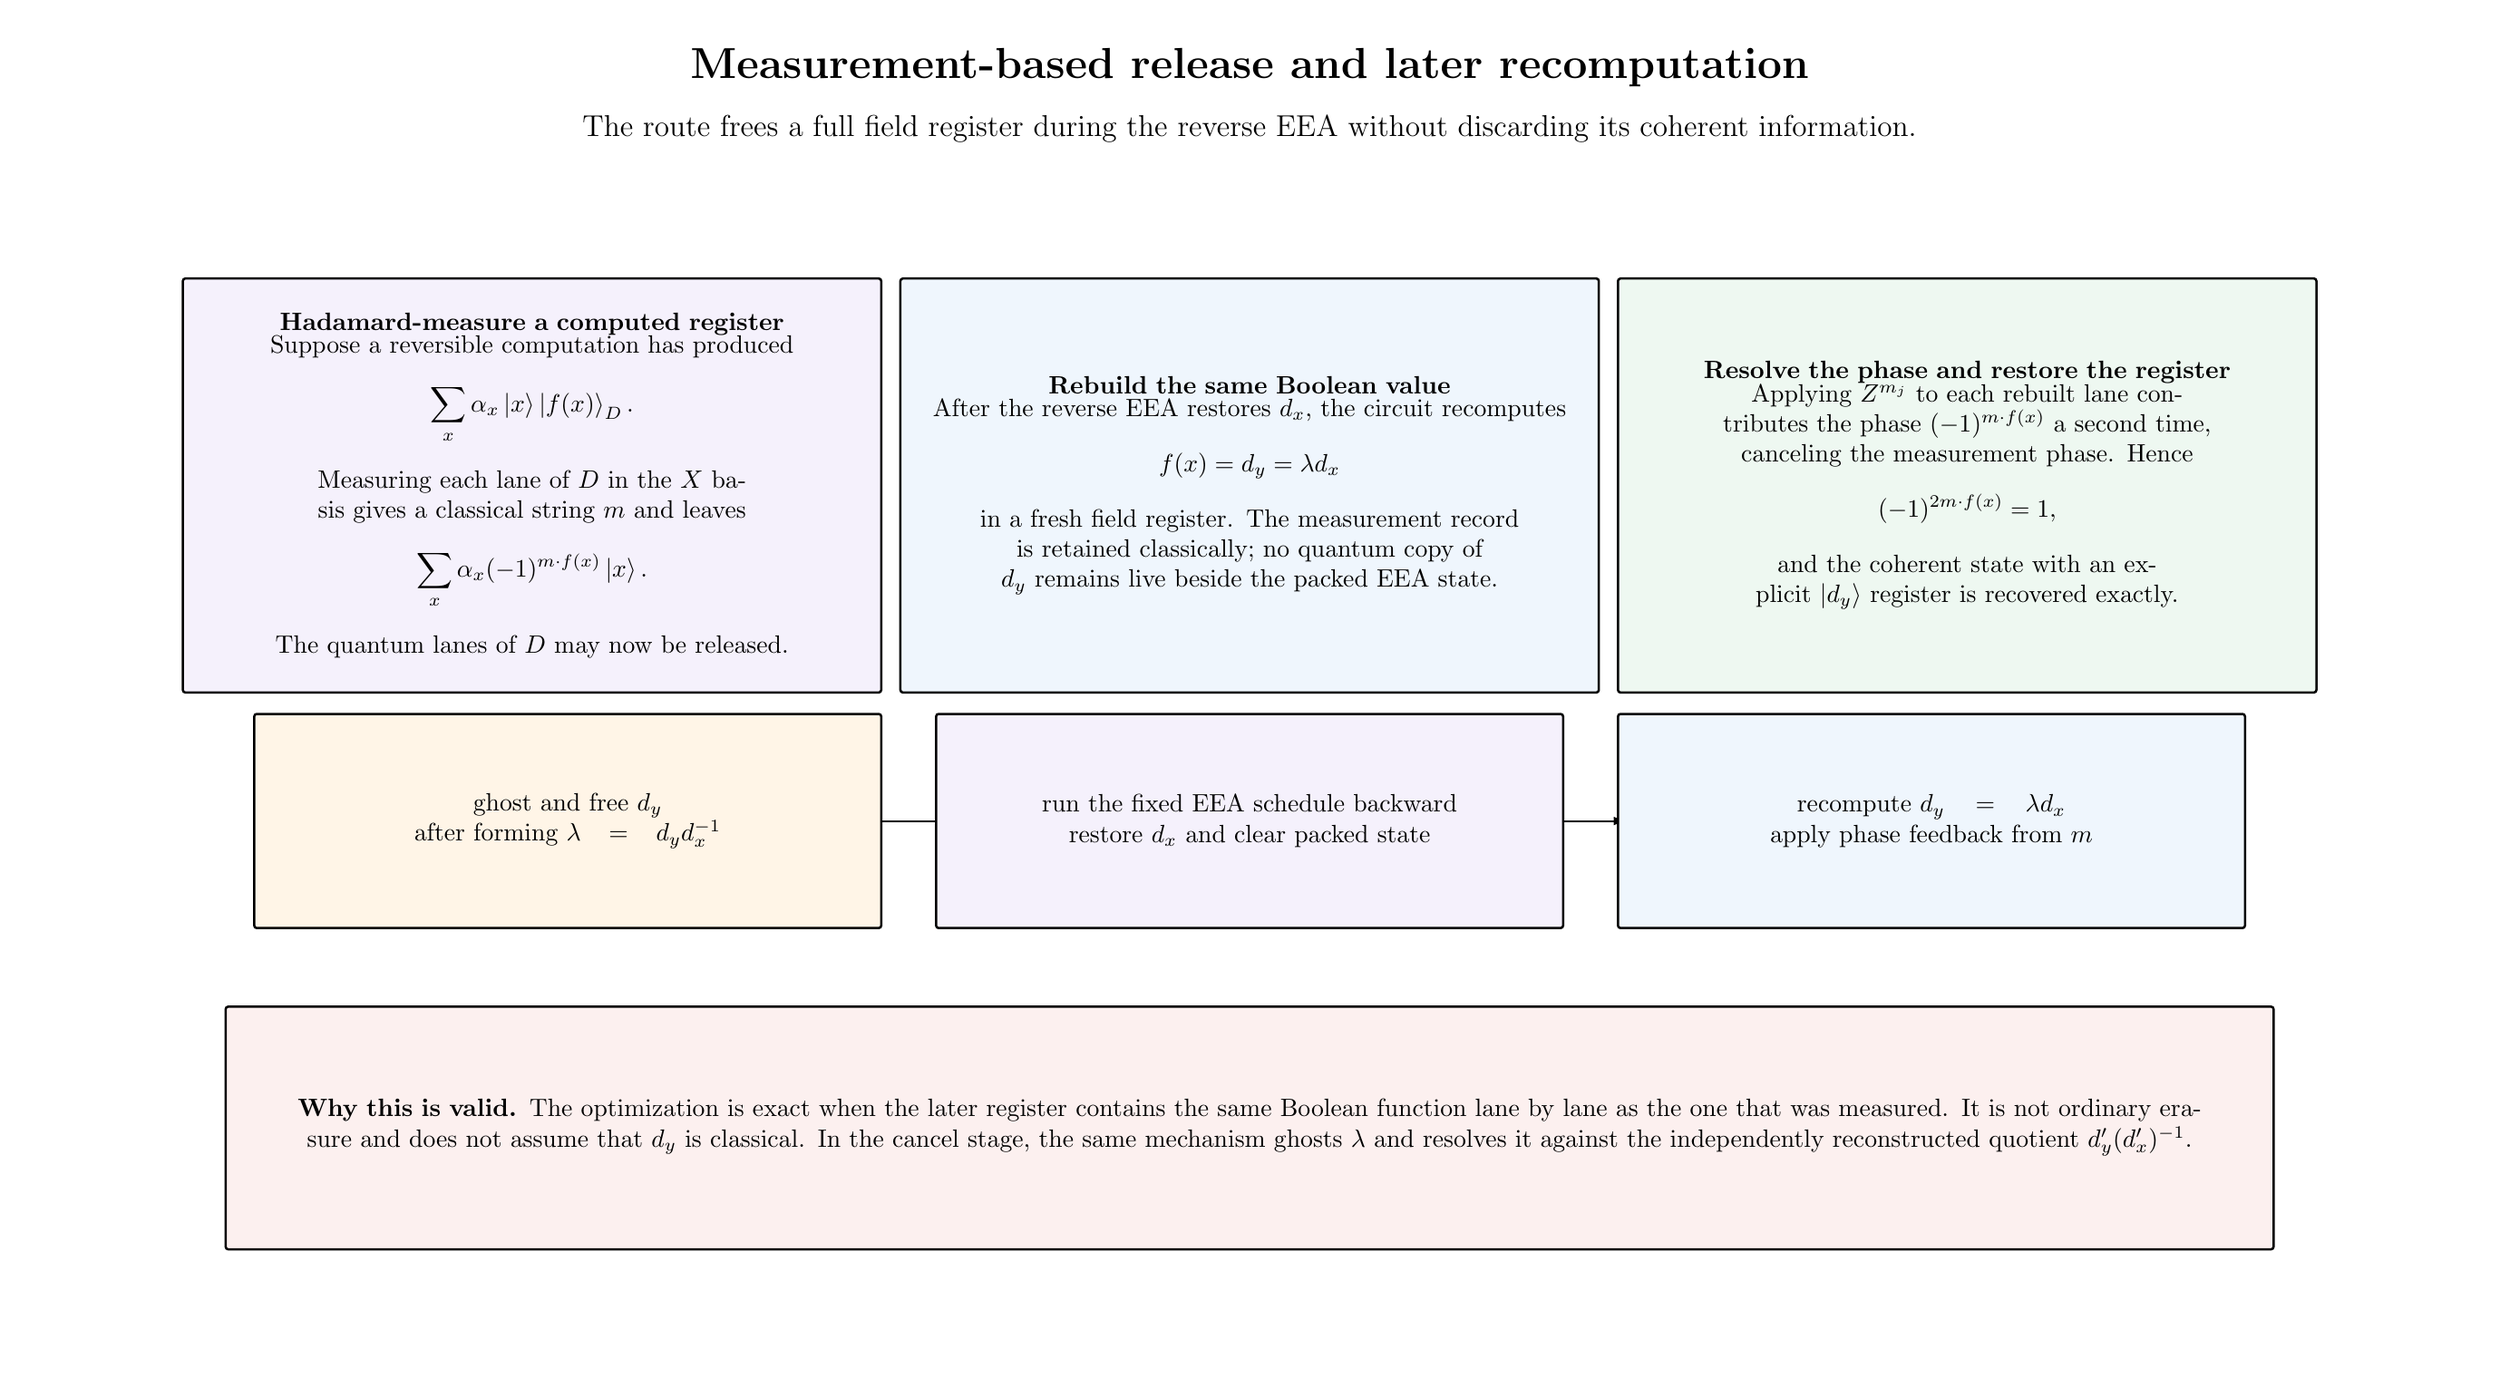
\begin{tikzpicture}[x=1cm,y=1cm]
  \path[use as bounding box] (0,0) rectangle (34.3,18.6);
  \node[font=\LARGE\bfseries] at (17.15,18.0)
    {Measurement-based release and later recomputation};
  \node[font=\large] at (17.15,17.15)
    {The route frees a full field register during the reverse EEA without discarding its coherent information.};

  \node[inversion,text width=95mm,minimum height=58mm] at (7.1,12.15)
    {\textbf{Hadamard-measure a computed register}\\[-1mm]
     Suppose a reversible computation has produced
     \[
       \sum_x \alpha_x\ket{x}\ket{f(x)}_D.
     \]
     Measuring each lane of $D$ in the $X$ basis gives a classical string $m$ and leaves
     \[
       \sum_x \alpha_x(-1)^{m\cdot f(x)}\ket{x}.
     \]
     The quantum lanes of $D$ may now be released.};
  \node[detail,text width=95mm,minimum height=58mm] at (17.15,12.15)
    {\textbf{Rebuild the same Boolean value}\\[-1mm]
     After the reverse EEA restores $d_x$, the circuit recomputes
     \[
       f(x)=d_y=\lambda d_x
     \]
     in a fresh field register. The measurement record is retained classically; no quantum copy
     of $d_y$ remains live beside the packed EEA state.};
  \node[result,text width=95mm,minimum height=58mm] at (27.2,12.15)
    {\textbf{Resolve the phase and restore the register}\\[-1mm]
     Applying $Z^{m_j}$ to each rebuilt lane contributes the phase
     $(-1)^{m\cdot f(x)}$ a second time, canceling the measurement phase. Hence
     \[
       (-1)^{2m\cdot f(x)}=1,
     \]
     and the coherent state with an explicit $\ket{d_y}$ register is recovered exactly.};

  \draw[flow] (11.85,7.45)--(14.0,7.45);
  \draw[flow] (20.3,7.45)--(22.45,7.45);
  \node[classical,text width=85mm,minimum height=30mm] at (7.6,7.45)
    {ghost and free $d_y$\\after forming $\lambda=d_y d_x^{-1}$};
  \node[inversion,text width=85mm,minimum height=30mm] at (17.15,7.45)
    {run the fixed EEA schedule backward\\restore $d_x$ and clear packed state};
  \node[gate,text width=85mm,minimum height=30mm] at (26.7,7.45)
    {recompute $d_y=\lambda d_x$\\apply phase feedback from $m$};

  \node[warning,text width=284mm,minimum height=34mm] at (17.15,3.15)
    {\textbf{Why this is valid.} The optimization is exact when the later register contains the same
     Boolean function lane by lane as the one that was measured. It is not ordinary erasure and does
     not assume that $d_y$ is classical. In the cancel stage, the same mechanism ghosts $\lambda$ and
     resolves it against the independently reconstructed quotient $d'_y(d'_x)^{-1}$.};
\end{tikzpicture}
\newpage

% ============================================================================
% Page 12
% ============================================================================
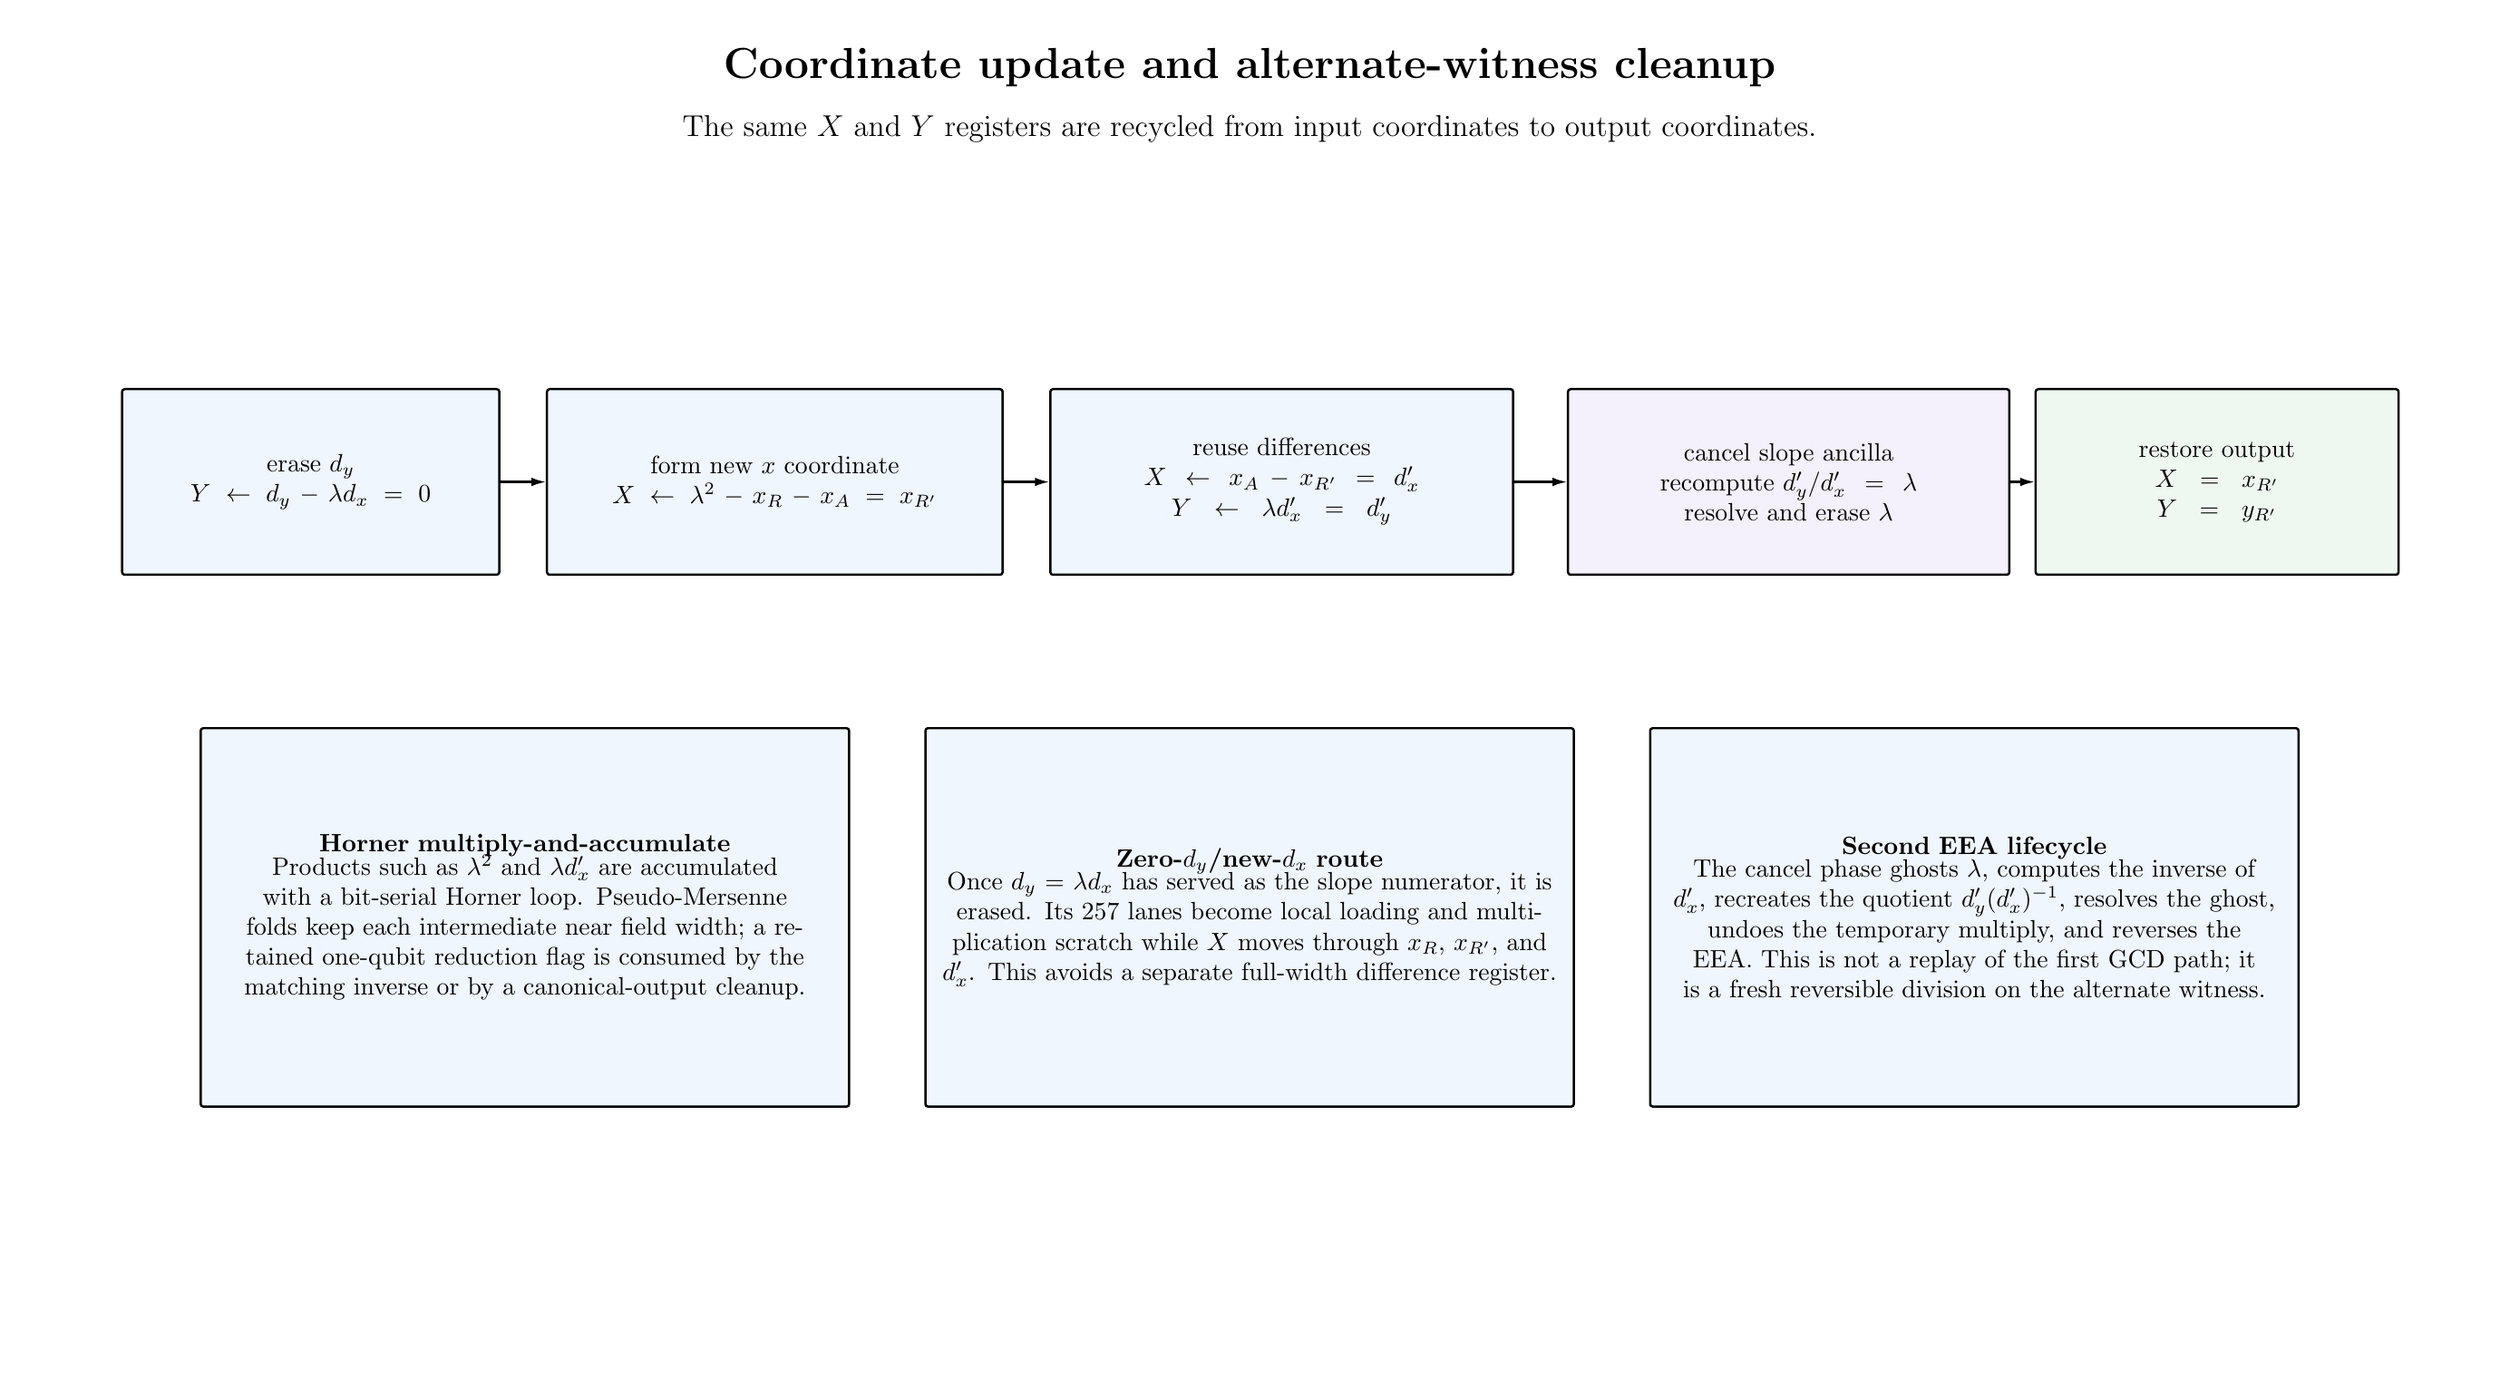
\begin{tikzpicture}[x=1cm,y=1cm]
  \path[use as bounding box] (0,0) rectangle (34.3,18.6);
  \node[font=\LARGE\bfseries] at (17.15,18.0)
    {Coordinate update and alternate-witness cleanup};
  \node[font=\large] at (17.15,17.15)
    {The same $X$ and $Y$ registers are recycled from input coordinates to output coordinates.};

  \node[gate,text width=50mm,minimum height=26mm] (Z) at (4.0,12.2)
    {erase $d_y$\\$Y\gets d_y-\lambda d_x=0$};
  \node[gate,text width=61mm,minimum height=26mm] (NX) at (10.5,12.2)
    {form new $x$ coordinate\\$X\gets\lambda^2-x_R-x_A=x_{R'}$};
  \node[gate,text width=62mm,minimum height=26mm] (ND) at (17.6,12.2)
    {reuse differences\\$X\gets x_A-x_{R'}=d'_x$\\$Y\gets\lambda d'_x=d'_y$};
  \node[inversion,text width=59mm,minimum height=26mm] (CAN) at (24.7,12.2)
    {cancel slope ancilla\\recompute $d'_y/d'_x=\lambda$\\resolve and erase $\lambda$};
  \node[result,text width=48mm,minimum height=26mm] (OUT) at (30.7,12.2)
    {restore output\\$X=x_{R'}$\\$Y=y_{R'}$};
  \draw[flow] (Z.east)--(NX.west);
  \draw[flow] (NX.east)--(ND.west);
  \draw[flow] (ND.east)--(CAN.west);
  \draw[flow] (CAN.east)--(OUT.west);

  \node[detail,text width=88mm,minimum height=53mm] at (7.0,6.1)
    {\textbf{Horner multiply-and-accumulate}\\[-1mm]
     Products such as $\lambda^2$ and $\lambda d'_x$ are accumulated with a bit-serial Horner loop.
     Pseudo-Mersenne folds keep each intermediate near field width; a retained one-qubit reduction flag is
     consumed by the matching inverse or by a canonical-output cleanup.};
  \node[detail,text width=88mm,minimum height=53mm] at (17.15,6.1)
    {\textbf{Zero-$d_y$/new-$d_x$ route}\\[-1mm]
     Once $d_y=\lambda d_x$ has served as the slope numerator, it is erased. Its $257$ lanes become local
     loading and multiplication scratch while $X$ moves through $x_R$, $x_{R'}$, and $d'_x$. This avoids a
     separate full-width difference register.};
  \node[detail,text width=88mm,minimum height=53mm] at (27.3,6.1)
    {\textbf{Second EEA lifecycle}\\[-1mm]
     The cancel phase ghosts $\lambda$, computes the inverse of $d'_x$, recreates the quotient
     $d'_y(d'_x)^{-1}$, resolves the ghost, undoes the temporary multiply, and reverses the EEA. This is not a
     replay of the first GCD path; it is a fresh reversible division on the alternate witness.};
\end{tikzpicture}
\newpage

% ============================================================================
% Additional analysis: fresh alternate-witness EEA lifecycle
% ============================================================================
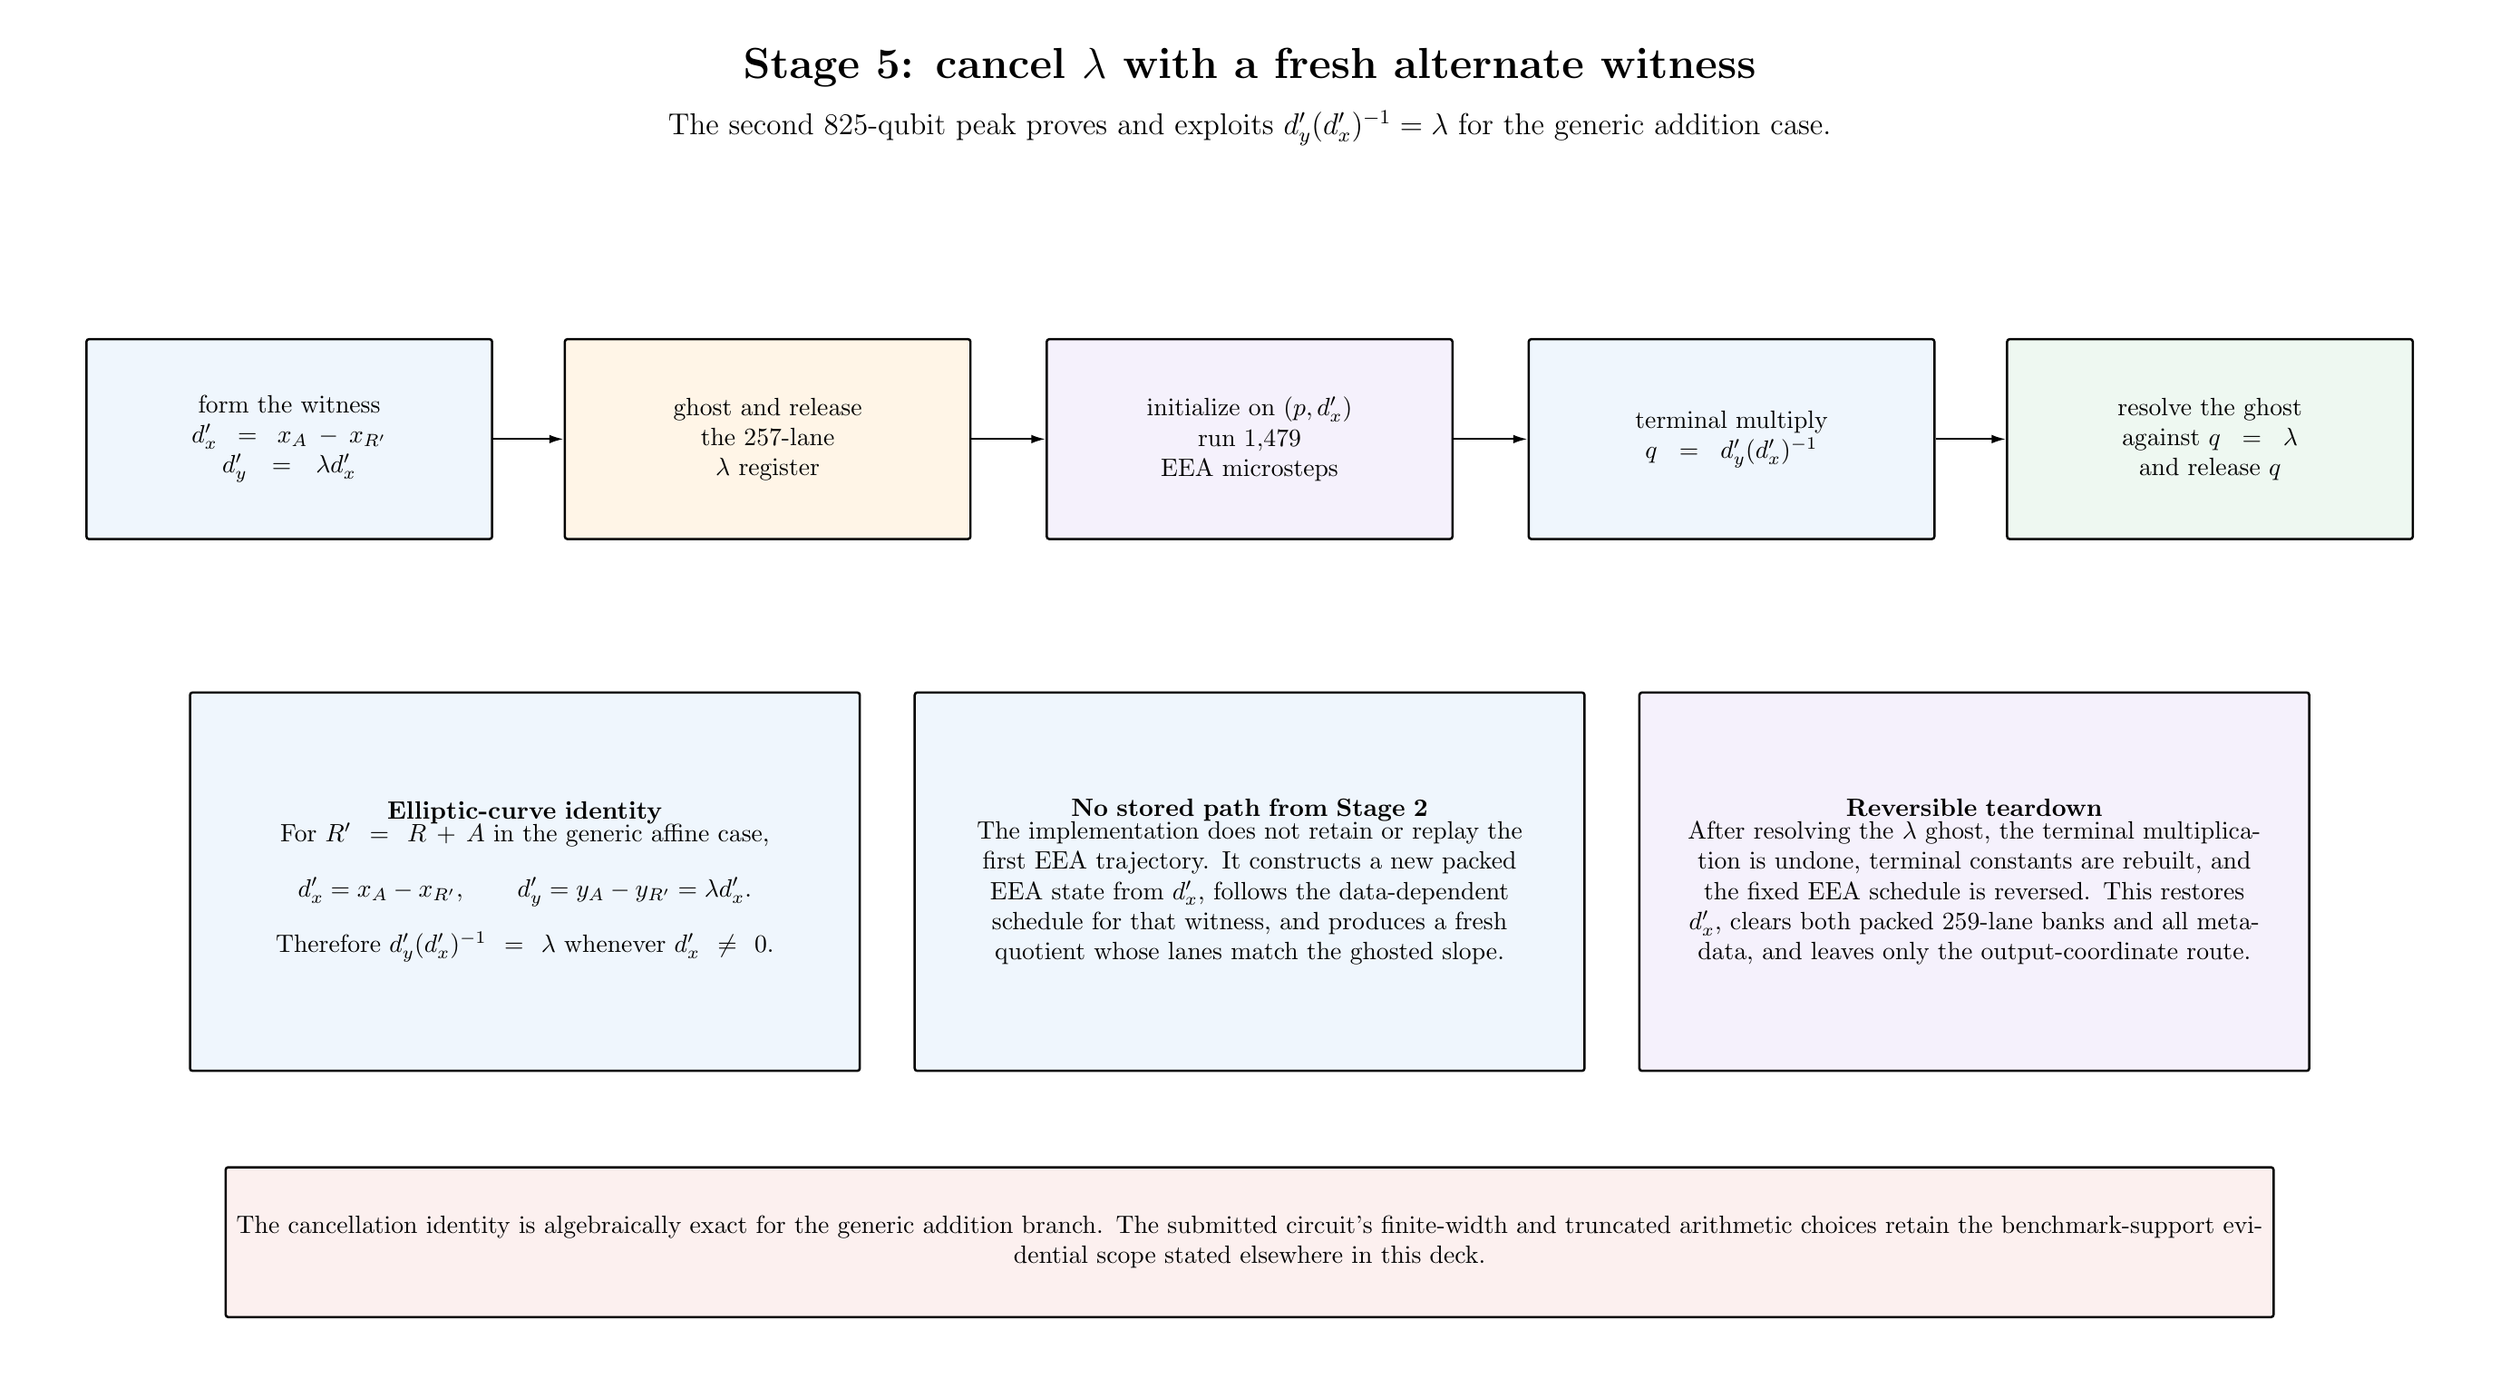
\begin{tikzpicture}[x=1cm,y=1cm]
  \path[use as bounding box] (0,0) rectangle (34.3,18.6);
  \node[font=\LARGE\bfseries] at (17.15,18.0)
    {Stage 5: cancel $\lambda$ with a fresh alternate witness};
  \node[font=\large] at (17.15,17.15)
    {The second 825-qubit peak proves and exploits $d'_y(d'_x)^{-1}=\lambda$ for the generic addition case.};

  \node[gate,text width=54mm,minimum height=28mm] (A1) at (3.7,12.8)
    {form the witness\\$d'_x=x_A-x_{R'}$\\$d'_y=\lambda d'_x$};
  \node[classical,text width=54mm,minimum height=28mm] (A2) at (10.4,12.8)
    {ghost and release\\the $257$-lane\\$\lambda$ register};
  \node[inversion,text width=54mm,minimum height=28mm] (A3) at (17.15,12.8)
    {initialize on $(p,d'_x)$\\run $1{,}479$\\EEA microsteps};
  \node[gate,text width=54mm,minimum height=28mm] (A4) at (23.9,12.8)
    {terminal multiply\\$q=d'_y(d'_x)^{-1}$};
  \node[result,text width=54mm,minimum height=28mm] (A5) at (30.6,12.8)
    {resolve the ghost\\against $q=\lambda$\\and release $q$};
  \draw[flow] (A1.east)--(A2.west);
  \draw[flow] (A2.east)--(A3.west);
  \draw[flow] (A3.east)--(A4.west);
  \draw[flow] (A4.east)--(A5.west);

  \node[detail,text width=91mm,minimum height=53mm] at (7.0,6.6)
    {\textbf{Elliptic-curve identity}\\[-1mm]
     For $R'=R+A$ in the generic affine case,
     \[
       d'_x=x_A-x_{R'},\qquad
       d'_y=y_A-y_{R'}=\lambda d'_x.
     \]
     Therefore $d'_y(d'_x)^{-1}=\lambda$ whenever $d'_x\ne0$.};
  \node[detail,text width=91mm,minimum height=53mm] at (17.15,6.6)
    {\textbf{No stored path from Stage 2}\\[-1mm]
     The implementation does not retain or replay the first EEA trajectory. It constructs a new packed
     EEA state from $d'_x$, follows the data-dependent schedule for that witness, and produces a fresh
     quotient whose lanes match the ghosted slope.};
  \node[inversion,text width=91mm,minimum height=53mm] at (27.3,6.6)
    {\textbf{Reversible teardown}\\[-1mm]
     After resolving the $\lambda$ ghost, the terminal multiplication is undone, terminal constants are
     rebuilt, and the fixed EEA schedule is reversed. This restores $d'_x$, clears both packed $259$-lane
     banks and all metadata, and leaves only the output-coordinate route.};

  \node[warning,text width=284mm,minimum height=21mm] at (17.15,1.55)
    {The cancellation identity is algebraically exact for the generic addition branch. The submitted circuit's
     finite-width and truncated arithmetic choices retain the benchmark-support evidential scope stated elsewhere in this deck.};
\end{tikzpicture}
\newpage

% ============================================================================
% Page 13
% ============================================================================
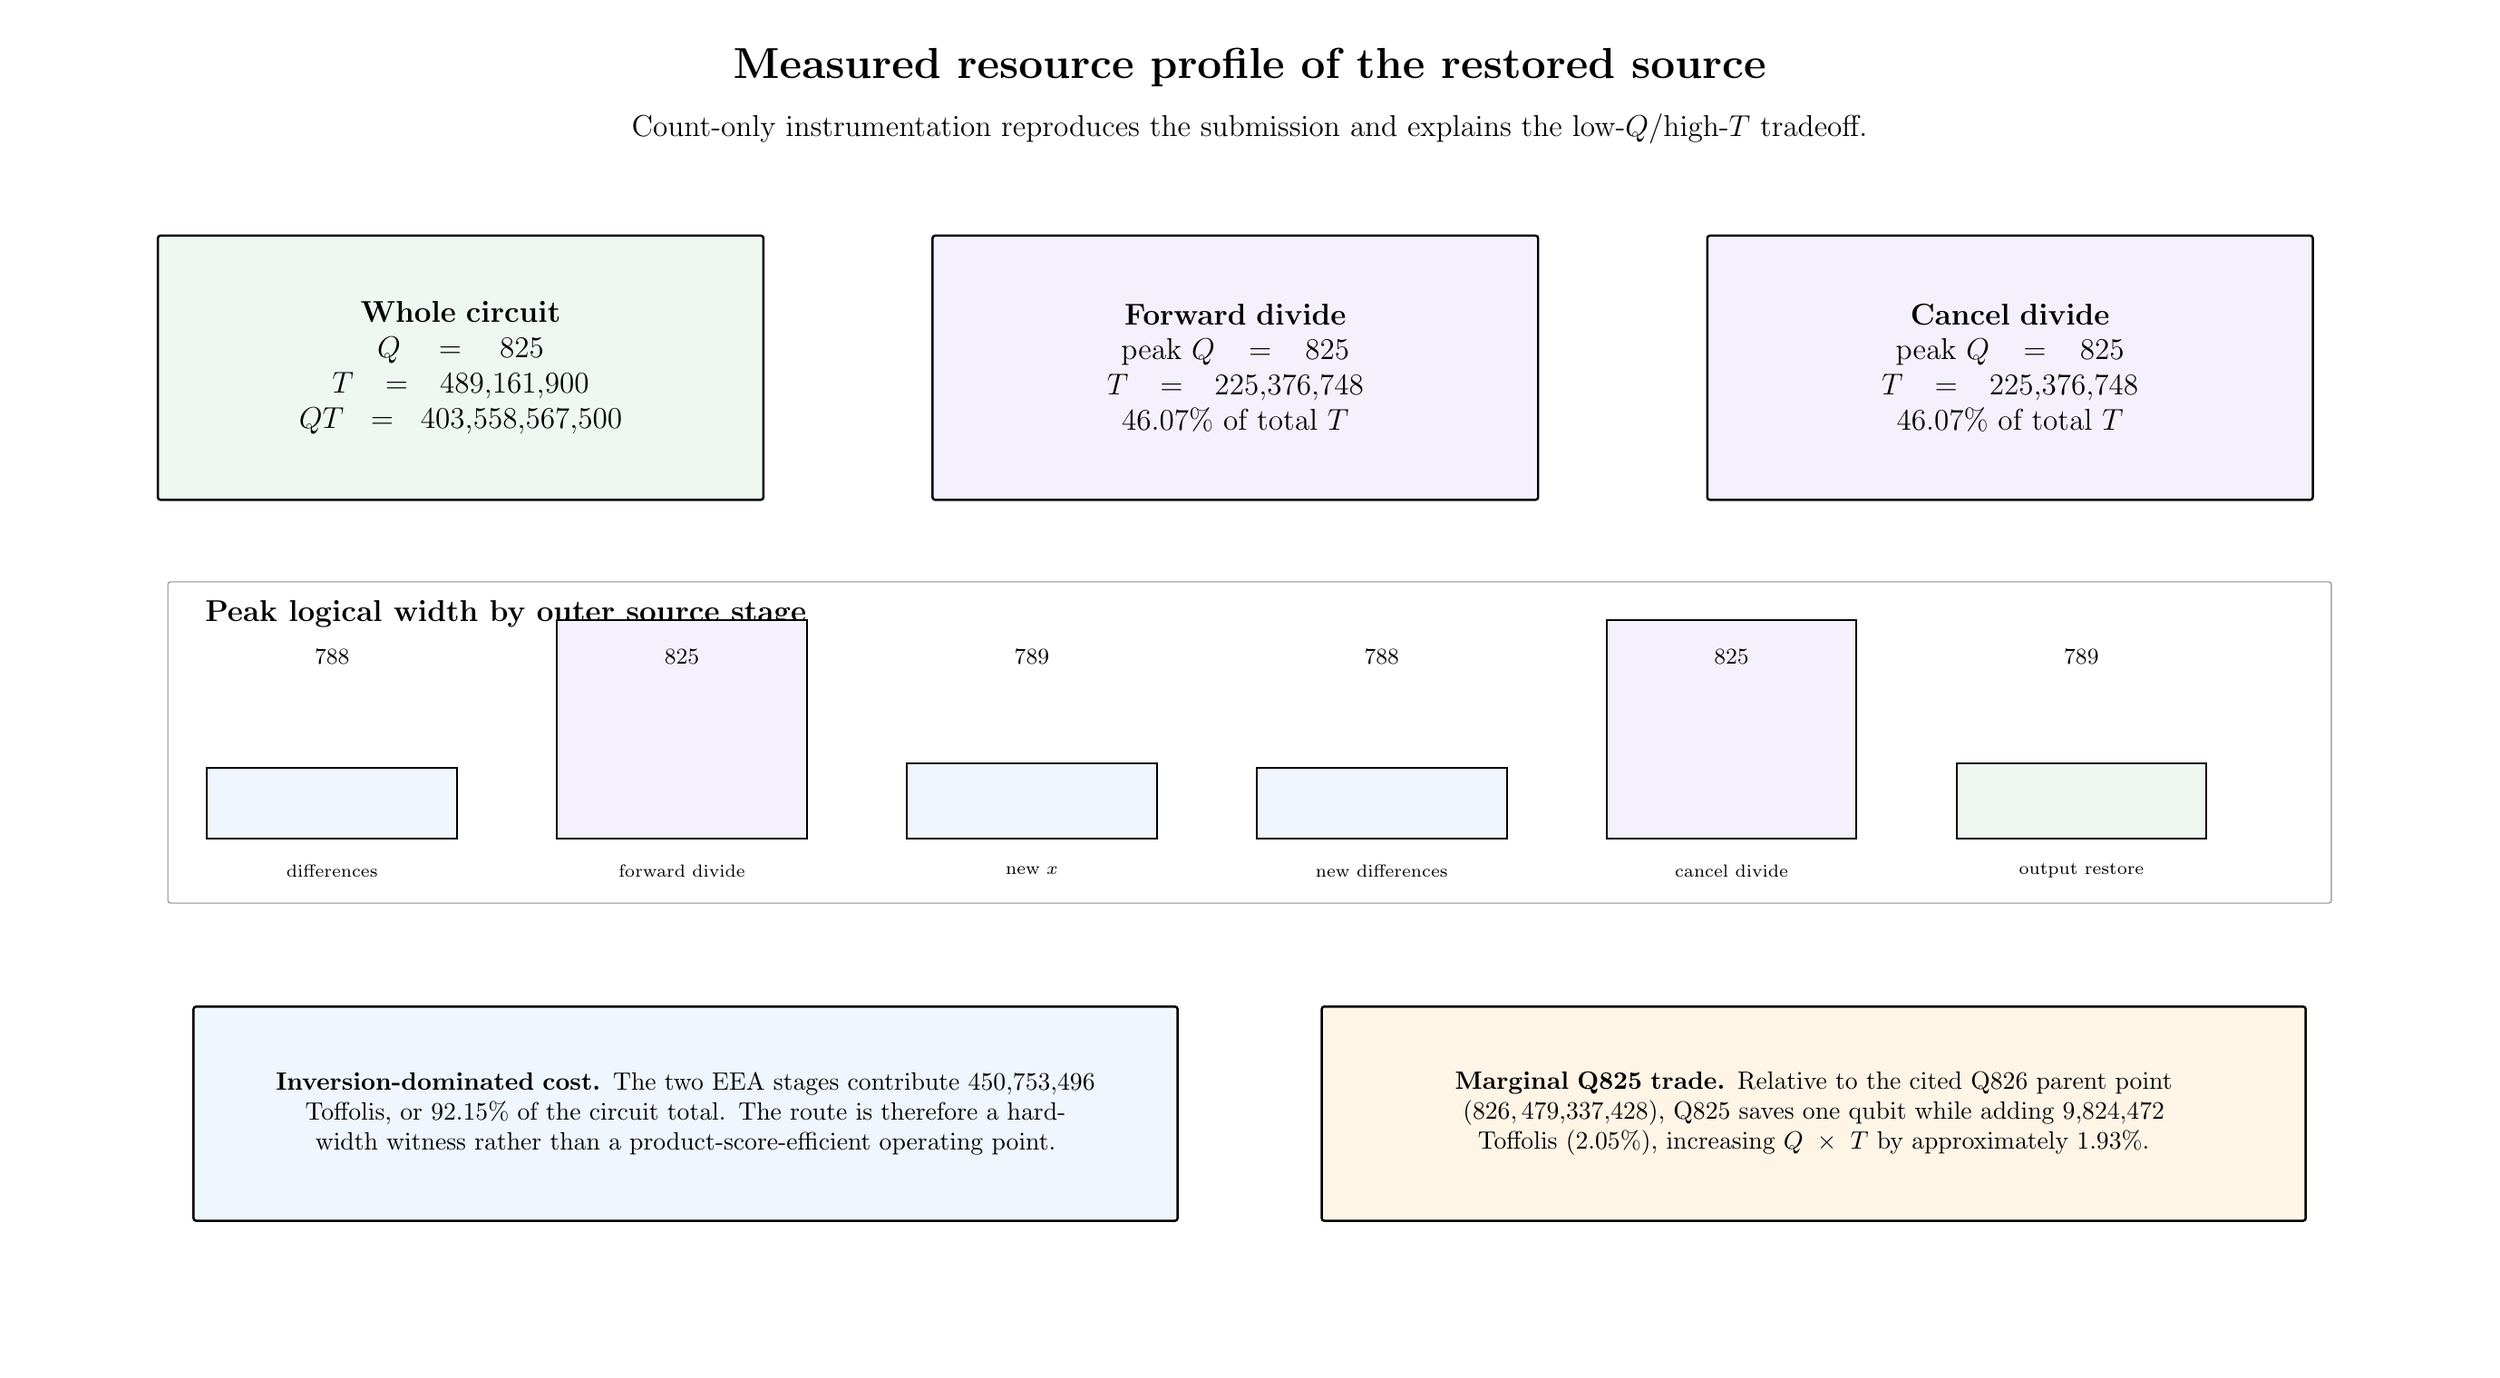
\begin{tikzpicture}[x=1cm,y=1cm]
  \path[use as bounding box] (0,0) rectangle (34.3,18.6);
  \node[font=\LARGE\bfseries] at (17.15,18.0)
    {Measured resource profile of the restored source};
  \node[font=\large] at (17.15,17.15)
    {Count-only instrumentation reproduces the submission and explains the low-$Q$/high-$T$ tradeoff.};

  \node[result,text width=82mm,minimum height=37mm,font=\large] at (6.1,13.8)
    {\textbf{Whole circuit}\\$Q=825$\\$T=489{,}161{,}900$\\$QT=403{,}558{,}567{,}500$};
  \node[inversion,text width=82mm,minimum height=37mm,font=\large] at (16.95,13.8)
    {\textbf{Forward divide}\\peak $Q=825$\\$T=225{,}376{,}748$\\$46.07\%$ of total $T$};
  \node[inversion,text width=82mm,minimum height=37mm,font=\large] at (27.8,13.8)
    {\textbf{Cancel divide}\\peak $Q=825$\\$T=225{,}376{,}748$\\$46.07\%$ of total $T$};

  \draw[black!45,rounded corners=1pt] (2.0,6.3) rectangle (32.3,10.8);
  \node[font=\large\bfseries,anchor=west] at (2.4,10.35) {Peak logical width by outer source stage};
  \fill[gateblue] (2.55,7.2) rectangle (6.05,8.2);
  \fill[invviolet] (7.45,7.2) rectangle (10.95,10.26);
  \fill[gateblue] (12.35,7.2) rectangle (15.85,8.26);
  \fill[gateblue] (17.25,7.2) rectangle (20.75,8.2);
  \fill[invviolet] (22.15,7.2) rectangle (25.65,10.26);
  \fill[outgreen] (27.05,7.2) rectangle (30.55,8.26);
  \foreach \x/\top in {4.3/8.2,9.2/10.26,14.1/8.26,19.0/8.2,23.9/10.26,28.8/8.26}{
    \draw[black,line width=0.7pt] (\x-1.75,7.2) rectangle (\x+1.75,\top);
  }
  \foreach \x/\name/\q in {4.3/{differences}/788,9.2/{forward divide}/825,14.1/{new $x$}/789,19.0/{new differences}/788,23.9/{cancel divide}/825,28.8/{output restore}/789}{
    \node[font=\small\bfseries] at (\x,9.75) {$\q$};
    \node[font=\scriptsize,text width=32mm,align=center] at (\x,6.75) {\name};
  }

  \node[detail,text width=135mm,minimum height=30mm] at (9.25,3.35)
    {\textbf{Inversion-dominated cost.} The two EEA stages contribute $450{,}753{,}496$ Toffolis,
     or $92.15\%$ of the circuit total. The route is therefore a hard-width witness rather than a
     product-score-efficient operating point.};
  \node[classical,text width=135mm,minimum height=30mm] at (25.05,3.35)
    {\textbf{Marginal Q825 trade.} Relative to the cited Q826 parent point
     $(826,479{,}337{,}428)$, Q825 saves one qubit while adding $9{,}824{,}472$ Toffolis
     ($2.05\%$), increasing $Q\times T$ by approximately $1.93\%$.};
\end{tikzpicture}
\newpage

% ============================================================================
% Page 14
% ============================================================================
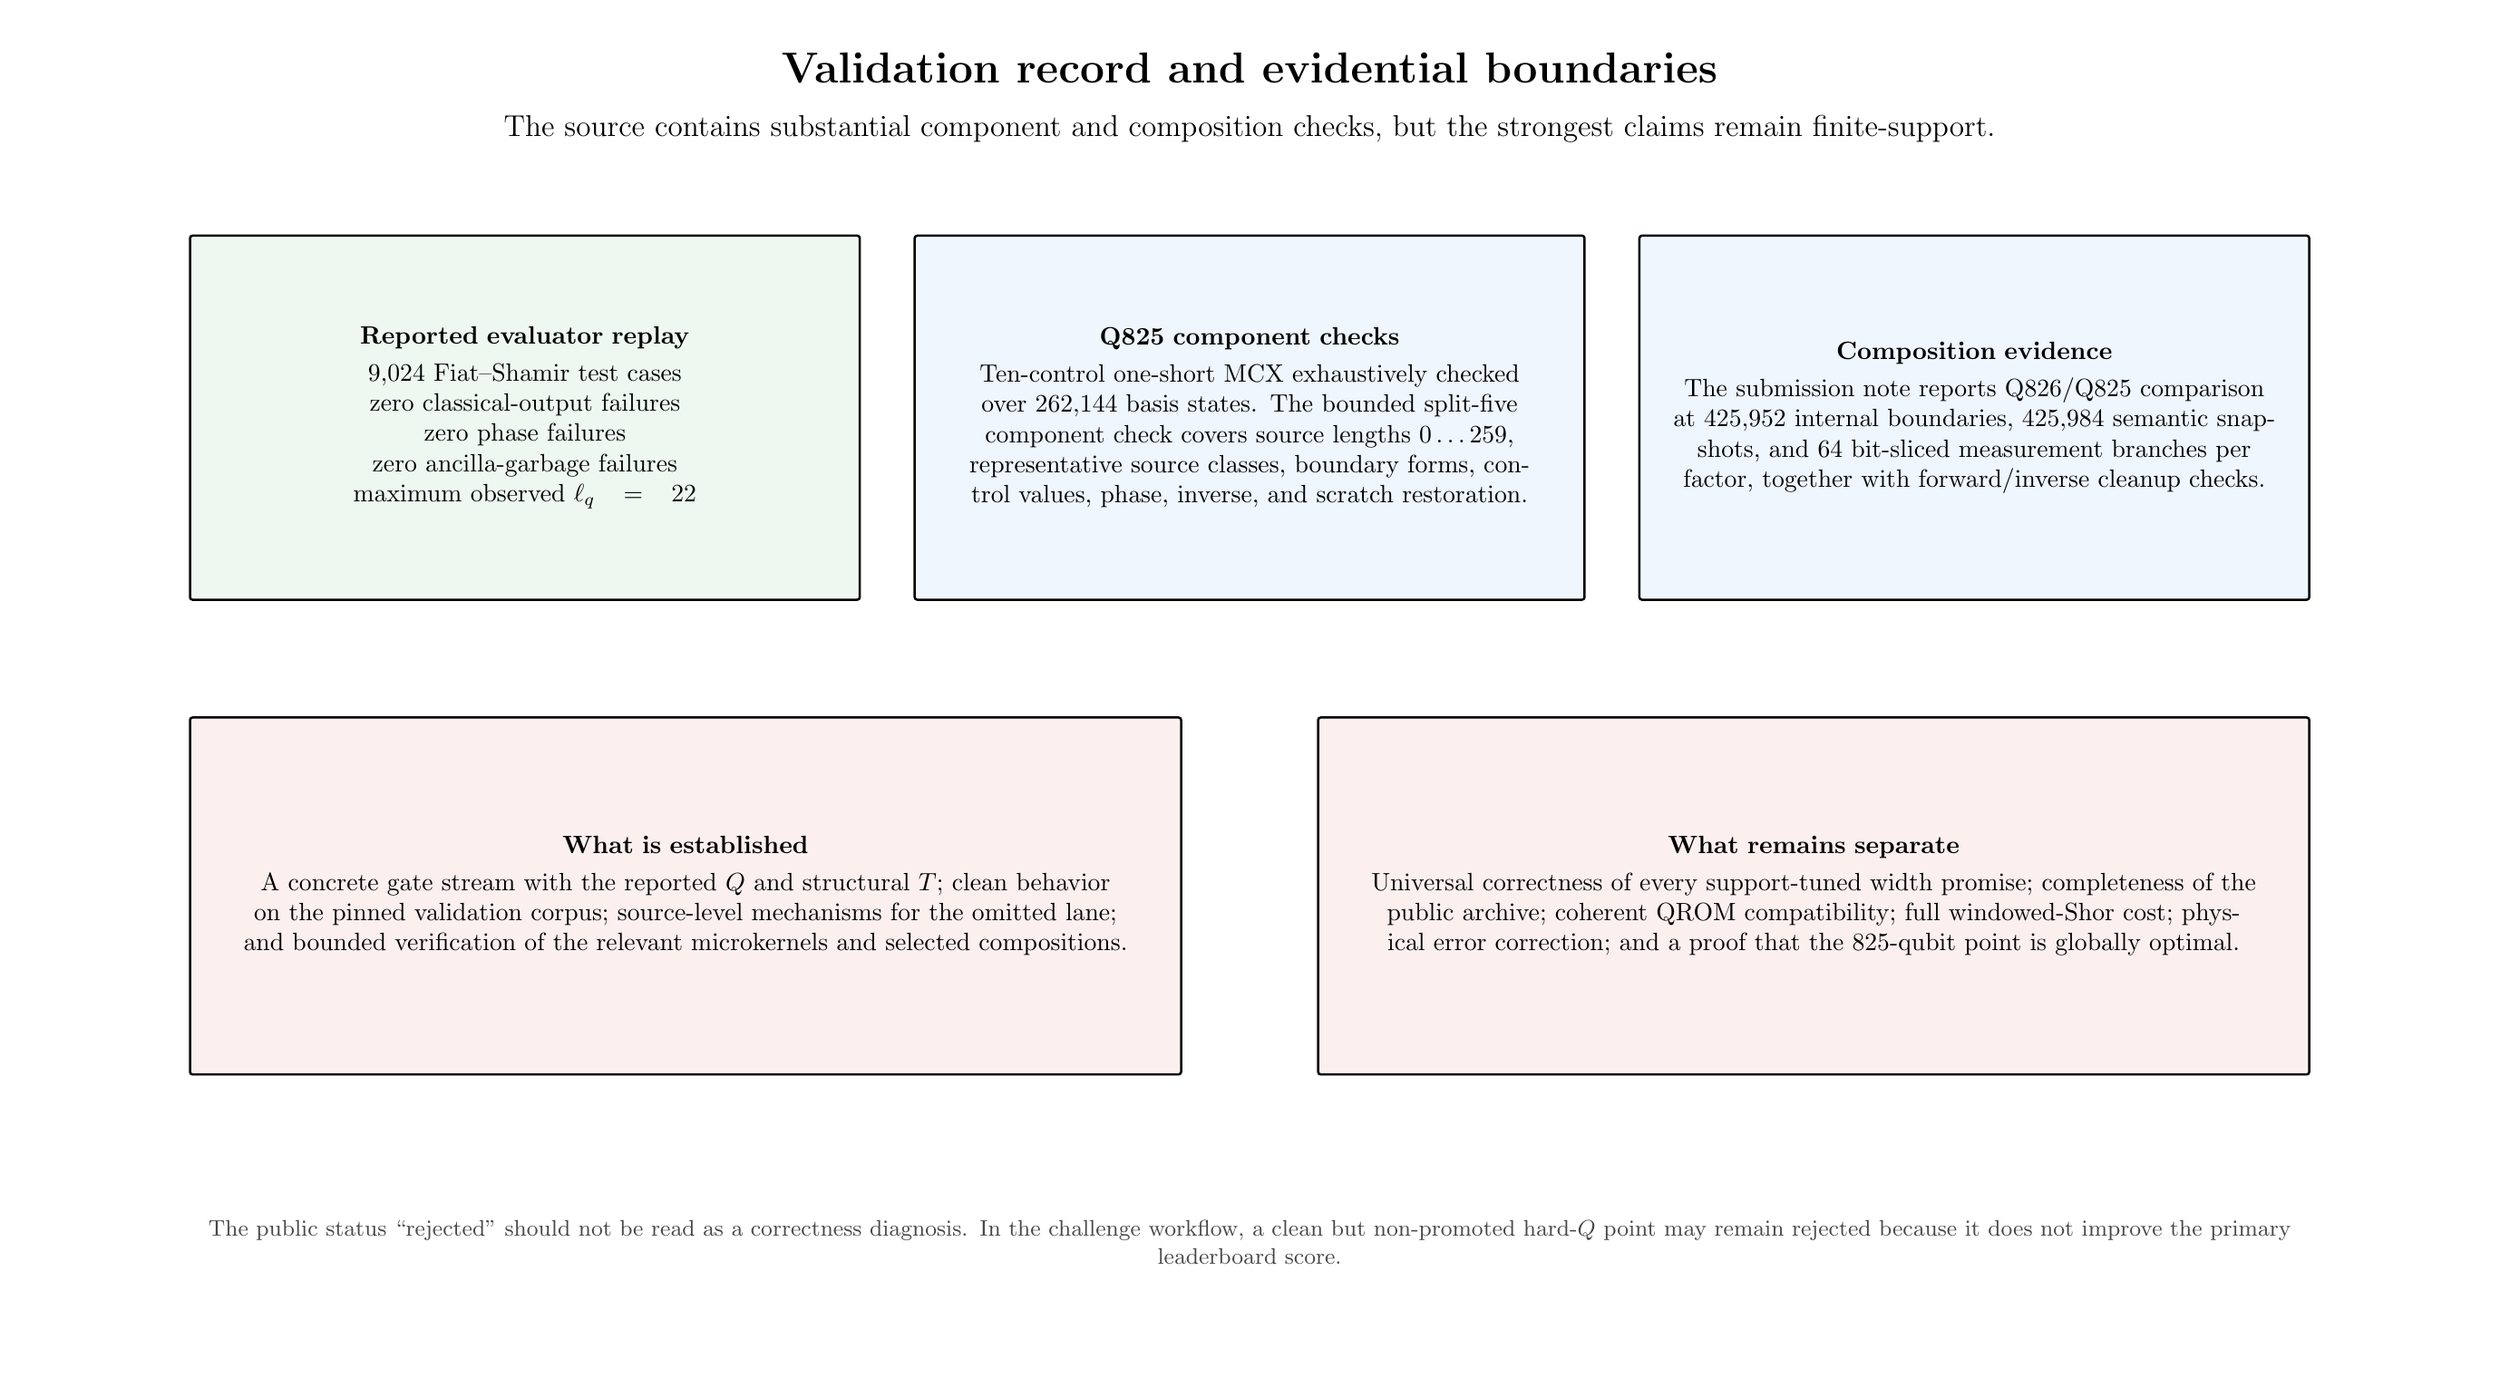
\begin{tikzpicture}[x=1cm,y=1cm]
  \path[use as bounding box] (0,0) rectangle (34.3,18.6);
  \node[font=\LARGE\bfseries] at (17.15,18.0)
    {Validation record and evidential boundaries};
  \node[font=\large] at (17.15,17.15)
    {The source contains substantial component and composition checks, but the strongest claims remain finite-support.};

  \node[result,text width=91mm,minimum height=51mm] at (7.0,13.1)
    {\textbf{Reported evaluator replay}\\[1mm]
     $9{,}024$ Fiat--Shamir test cases\\
     zero classical-output failures\\
     zero phase failures\\
     zero ancilla-garbage failures\\
     maximum observed $\ell_q=22$};
  \node[detail,text width=91mm,minimum height=51mm] at (17.15,13.1)
    {\textbf{Q825 component checks}\\[1mm]
     Ten-control one-short MCX exhaustively checked over $262{,}144$ basis states. The bounded
     split-five component check covers source lengths $0\ldots259$, representative source classes,
     boundary forms, control values, phase, inverse, and scratch restoration.};
  \node[detail,text width=91mm,minimum height=51mm] at (27.3,13.1)
    {\textbf{Composition evidence}\\[1mm]
     The submission note reports Q826/Q825 comparison at $425{,}952$ internal boundaries,
     $425{,}984$ semantic snapshots, and $64$ bit-sliced measurement branches per factor, together
     with forward/inverse cleanup checks.};

  \node[warning,text width=136mm,minimum height=50mm] at (9.25,6.4)
    {\textbf{What is established}\\[1mm]
     A concrete gate stream with the reported $Q$ and structural $T$; clean behavior on the pinned
     validation corpus; source-level mechanisms for the omitted lane; and bounded verification of the
     relevant microkernels and selected compositions.};
  \node[warning,text width=136mm,minimum height=50mm] at (25.05,6.4)
    {\textbf{What remains separate}\\[1mm]
     Universal correctness of every support-tuned width promise; completeness of the public archive;
     coherent QROM compatibility; full windowed-Shor cost; physical error correction; and a proof that
     the 825-qubit point is globally optimal.};

  \node[note,text width=30cm,align=center] at (17.15,1.55)
    {The public status ``rejected'' should not be read as a correctness diagnosis. In the challenge workflow,
     a clean but non-promoted hard-$Q$ point may remain rejected because it does not improve the primary leaderboard score.};
\end{tikzpicture}
\newpage

% ============================================================================
% Page 15
% ============================================================================
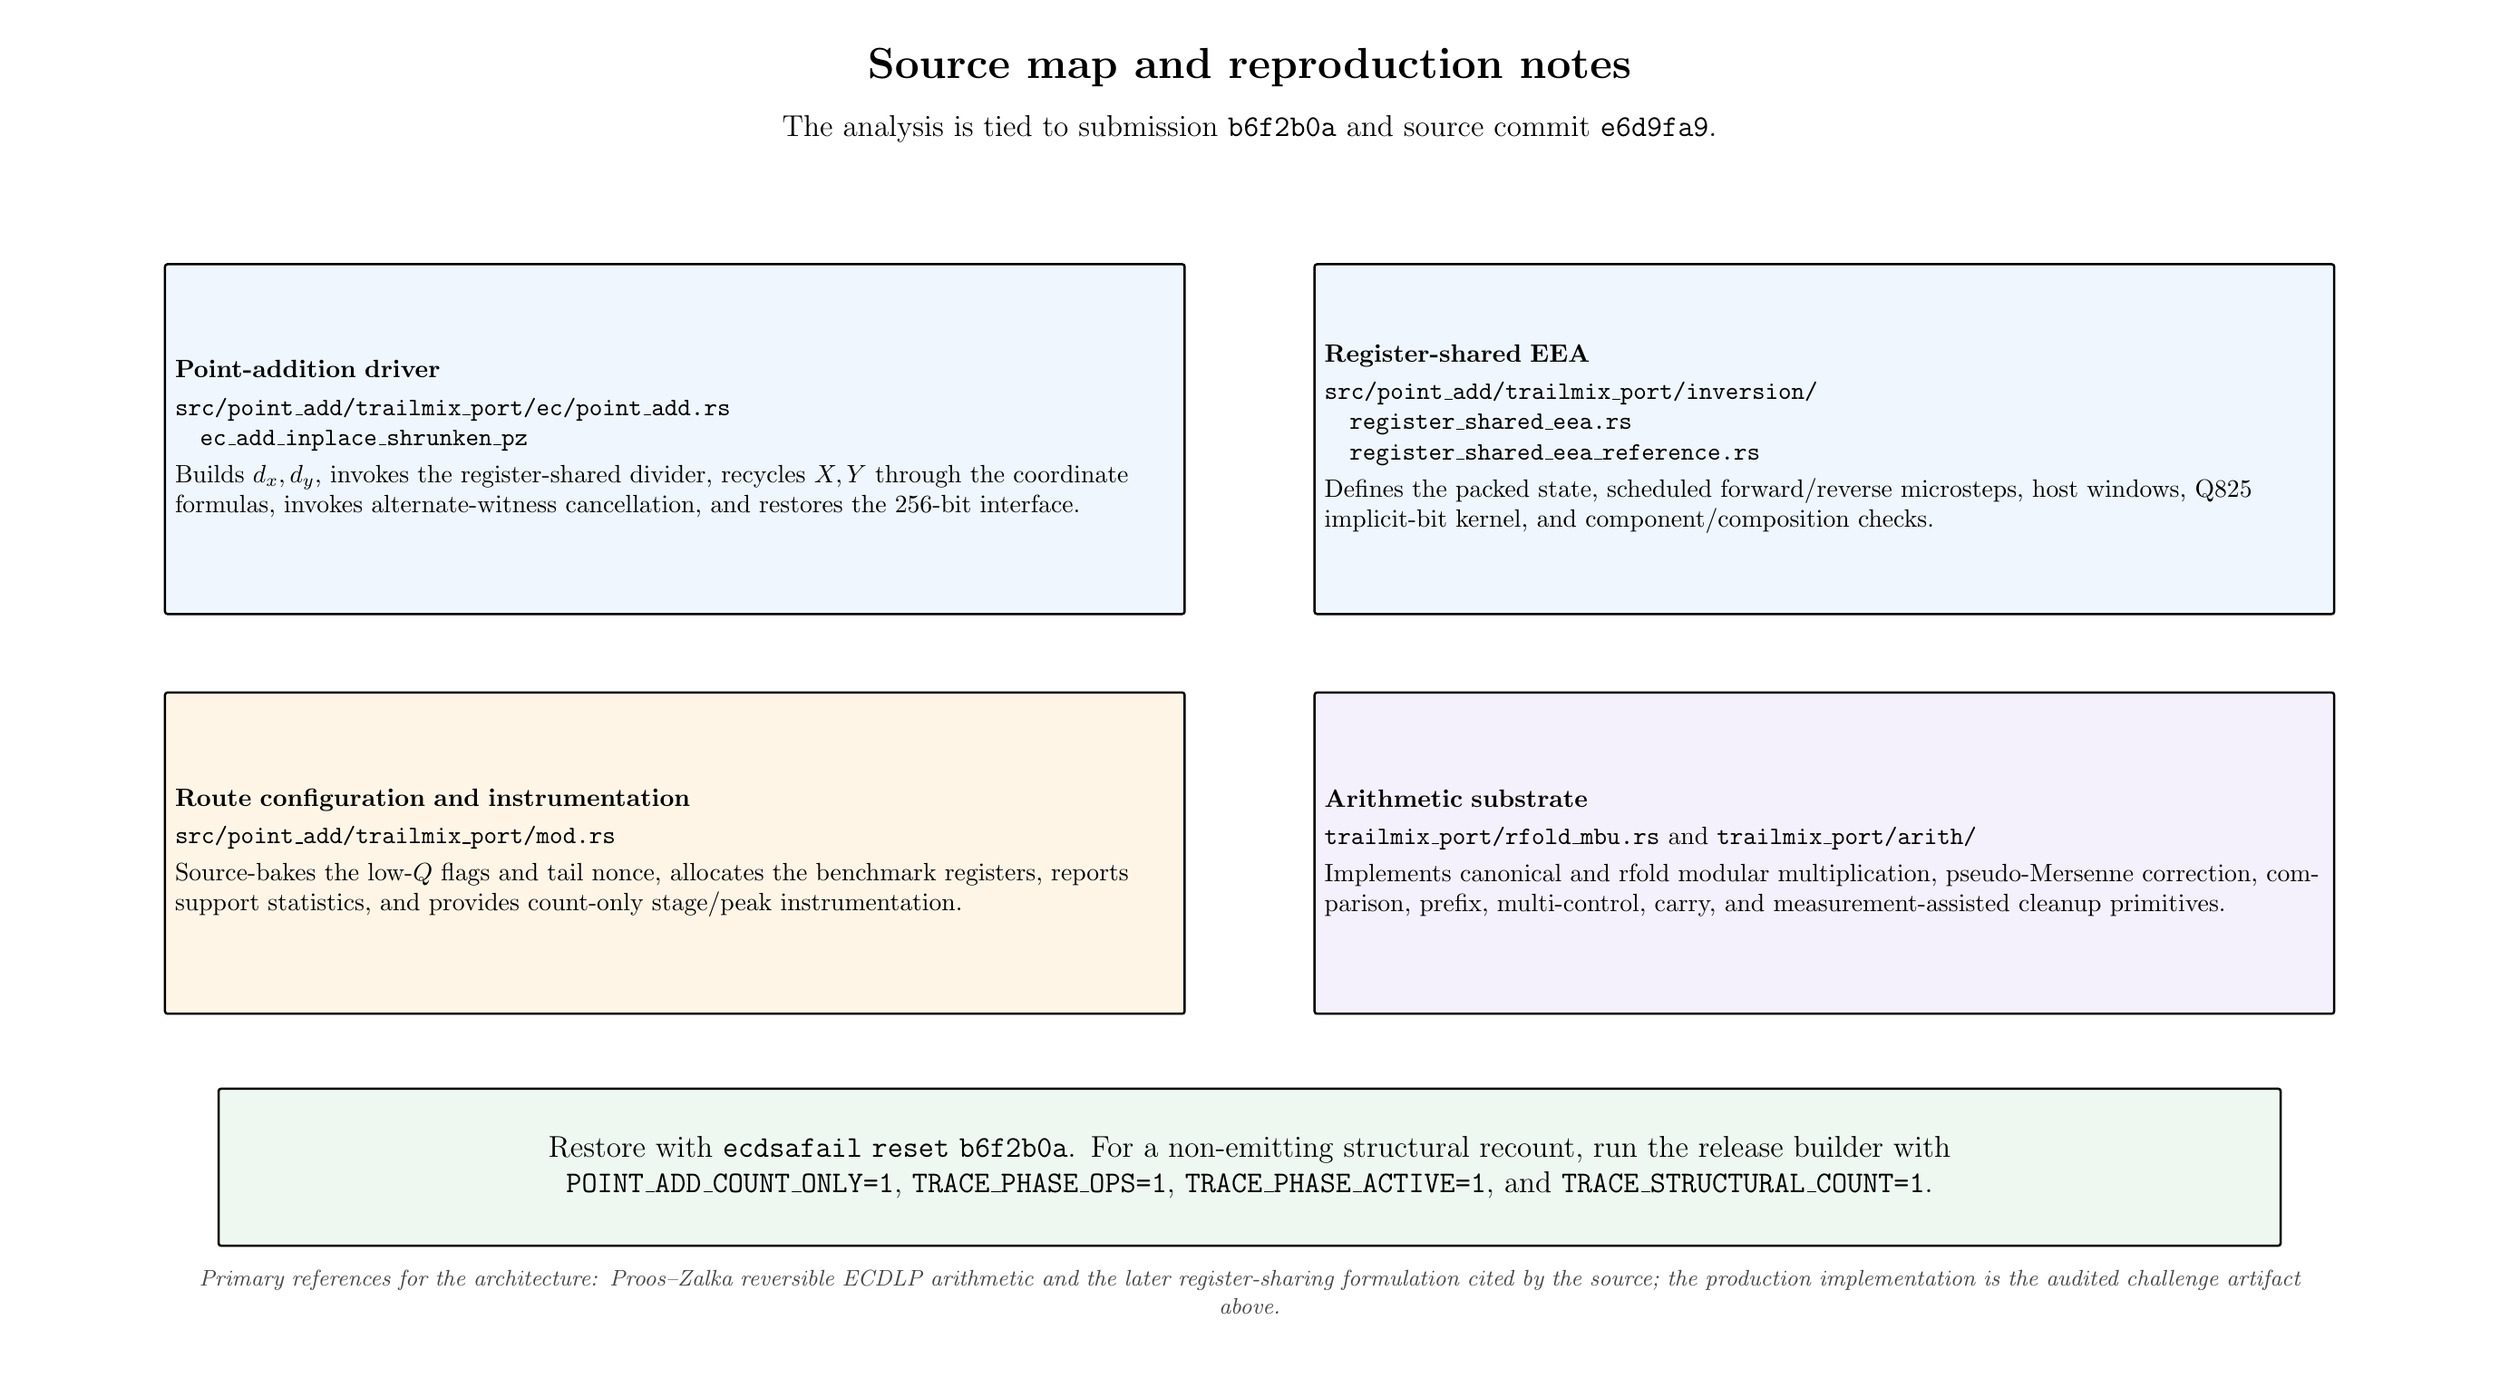
\begin{tikzpicture}[x=1cm,y=1cm]
  \path[use as bounding box] (0,0) rectangle (34.3,18.6);
  \node[font=\LARGE\bfseries] at (17.15,18.0)
    {Source map and reproduction notes};
  \node[font=\large] at (17.15,17.15)
    {The analysis is tied to submission \texttt{b6f2b0a} and source commit \texttt{e6d9fa9}.};

  \node[detail,text width=140mm,minimum height=49mm,align=left] at (9.1,12.8)
    {\textbf{Point-addition driver}\\[1mm]
     \texttt{src/point\_add/trailmix\_port/ec/point\_add.rs}\\
     \quad\texttt{ec\_add\_inplace\_shrunken\_pz}\\[1mm]
     Builds $d_x,d_y$, invokes the register-shared divider, recycles $X,Y$ through the
     coordinate formulas, invokes alternate-witness cancellation, and restores the $256$-bit interface.};
  \node[detail,text width=140mm,minimum height=49mm,align=left] at (25.2,12.8)
    {\textbf{Register-shared EEA}\\[1mm]
     \texttt{src/point\_add/trailmix\_port/inversion/}\\
     \quad\texttt{register\_shared\_eea.rs}\\
     \quad\texttt{register\_shared\_eea\_reference.rs}\\[1mm]
     Defines the packed state, scheduled forward/reverse microsteps, host windows,
     Q825 implicit-bit kernel, and component/composition checks.};

  \node[classical,text width=140mm,minimum height=45mm,align=left] at (9.1,7.0)
    {\textbf{Route configuration and instrumentation}\\[1mm]
     \texttt{src/point\_add/trailmix\_port/mod.rs}\\[1mm]
     Source-bakes the low-$Q$ flags and tail nonce, allocates the benchmark registers,
     reports support statistics, and provides count-only stage/peak instrumentation.};
  \node[inversion,text width=140mm,minimum height=45mm,align=left] at (25.2,7.0)
    {\textbf{Arithmetic substrate}\\[1mm]
     \texttt{trailmix\_port/rfold\_mbu.rs} and \texttt{trailmix\_port/arith/}\\[1mm]
     Implements canonical and rfold modular multiplication, pseudo-Mersenne correction,
     comparison, prefix, multi-control, carry, and measurement-assisted cleanup primitives.};

  \node[result,text width=286mm,minimum height=22mm,font=\large] at (17.15,2.6)
    {Restore with \texttt{ecdsafail reset b6f2b0a}. For a non-emitting structural recount, run the
     release builder with \texttt{POINT\_ADD\_COUNT\_ONLY=1}, \texttt{TRACE\_PHASE\_OPS=1},
     \texttt{TRACE\_PHASE\_ACTIVE=1}, and \texttt{TRACE\_STRUCTURAL\_COUNT=1}.};

  \node[note,text width=30cm,align=center,font=\small\itshape] at (17.15,0.85)
    {Primary references for the architecture: Proos--Zalka reversible ECDLP arithmetic and the later
     register-sharing formulation cited by the source; the production implementation is the audited challenge artifact above.};
\end{tikzpicture}

\end{document}
